%%%%%%%%%%%%%%%%%%%%%%%%%%%%%%%%%%%%%%%%%
%  Mascaret Documentation
%  Theory guide
%
%%%%%%%%%%%%%%%%%%%%%%%%%%%%%%%%%%%%%%%%%

%----------------------------------------------------------------------------------------
%	PACKAGES AND OTHER DOCUMENT CONFIGURATIONS
%----------------------------------------------------------------------------------------
\documentclass[Mascaret]{../../data/TelemacDoc} % Default font size and left-justified equations

%%---------------------------------------------------------------------------
%%Equations
%%---------------------------------------------------------------------------
\renewcommand{\Grad}{\vec \nabla}
\renewcommand{\Div}{\nabla \cdot}
\renewcommand{\Lap}{\nabla^2}%{\text{lap}\hspace{0.1em}}
\newcommand{\BDiv}{\vec{\nabla} \cdot}
\newcommand{\BLap}{\vec{\nabla}^2}
\newcommand{\DivD}{\nabla_{2D} \cdot}
\newcommand{\Divast}{\nabla^* \cdot}

%%---------------------------------------------------------------------------
%% Tableaux
%%---------------------------------------------------------------------------
%\usepackage{booktabs,multirow}
%\usepackage{lscape}
%\usepackage{longtable}
%\newcommand{\minitab}[2][1]{\begin{tabular}{#1}#2\end{tabular}}
%%\usepackage{array}
%%\newcolumntype{L}[1]{>{\raggedright\let\newline\\\arraybackslash\hspace{0pt}}m{#1}}
%%\newcolumntype{C}[1]{>{\centering\let\newline\\\arraybackslash\hspace{0pt}}m{#1}}
%%\newcolumntype{R}[1]{>{\raggedleft\let\newline\\\arraybackslash\hspace{0pt}}m{#1}}

%%---------------------------------------------------------------------------
%% Nomenclature
%%---------------------------------------------------------------------------
\usepackage{ifthen}
\usepackage{nomencl}
%
\makenomenclature
\renewcommand{\nompreamble}{\markboth{%
                            \MakeUppercase\nomname}{\MakeUppercase\nomname}%
                           }

\renewcommand{\nomgroup}[1]{
\ifthenelse{\equal{#1}{C}}{\item[\textbf{In the continuous domain}]}{
\ifthenelse{\equal{#1}{D}}{\item[\textbf{In the discrete domain}]}{
{}
}% matches discrete domain
}% matches continuous domain
}

\begin{document}

\let\cleardoublepage\clearpage
%----------------------------------------------------------------------------------------
%	TITLE PAGE
%----------------------------------------------------------------------------------------
\title{\mascaret}
\subtitle{Theory guide}
\version{\telmaversion}
\date{\today}
\maketitle
\clearpage

%----------------------------------------------------------------------------------------
%	AUTHORS PAGE
%----------------------------------------------------------------------------------------

\newpage

\thispagestyle{empty}

\chapter*{Authors and contributions}
This document was first created in French by Nicole GOUTAL (EDF) and Fabrice ZAOUI (EDF)

The translation was done by HR Wallingford

This version which comply with the official template of \telemacsystem{} was created by Christophe Coulet (ARTELIA).

\newpage

\chapter*{Work under construction}\label{workunderconstruction}
We would like to warn the reader that this document is still under construction
and could be improved in many ways. Any remarks, suggestions, corrections, etc.
are welcome and can be submitted to the \telemacsystem development team through
the forum in the Documentation category:
\url{http://www.opentelemac.org/index.php/kunena/10-documentation}.

\newpage

\chapter*{Abstract}\label{Abstract}
Developed for more than 20 years by Electricité De France (EDF) and the Centre d'Etudes et d'Expertise sur les Risques, l'Environnement, la Mobilité et l'Aménagement (CEREMA), \mascaret{} is a hydraulic modelling software dedicated to one-dimensional free-surface flow, based on the Saint-Venant equations.
\mascaret{} includes three computational engines, all of which can be coupled to the \casier{} module in order to represent quasi-2D floodplain storage. The three engines can respectively represent the following flows:

\begin{itemize}
 \item Subcritical and Transcritical steady;
 \item Subcritical unsteady;
 \item Transcritical unsteady.
\end{itemize}

The \casier{} module represents water storage and movement on the floodplain with storage areas that can be connected to the river channel and connected to each other. Various relations can be used to represent these connections: weir, channel, siphon, orifice.
\mascaret{} is suited for the following types of project:

\begin{itemize}
 \item River and floodplain inundation modelling;
 \item Floodwave propagation after a hydraulic structure failure;
 \item Discharge regulation in rivers and canals;
 \item Wave propagation in canals (intumescence, lockage water, priming).
\end{itemize}

This report is the theoretical note for the software \mascaret{} and its algorithms. The principles of the mathematical modelling of one-dimensional free-surface flow used by the computational engines of \mascaret{} are presented here, as well as the numerical methods used to solve the equations for subcritical and transcritical flow. The principles of the storage areas module \casier{} and the methods for coupling it with \mascaret{} are also described, as well as the principles of the automatic calibration module.



%----------------------------------------------------------------------------------------
%	COPYRIGHT PAGE
%----------------------------------------------------------------------------------------

\newpage

\thispagestyle{empty}

\TelemacCopyright{}


%----------------------------------------------------------------------------------------
%	TABLE OF CONTENTS
%----------------------------------------------------------------------------------------


\pagestyle{empty} % No headers

\tableofcontents% Print the table of contents itself

\pagestyle{fancy} % Print headers again

%----------------------------------------------------------------------------------------
%	The whole thing
%----------------------------------------------------------------------------------------
%%===========================================================================
%\section{Reminders and definition of variables}
%%===========================================================================
%
%Bold variables will represent vectors and tensors, and plain font will represent scalars; i.e.:
%
%\begin{align}
%\vec{A} = \left[\begin{array}{c}
%		A_x
%		\\
%		A_y
%		\\
%		A_z
%		\end{array}\right]
%\end{align}
%
%Furthermore, the following operators are defined:
%
%\begin{subequations}
%\begin{align}
%\Grad\{A\}		= & \vec{\nabla} A
%\\
%\Grad\{\vec{A}\}		= & \vec{\nabla} \vec{A}^T
%\\
%\Div\{\vec{A}\}	= & \vec{\nabla} \cdot \vec{A}
%\\
%\Lap\{B,A\} =	& \vec{\nabla} \cdot \left( B\vec{\nabla} A\right)
%\notag\\
%			=	& \Div\{B\Grad\{A\}\}
%\\
%\BLap\{B,\vec{A}\} =	& \vec{\nabla} \cdot \left( B\vec{\nabla} \vec{A}^T\right)
%\notag\\
%						=	& \Div\{B\Grad\{\vec{A}\}\}
%\end{align}
%\end{subequations}
%
%Where $\vec{\nabla}$ is the nabla operator defined as:
%
%\begin{align}
%\vec{\nabla} = \left[\begin{array}{c}
%		\dfrac{\partial}{\partial x}
%		\\[1em]
%		\dfrac{\partial}{\partial y}
%		\\[1em]
%		\dfrac{\partial}{\partial z}
%		\end{array}\right]
%\end{align}
%
%In addition $\vec{A}^T$ is the transpose of vector $\vec{A}$.

%===========================================================================
% Nomenclature
%===========================================================================

\printnomenclature

%----------------------------------------------------------------------------------------
%	CHAPTER 1: Introduction and general hypothesis
%----------------------------------------------------------------------------------------

%-------------------------------------------------------------------------------
\chapter{Introduction and general hypothesis}
\label{Chapter1}
%-------------------------------------------------------------------------------

%-------------------------------------------------------------------------------
\section{Introduction}
%-------------------------------------------------------------------------------

This report sets out the mathematical modelling of one-dimensional subcritical
and supercritical flows on which the three different hydraulic engines of the
code system \mascaret{} are based, as well as the methods of solving
equations resulting from these models.
We present below the structure of the \mascaret{} system. This report
only covers the \textit{hydraulic} part of the system.

\begin{figure}[h]
 \begin{center}
  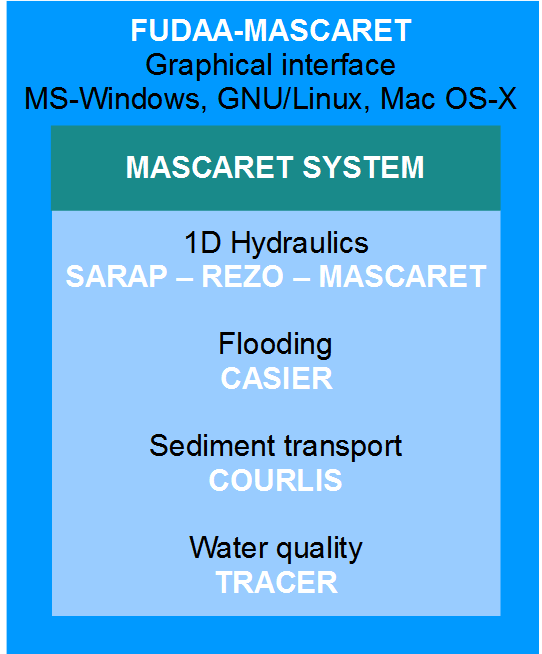
\includegraphics[width=0.5\textwidth]{Figures/MASCARET_system.png}
  \caption{The \mascaret{} software}
 \end{center}
\end{figure}

The numerical methods used vary depending on whether the flows are steady or
unsteady, subcritical or supercritical and also depending on the type of
hydraulic network : branched network (subcritical steady flow engine) or meshed
network (subcritical unsteady flow engine). It is recalled that any branch
arrangement are allowed in a meshed network, whilst in a branched network there
is only one single path connecting two points of the network.

%-------------------------------------------------------------------------------
\section{General hypothesis}
%-------------------------------------------------------------------------------

The principal hypotheses justifying the modelling approach (1-D) used in the 3
hydraulic engines are stated below:

\begin{itemize}
 \item each reach has a prefered axis of flow, the velocity vectors are always
   considered parallel to this axis ;
 \item the flow has a small curvature in the horizontal plane ; the vertical
   accelerations are negligible, and the distribution of pressures is
   quasi-hydrostatic ;
 \item the average slope of the flow is small (the cosine of the angle between
   the horizontal and the bottom is close to 1) ;
 \item the viscosity shear stress on the bottom and the banks are taken into
   account using empirical friction laws (Strickler's relation).
\end{itemize}

Therefore, in each plane perpendicular to its axis, the flow is entirely determined by the values of the average velocity (or of the total flow), and of the elevation of the free surface.

A few other hypotheses are also considered in order to simplify the data entry process and consider only the most usual cases :

\begin{itemize}
 \item the influence of the wind is neglected;
 \item when a confluent is not modelled using a specific reach, it is assumed perpendicular to the main axis of flow: it is represented by a lateral flow input that does not add any momentum.
\end{itemize}

Other codes developed at EDF can be used when the hypotheses associated with \mascaret{} are too limiting, and complement the engines provided by \mascaret{}.

\begin{itemize}
 \item Two-dimensional flows can be treated with the \telemac{2D} system\cite{hervouet07};
 \item The geometry of the reaches is not evolving during the simulations. The \courlis{} code, which uses the hydraulic engine of \mascaret{}, is dedicated to the treatment of solid transport and its consequences ;
 \item Extended inundation plains, where the flows is not one-dimensional, can be modelled with a system of inter-connected storage cells. The \casier{} code can be linked to the unsteady subcritical flow engine to widens the field of application of the \mascaret{} system. It represents a network of reaches and associated storage cells (equivalent to quasi-2d modelling)
\end{itemize}

%-------------------------------------------------------------------------------
\section{Definitions and notations}
%-------------------------------------------------------------------------------

%...............................................................................
\subsection{Definitions} \label{secDef}
%...............................................................................

In the introduction we have outlined the basic characteristics of the modelling.  We consider subcritical and supercritical flows in networks of reaches, each reach having a principal axis of flow. The calculated values are always relative to a section of flow perpendicular to this axis, each section is identified by its abscissa along this axis.

The flow sections are considered to be the union of the three sub-sections:

\begin{itemize}
 \item \underline{The low flow channel}, normal channel outside of flood periods. This channel can include islands but, if so, the elevation of the free surface is supposed to be identical on each side of the island. If this is not the case, one should resort to use a meshed network model ;
 \item \underline{The high flow channel}, additional sections of flow active in times of flood, when the water level rises above the crest of the right or left bank. These sections are represented on each side of the channel, the elevation of the two banks being generally distinct ;
 \item \underline{The storage zones}, treated like reservoirs, fill up as the flood rise and empty as water levels decrease. They act as water storage but, unlike the high flow channel, they do not convey any flow (the velocities in the direction of the axis of flow are supposed nil).
\end{itemize}

If the low flow channel is generally easy to identify, the limit between the high flow channel and storage zones is however much less well defined and can vary depending on the importance of the flood.

When the storage zones are likely to generate transverse flows in the floodplain, the present modeling approach becomes insufficient ; it is therefore necessary to couple \mascaret{} with a storage cell system.

It can be necessary to use a two-dimensional model instead of or in complement to the one-dimensional model, when the one-dimensional approach reaches its limits.

The estimation of the energy dissipated by friction is a fundamental element of the modelling. This is usually done with the Strickler roughness coefficient (see the following paragraph), it should be estimated separately in the low flow or high flow channel. The role of the calibration is to estimate the friction coefficients as well as possible by using the known natural level of the water. This calibration is often done by trial and errors. However, an optimisation algorithm has been specially developed for the steady flow engine, and this allows an automatic calibration of the friction coefficients.

Figure \ref{fig:SchemProf} and its notations summarise the key elements of the modelling approach in a flow section.

\begin{figure}[H]
 \begin{center}
  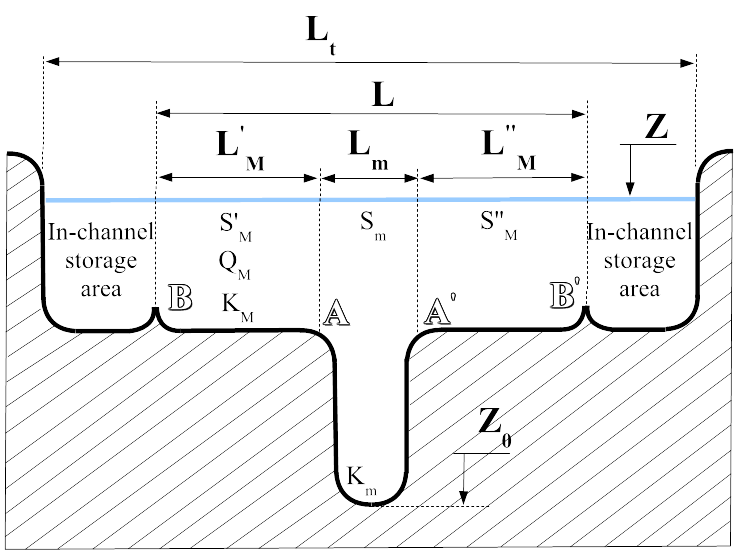
\includegraphics[width=0.8\textwidth]{Figures/Schema_profil.png}
  \caption{Representation of a profile - Notations}
  \label{fig:SchemProf}
 \end{center}
\end{figure}

\begin{CommentBlock}{Comment :}
it is important to distinguish between the ``data'' sections (or profiles) where the geometry is calculated directly from topographic information (survey, digital terrain model), and the ``computation'' sections (chosen by the user) where the values will be obtained by interpolation between ``data'' profiles.
\textit{In the computational sections, the flow variables are interpolated between data sections, not the bathymetry/geometry}
\end{CommentBlock}

%...............................................................................
\subsection{Notations} \label{secNot}
%...............................................................................

Unless otherwise stated, the following variables are used throughout the document (see figure \ref{fig:SchemProf}) :

\begin{itemize}
 \item $t$ the time ($s$);
 \item $x$ the abscissa along the principal axis of flow in the river ($m$); \newline

 \item $Q_m$ the discharge in the low flow channel ($m^3.s^{-1}$);
 \item $Q_M$ the discharge in the high flow channel, left and right bank ($m^3.s^{-1}$);
 \item $Q$ the total discharge in the active channel ($m^3.s^{-1}$) : $Q = Q_m + Q_M$;
 \item $q_l$ the lateral inflow contribution per meter length ($m^2.s^{-1}$); \newline

 \item $L_m$ the surface width of the low flow channel ($m$);
 \item $L_M$ the surface width of the high flow channel ($m$) : $L_M = L^{'}_{M} + L^{''}_M$;
 \item $L$ the surface width of the active channel ($m$) : $L = L_m + L_M$;
 \item $L_s$ the width of the storage zones ($m$);
 \item $L_t$ the surface width of the total channel with storage ($m$); \newline

 \item $S_m$ the area of the low flow channel or wetted cross section ($m^2$);
 \item $S_M$ the area of the high flow channel ($m^2$) : $S_M = S^{'}_{M} + S^{''}_M$;
 \item $S$ the area of the active bed ($m^2$) : $S = S_m + S_M$;
 \item $S_s$ the area of the active channel ($m^2$);
 \item $S_t$ the area of the total channel with storage ($m^2$); \newline

 \item $K_m$ the Strickler coefficient of the low flow channel;
 \item $K_M$ the Strickler coefficient of the high flow channel; \newline

 \item $P_m$ the wetted perimeter of the low flow channel ($m$) : $P_m = AA^{'}$;
 \item $P_M$ the wetted perimeter of the high flow channel ($m$) : $P_M = A^{'}B^{'}+AB$;
 \item $P$ the wetted perimeter of the active channel ($m$) : $P = P_m + P_M$; \newline

 \item $R_m$ the hydraulic radius of the low flow channel ($m$) : $R_m = S_m / P_m$;
 \item $R_M$ the hydraulic radius of the high flow channel ($m$) : $R_M = S_M / P_M$;
 \item $R$ the hydraulic radius of the active channel ($m$) : $R = S / P$; \newline

 \item $V_m$ the velocity of water in the low flow channel ($m.s^{-1}$) : $V_m = Q_m / S_m$;
 \item $V_M$ the velocity of water in the high flow channel ($m.s^{-1}$) : $V_M = Q_M / S_M$;
 \item $V$ the mean velocity of the flow ($m.s^{-1}$) : $V = Q / S$;
\end{itemize}


%----------------------------------------------------------------------------------------
%	CHAPTER 2: The F.D. Engines
%----------------------------------------------------------------------------------------
%-------------------------------------------------------------------------------
\chapter{The steady \SARAP{} and unsteady \REZO{} Finite Differences engines}
\label{Chapter2}
%-------------------------------------------------------------------------------

%-------------------------------------------------------------------------------
\section{The modelling principles}
%-------------------------------------------------------------------------------

%...............................................................................
\subsection{Definitions and notations}
%...............................................................................

The hypotheses and notations are presented in sections \ref{secDef} and \ref{secNot} respectively.

%...............................................................................
\subsection{Basic modelling of a reach with low flow}
%...............................................................................

We use the well-established Saint-Venant equations :

\begin{itemize}
 \item the continuity equation :
   \begin{equation}
     \label{masse}
     \frac{\partial Q}{\partial x} + \frac{\partial S}{\partial t}= q_l
   \end{equation}
   with :
   \begin{itemize}
     \item $Q(x,t)$ the flow ($m^3.s^{-1}$);
     \item $Z(x,t)$ the elevation of the free surface ($m$).
   \end{itemize}
 \item and the momentum equation :
   \begin{equation}
     \label{qmv}
     \frac{\partial Q}{\partial t} + \frac{\partial}{\partial x}\left( {\beta \frac{Q^2}{S}} \right) + g S \left( \frac{\partial Z}{\partial x} + J \right) = \gamma_l
   \end{equation}
   with $g$ the acceleration of gravity ($m.s^{-2}$).

\end{itemize}

The continuity equation relates to the conservation of the flow, the momentum equation corresponds to the fundamental equation of dynamics: the first member represents the accelleration of a \textit{volume of water}; the second member represents the sum of the forces applied to it.

When there is no lateral inflow : $q_l = \gamma_l = 0$. In the case of a lateral inflow, the version $7.1.4$ introduces two possible choices :

\begin{itemize}
 \item the inflow is considered perpendicular to the flow and does not bring any momentum : $\gamma_l = 0$
 \item the inflow modifies the momentum equation : $\gamma_l = \frac{Q}{S}q_l$
\end{itemize}

The term $gSJ$ relates to the effect of friction : $J$ is a dimensionless number, representing the average rate of the energy dissipation. It depends on the flow, the hydraulic characteristics of the river and of course, on the roughness coefficient. It is calculated with the Strickler relation:

   \begin{equation}
     J = \frac{Q^2}{K_{m}^{2}S^{2}R^{4/3}}
   \end{equation}
where
   \begin{equation}
     J = \frac{Q^2}{D^2}
   \end{equation}

with :
\begin{itemize}
 \item $K_m$ the Strickler's roughness coefficient;
 \item $R$ the hydraulic radius;
 \item $D$ the conveyance.
\end{itemize}

The dimensionless coefficient $\beta$ results from the variations of the actual flow velocity in a section. These variations would otherwise be ignored as only the average velocity is considered in the one-dimensional equations. The definition of $\beta$ is :

   \begin{equation}
     \beta = \frac{S}{Q^2} \int V^2 \,dS
   \end{equation}

Taking into account the hypotheses described previously (see section \ref{secDef}), in a single channel we consider: $\beta = 1$, i.e. we ignore the variations of velocity within a section. However, that is not the case for a compound channel.

The boundary conditions in subcritical regime usually are:
\begin{itemize}
 \item a discharge imposed at the upstream boundary;
 \item an elevation or, for unsteady flow a stage-discharge relationship, imposed at the downstream boundary.
\end{itemize}

In unsteady flow, it is possible (from a numeric point of view) to impose any types of boundary conditions (imposed elevation, discharge or a relationship between elevation and discharge) for both upstream and downstream boundaries. However, they have to be coherent to ensure that the algorithm runs successfully.

%...............................................................................
\subsection{Modelling a reach with high flow: compound channel}
%...............................................................................

%...............................................................................
\subsubsection{Problem to be solved}
%...............................................................................

The problem that arises in this case is due to the fact that we cannot directly write a system of equations analog to (\ref{masse})(\ref{qmv}). The energy losses due to friction are not identical in the two parts of the compound channel, and therefore:
\begin{itemize}
 \item the hypothesis of a uniform velocity in a section and, in particular, a velocity identical in both the low flow and high flow channels, is not acceptable;
 \item we cannot define a priori a \textit{global} headloss coefficient $J$.
\end{itemize}

It is therefore necessary to write a system (\ref{masse})(\ref{qmv}) for the low flow channel (index $m$) and for the high flow channel (index $M$), which gives :

\begin{equation}
 \left \lbrace
  \begin{array}{l}
    \frac{\partial{S_m}}{\partial{t}} + \frac{\partial{Q_m}}{\partial{x}} = 0 \\
    \\
    \frac{\partial{Q_m}}{\partial{t}} + \frac{\partial}{\partial{x}} \left ( \frac{Q_{m}^2}{S_m} \right ) = -g S_m \frac{\partial{Z}}{\partial{x}} - g S_m J_m + \gamma_{mM}
  \end{array}
 \right.
\end{equation}

and

\begin{equation}
 \left \lbrace
  \begin{array}{l}
    \frac{\partial{S_M}}{\partial{t}} + \frac{\partial{Q_M}}{\partial{x}} = 0 \\
    \\
    \frac{\partial{Q_M}}{\partial{t}} + \frac{\partial}{\partial{x}} \left ( \frac{Q_{M}^2}{S_M} \right ) = -g S_M \frac{\partial{Z}}{\partial{x}} - g S_M J_M + \gamma_{Mm}
  \end{array}
 \right.
\end{equation}

with : $\gamma_{Mm} = -\gamma_{mM}$

With this formulation, we preserve the fundamental hypothesis: a free surface $Z$ identical in both the low flow channel and the high flow channel.

The term $\gamma_{mM}$ represents the interaction, initially unknown, between the two channels.

By adding the two systems, with the notation: $Q = Q_m + Q_M$ the total discharge, and : $S = S_m + S_M$ the total section, we can write:

\begin{equation}
 \label{sysGlob}
 \left \lbrace
  \begin{array}{l}
    \frac{\partial{S}}{\partial{t}} + \frac{\partial{Q}}{\partial{x}} = 0 \\
    \\
    \frac{\partial{Q}}{\partial{t}} + \frac{\partial}{\partial{x}} \left ( \frac{Q_{m}^2}{S_m} + \frac{Q_{M}^2}{S_M} \right ) = -g S \frac{\partial{Z}}{\partial{x}} - g ( S_m J_m + S_M J_M )
  \end{array}
 \right.
\end{equation}

with : $\sqrt{J_m} = \frac{Q_m}{D_m}$ et  $\sqrt{J_M} = \frac{Q_M}{D_M}$

The low flow and high flow conveyances depend on the free surface elevation $Z$ :

\begin{equation}
 \left \lbrace
  \begin{array}{l}
    D_m = K_m S_m R_{m}^{2/3} \\
    D_M = K_M S_M R_{M}^{2/3}
  \end{array}
 \right.
\end{equation}

The system (\ref{sysGlob}) is made similar to the system (\ref{masse})(\ref{qmv}) by defining a \textit{global} slope $J$ with the following relationship :

\begin{equation}
  SJ = S_m J_m + S_M J_M
\end{equation}

and by choosing a coefficient $\beta$, different from 1 but satisfying the relationship :

\begin{equation}
  \beta \frac{Q^2}{S} = \frac{Q_{m}^2}{S_m} + \frac{Q_{M}^2}{S_M}
\end{equation}

which gives:

\begin{equation}
  \beta =  \frac{S}{Q^2} \left ( \frac{Q_{m}^2}{S_m} + \frac{Q_{M}^2}{S_M} \right )
\end{equation}

We have now two additional unknowns, $Q_m$ and $Q_M$, so there are four unknowns in total with the two usual unknowns $Q$ and $Z$.

However we have the simple relationship:

\begin{equation}
  Q_m + Q_M = Q
\end{equation}

To solve the system (\ref{sysGlob}), it is necessary to write an additional differential equation or, more simply, to write an additional relationship linking the two unknowns. This relationship can be obtained by expressing the total conveyance $D$ according to the low flow and high flow conveyances $D_m$, $D_M$. First the slope $J$ is written as:

\begin{equation}
  S \frac{Q^2}{D^2} = S_m \frac{Q_{m}^2}{D_{m}^2} + S_M \frac{Q_{M}^2}{D_{M}^2}
\end{equation}

A simple assumption can be made, the slopes of the energy lines are identical in each channel :

\begin{equation}
  \frac{Q_m}{D_m} = \frac{Q_M}{D_M}
\end{equation}

Considering the definition of $J$, this is equivalent to set the global \linebreak conveyance as :

\begin{equation}
  D = D_m + D_M
\end{equation}

Due to its simplicity, this solution has the advantage of being easily generalised to a generic compound channel, i.e. comprised of more than two channels (low flow and high flow), each channel having a specific roughness. The considerations above remain valid, and it is sufficient to take the global conveyance as the sum of the conveyances of each channel.

However, this approach neglects the interactions between the channels, these interactions result in the energy lines being different. The following approach is developed to take into account this phenomenon.

First of all we define the generalised low flow and high flow conveyances $D_{mg}$, $D_{Mg}$ with the following relationships:

\begin{equation}
 \left \lbrace
  \begin{array}{l}
    Q_m =  D_{mg} \sqrt{J}\\
    Q_M =  D_{Mg} \sqrt{J}
  \end{array}
 \right.
\end{equation}

We consider the variable: $\eta = \frac{Q_m}{Q_M}$ and we use again the expression defining $J$, we can write:

\begin{equation}
    \frac{D_{mg}}{D_{Mg}} = \eta
\end{equation}

and also:

\begin{equation}
     D_{mg}^2 = \frac{S}{\displaystyle  \frac{S_m}{D_{m}^2}+ \frac{1}{\eta^2}\frac{S_M}{D_{M}^2}}
\end{equation}

We therefore establish that we only need to know the value of one of the following variables:$\eta$, $D_{mg}$, or $D_{Mg}$. Once one of these three variables is known, the others two can be calculated.

The system (\ref{sysGlob}) is therefore rewritten as:

\begin{equation}
 \label{sysFin}
 \left \lbrace
  \begin{array}{l}
    \frac{\partial{S}}{\partial{t}} + \frac{\partial{Q}}{\partial{x}} = 0 \\
    \\
    \frac{\partial{Q}}{\partial{t}} + \frac{\partial}{\partial{x}} \left ( \beta \frac{Q^2}{S} \right ) = -g S \frac{\partial{Z}}{\partial{x}} - g S J
  \end{array}
 \right.
\end{equation}

with :

\begin{equation}
 \left \lbrace
  \begin{array}{l}
    \beta = \left ( \frac{\eta^2}{S_m} + \frac{1}{S_M} \right ) \frac{S}{(1+\eta)^2} \\
    \\
    \sqrt{J} = \frac{Q}{D_{mg}+D_{Mg}}
  \end{array}
 \right.
\end{equation}

If either $\eta$, $D_{mg}$ or $D_{Mg}$ is known, the variables $\beta$ and $J$ are also known, and the system (\ref{sysFin}) is perfectly analog to the system (\ref{masse})(\ref{qmv}) established for a single channel. The solution gives the value of $Q$, and the following relationships provide the values of $Q_m$ and $Q_M$ :

\begin{equation}
  \eta = \frac{Q_m}{Q_M} = \frac{D_{mg}}{D_{Mg}}
\end{equation}

and :

\begin{equation}
  Q = Q_m + Q_M
\end{equation}

In this context, the \textit{simple} solution: $J_m = J_M = J$ (see above), is equivalent to:

\begin{equation}
  D_{mg} = D_m
\end{equation}

and :

\begin{equation}
  D_{Mg} = D_M
\end{equation}

%...............................................................................
\subsubsection{\emph{Debord} Modelling} \label{ModDeb}
%...............................................................................

This approach allows to differentiate the roughness in the low flow channel and in the high flow channel.
It has been established experimentally, by studying the uniform regime
and by identifying a law of discharge distribution of the type: $\frac{Q_m}{Q_M}$ (see \cite{UAN75},\cite{NICOLLET79}).

The extrapolation to the gradually varied regime is appropriate, since this regime is defined as a succession of steady states.

The approach is based on the following consideration: in a compound channel, under the conditions described above, the discharge in the low flow channel is equal to the discharge in an identical single channel multiplied by a characteristic value $A$ with : $A \in ]0,1[$.

$A$ is expressed as a function of the roughness of each bed. Its expression is given later, as the variables $D_{mg}$ and $D_{Mg}$ need to be calculated first.

With the assumption above we can writte: $D_{mg} = A D_m$, or : $Q_{m}^2 = A^2 D_{m}^2 J$.

We then derive $D_{Mg}$, by again using the expression of $J$:

\begin{equation}
  S J = S_m \frac{Q_{m}^2}{D_{m}^2} + S_M \frac{Q_{M}^2}{D_{M}^2} = A^2 S_m J + S_M \frac{Q_{M}^2}{D_{M}^2}
\end{equation}

This is equivalent to:

\begin{equation}
  J ( S - A^2 S_m ) = Q_{M}^2 \frac{S_M}{D_{M}^2}
\end{equation}

And we finally obtain:

\begin{equation}
  D_{Mg}^2 = \frac{Q_{M}^2}{J} = D_{M}^2 \left ( \frac{S - A^2 S_m}{S_M}  \right ) = D_{M}^2 \left ( 1 + \frac{S_m}{S_M} ( 1 - A^2 )  \right )
\end{equation}

The generalised high flow channel conveyance is therefore equal to the high flow channel conveyance multiplied by the value :

$$
 \sqrt{1 + \frac{S_m}{S_M}(1-A^2)}
$$

When $A = 1$, we obtain the \textit{simple} model previously introduced. The ratio $\eta = \frac{Q_m}{Q_M}$ can be rewritten as:

\begin{equation}
  \eta = \frac{A}{\displaystyle \sqrt{1+\frac{S_m}{S_M}(1-A^2)}} \frac{D_m}{D_M}
\end{equation}

$A$ is the constant parameter of the \emph{Debord} model. It is evaluated with the relation:

\begin{equation}
  A = \frac{1-A_0}{2}\cos \left ( \frac{\pi r}{0.3} \right ) + \frac{1+A_0}{2} \quad \mbox{for} \quad r = \frac{R_M}{R_m} \in [0,0.3]
\end{equation}

and :

\begin{equation}
  A = A_0 = 0.9 \left ( \frac{K_m}{K_M} \right )^{-1/6} \quad \mbox{for} \quad r > 0.3
\end{equation}

This equation has been derived from experiments on physical models.

It should be noted that $A$ varies with $R_m$ and $R_M$, so that $A = 1$ when $R_M = 0$ (no overflow).

%...............................................................................
\subsubsection{\emph{Bottom-Bank} Modelling}
%...............................................................................

This approach is introduced to deal with low flow channels where it is important to distinguish the roughness of the banks from the roughness of the bottom. We can however follow the method used in the previous paragraph: here the compound channel results from the association of the section above the bottom (in place of the low flow channel) and the section above the banks (in place of the high flow channel).

The theoretical framework is the Mulloffer-Einstein hypothesis \cite{NICOLLET79} for the composition of the roughness. This assumes that:
\begin{itemize}
 \item the slope of the energy lines are the same for the two flows;
 \item the velocities are also the same.
\end{itemize}

The first hypothesis leads to the simple method of the conveyances composition described in the previous paragraph. This would be enough to solve the problem as it has so far been described, but then the second hypothesis (equality of velocities) cannot be guaranteed to be true. To impose this, we have to consider that the wetted sections in each channel are also unknown, i.e. they are not derived from the free surface elevation. This is equivalent to considering that the limit between the flows is not given by the two verticals above the bottom on the right and left bank.

We use the index 1 for the \textit{bottom} flow and the index 2 for the \textit{banks} flow, and we introduce two additional unknowns $S_1$ and $S_2$. The two additional relationships are therefore :

\begin{itemize}
 \item the total surface : $S_1 + S_2 = S$;
 \item the equality of velocity : $\frac{Q_1}{S_1}=\frac{Q_2}{S_2}$ , which we aim to impose.
\end{itemize}

The total conveyance $D$ is calculated by introducing an equivalent roughness $k$ defined by :

\begin{equation}
  \label{rugEq}
  D = \frac{Q}{\sqrt{J}}= k S R^{2/3}
\end{equation}

The equality of the energy lines is accounted with the relationship:

\begin{equation}
  \label{EgLigCh}
  D = D_1 + D_2 = k_1 S_1 R_{1}^{2/3} + k_2 S_2 R_{2}^{2/3}
\end{equation}

and the equality of the velocities is accounted with the following relationship (\ref{EgVit}) where Strickler's friction relation is applied to each flow section:

\begin{equation}
  \label{EgVit}
  k_1 R_{1}^{2/3} = k_2 R_{2}^{2/3}
\end{equation}

By combining the relationships (\ref{rugEq})(\ref{EgLigCh})(\ref{EgVit}) we immediately obtain :

\begin{equation}
  k R^{2/3} = k_1 R_{1}^{2/3} = k_2 R_{2}^{2/3}
\end{equation}

\begin{equation}
  R_1 = \frac{S_1}{P_1}
\end{equation}

\begin{equation}
  R_2 = \frac{S_2}{P_2}
\end{equation}

\begin{equation}
  R = \frac{S}{P}
\end{equation}

from which we can deduce the expression of $k$ characterising the composition of roughness :

\begin{equation}
  k^{3/2} = \frac{P}{\displaystyle \frac{P_1}{k_{1}^{3/2}}+\frac{P_2}{k_{2}^{3/2}}}
\end{equation}

Eventually, this approach is equivalent to considering a single bed whose roughness is the function of water depth, and is given by the formula above.

%...............................................................................
\subsection{Treatment of the storage zones}
%...............................................................................

The storage zones\footnote{Note that these are part of the cross-sections. Storage areas can also be described with storage cells. This modelling approach is described in section \ref{SectionCASIER}}
act on the flow by abstracting or returning some water, but this water is not included in the energy balance. Consequently, in the continuity equation the wetted section is the total section (including the storage area), while in the dynamic equation the wetted section is only the area of the active bed (low flow and high flow only). In the flow equations, the wetted section often intervenes through its derivative with respect to the elevation i.e. the surface width $L$. Similarly, it is therefore the total surface width or the active bed width that must be used, depending on the equation considered.
Storage areas are ignored in steady flow simulations.

The continuity equation can therefore be written as:

\begin{equation}
  \frac{\partial{(S + S_s)}}{\partial t} + \frac{\partial Q}{\partial x} = q_l
\end{equation}

which is equivalent to:

\begin{equation}
  (L + L_s) \frac{\partial Z}{\partial t} + \frac{\partial Q}{\partial x} = q_l
\end{equation}

and we finally have:

\begin{equation}
  L \frac{\partial Z}{\partial t} + \frac{\partial Q}{\partial x} = q_l - L_s \frac{\partial Z}{\partial t} = q_l + q_s
\end{equation}

the index $s$ indicating the variables relating to storage.

The storage is therefore equivalent to introducing a lateral discharge $q_s$ (assumed perpendicular). The influence of the sinuosity of the bed could be accounted by introducing an additional parameter $s$ in the following form :

\begin{equation}
  q_l = - s L_s \frac{\partial Z}{\partial t}
\end{equation}

However this is not done because of the difficulty of accurately evaluating $L_s$.
%JLH comment: is it not 'evaluating $s$' !?!?!

It is recalled that the water surface elevation used for the storage zones is identical to that used in the low and high flow channels, unlike with the storage cells (see section \ref{SectionCASIER}).



%...............................................................................
\subsection{Treatment of inflows}
\label{TraitAp}
%...............................................................................

We consider a lateral inflow $q_l$, expressed in $m^2.s^{-1}$ (discharge per unit length).

The flow equations are obtained from the system (\ref{masse})(\ref{qmv}) by adding $q_l$ to the second member of the continuity equation, and $k q_l V_l$ to the second member of the dynamic equation (indicating respectively the contribution of mass and momentum).

The coefficient $k$ results from the fact that the contribution of momentum depends on the respective axes of the main flow and the inflow; only the velocity in the direction of the main flow needs to be taken into account. Therefore, $k$ is nil for an inflow perpendicular to the axis of the main flow,
and $k$ is theoretically equal to 1 for an inflow with the same direction as the main flow.

The standard version of \mascaret{} imposes $k = 0$, this deals with the most useful case and avoids the user to enter an additional parameter.

This modelling of inflows is therefore indicated for cases of \textit{diffuse} inflows where the inflow momentum is usually negligible compared to that of the main flow. In other cases it is preferable to explicitly create a reach representing the inflow (branched network), which would be equivalent to have $k = 1$.

%...............................................................................
\subsection{Treatment of junctions}
\label{TrNd}
%...............................................................................

The equations of Saint-Venant apply only between two sections of the same reach (see also the treatment of the singularities \ref{TS}). At each junction or node in a network, it is necessary to use alternative equations.
These are derived from the equality of the elevations and the conservation of the discharges at the junction.
The method is described below (see figure \ref{fig:SchemConf}) on a simple example (no head losses considered), but can be generalised to a more complex situation.

\begin{figure}[H]
 \begin{center}
  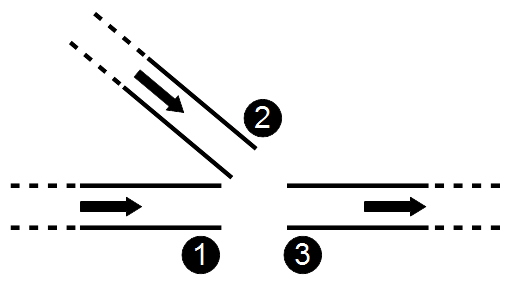
\includegraphics[width=0.8\textwidth]{Figures/Schema_confluent.png}
  \caption{Diagram of a confluence with 3 reaches}
  \label{fig:SchemConf}
 \end{center}
\end{figure}

The junction is bounded by three sections (numbered 1, 2 and 3) located at each end of the associated reaches. These sections are characterized by the hydraulic variables $(Q_1,Z_1)$, $(Q_2,Z_2)$ et $(Q_3,Z_3)$.

We can establish the equations used at the junction by considering the following simple case :
\begin{itemize}
 \item single channel;
 \item steady flow;
 \item velocities along the axis of each branch are identical in the 3 considered sections
% wetted sections such that the velocities along the average axis of the confluence are identical in each branch;
 \item no friction in the junction
 %no friction along the confluent.
\end{itemize}

We can write the Saint-Venant equations along the reach defined by section no. 1 and section no. 3 (the reach corresponding to section no. 2 being treated as lateral contribution - see the previous section \ref{TraitAp})

%axis of the confluent by considering section no. 1 and then section no. 3 .

The continuity equation immediately gives:

\begin{equation}
  Q_3 - Q_1 = Q_2
\end{equation}

The dynamic equation becomes:

\begin{equation}
  V \frac{\partial Q}{\partial x} + g S \frac{\partial}{\partial x} \left ( Z + \beta \frac{V^2}{2 g} \right ) = k q_l V_l
\end{equation}

where $k$ is the coefficient of momentum as indicated in section \ref{TraitAp}.

The key hypothesis is the conservation of velocities along the axis. It means that:

\begin{equation}
  V = k V_l
\end{equation}

and:

\begin{equation}
  \frac{\partial}{\partial x} \left ( \beta \frac{V^2}{2g} \right ) = 0
\end{equation}

We can also write:

\begin{equation}
  \frac{\partial Q}{\partial x} = q_l
\end{equation}

The dynamic equation can therefore be reduced to:

\begin{equation}
  \frac{\partial Z}{\partial x} = 0
\end{equation}

which is equivalent to:

\begin{equation}
  Z_3 = Z_1
\end{equation}

Using a similar reasoning, we consider now the reach defined by sections no. 2 and no. 3, the reach of section no. 1 being treated as inflow, therefore we obtain : $Z_3 = Z_2$.

In summary, the continuity equation gives the conservation of discharges at the junction, and the dynamic equation gives the equality of the water levels.

In a general case, the simple hypotheses used previously are not verified, in particular:
\begin{itemize}
 \item the velocities in each branch are rarely similar;
 \item although friction can often be neglected, singular head losses need to be considered (see the following section).
\end{itemize}

However, the simple relationships obtained here are applied in the subcritical engines. They are the only equations that can be easily implemented in an algorithm.

In practice, the conservation of discharges is always respected, however, the equality of water levels poses a problem. To overcome this difficulty it is usually better to:
\begin{itemize}
 \item place the sections 1-2-3 as close as possible to the junction (to create a \textit{point} junction);
 %choose the closest possible extreme sections (\textit{punctual} confluence);
 \item introduce singular head losses on the branches upstream of the junction to account for the additional dissipation of energy (see the report on confluents in the bibliography and the following section).
\end{itemize}

%...............................................................................
\subsection{Singular head losses}
%...............................................................................

In the dynamic equation, the term $J$ represents the head losses known as linear, which result from the friction on the bottom and the banks. Localised head losses, known as singular head losses, can be produced in the presence of obstacles, rapid variations of sections or junctions.
They are modeled by the mean of a term $J_s$, in addition to $J$ :
\begin{itemize}
 \item for a widening : $J_s = \xi_1 \frac{1}{2 g}(\beta_j V_j - \beta_i V_i)^2$ with :
   \begin{itemize}
     \item the indexes $j$ and $i$ denote respectively the upstream section and the downstream section;
     \item with: $\beta_j V_j < \beta_i V_i$.
   \end{itemize}
 \item for an obstacle placed immediately downstream of the section $j$ : \\ $J_s = \xi_2 \frac{1}{2g} \beta_j V_{j}^2$.
\end{itemize}

where $\xi_1$ and $\xi_2$ are the head losses coefficients.

In the current version of \mascaret{}, the value of $\xi_1$ is a fixed constant equal to 0.3 (based on the litterature), this is valid for gradual widenings (these are automatically taken into account).

The value of $\xi_2$ is set by the user and would often be chosen via a calibration.
A singular head loss modelled with $\xi_2$ needs to be introduced whenever the head loss does not result from a progressive widening
\footnote{This head loss is to be placed at the section $i = j + 1$ : in subcritical flow, with the downstream influencing the upstream, a head loss placed at the section $i$ will increase the head calculated at the section $j = i - 1$, and not reduce the head calculated at the section $i$.}
(sudden narrowing or widening like bridges, etc.).

%...............................................................................
\subsection{Singularities} \label{singu}
%...............................................................................

%...............................................................................
\subsubsection{General principle}
%...............................................................................

The most common singularities are weirs or control dams. However, we will treat this problem more generally by refering to a singularity for any section of the river where the equations of Saint-Venant cannot be applied.

Therefore, in place of the Saint-Venant equations, it is necessary to use specific equations (transfer relationships) that define the influence of the singularity in order to carryout the water line calculations.

We assume that the singularity is located between two computational sections of indices $i$ and $j$ with : $i = j + 1$ (see figure \ref{fig:SchemSing}).

\begin{figure}[H]
 \begin{center}
  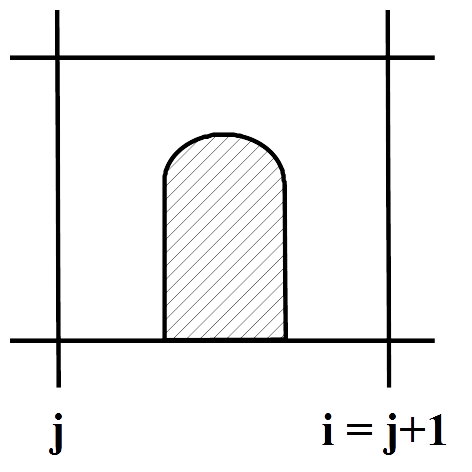
\includegraphics[width=0.5\textwidth]{Figures/Schema_Singularite.png}
  \caption{Diagram of a singularity}
  \label{fig:SchemSing}
 \end{center}
\end{figure}

The continuity equation is reduced to $Q_i = Q_j$, expressing the equality of discharge on each side of the singularity. In unsteady flow, this introduces a slight discrepancy, the volume of water being no longer rigorously conserved. However, this bias is negligible if the distance separating the two calculation sections is \textit{reasonably small}.

The dynamic equation is specific to each type of singularity. Its general expression is : $f(Q, Z_{us},Z_{ds}) = 0$.
The function $f$ is only used in its discretised form in the solution algorithm (see section \ref{MR}).
The equations used for each type of singularity are indicated in the following sections. A summary of the different singularities available in \mascaret{} is shown in section \ref{BilanSing}.

%...............................................................................
\subsubsection{Weirs}
%...............................................................................

In the most general form, the equation for weirs (see the figures hereafter) is of the form : $Q = f(Z_{us},Z_{ds})$, the type of flow (drowned or free flow) is directly integrated in the expression of the function $f$.
$f$ is given in a discretised form with a sufficient series of triplets $(Q,Z_{us},Z_{ds})$.

\begin{itemize}
 \item \textsf{Free flow weir} : the discharge  $Q_d$ depends only on the upstream water level (see figure \ref{fig:Sd});
   \begin{figure}
     \begin{center}
        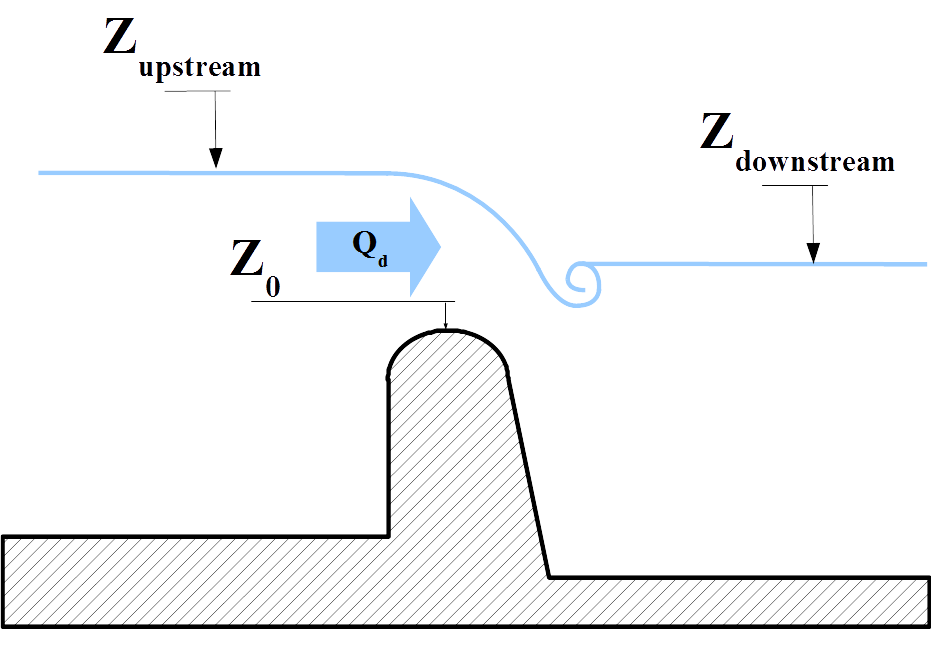
\includegraphics[width=0.8\textwidth]{Figures/Schema_Seuil_Denoye.png}
        \caption{Free flow weir}
        \label{fig:Sd}
     \end{center}
   \end{figure}
   \\
   with $Q = Q_d = m L \sqrt{2g} (Z_{us}-Z_0)^{3/2}$ and :
   \begin{itemize}
     \item $m$ : the discharge coefficient;
     \item $L$ : the width of the weir.
   \end{itemize}

 \item \textsf{Drowned weir}  : the discharge $Q_n$ is influenced by the downstream water level (see figure \ref{fig:Sn});
   \begin{figure}
     \begin{center}
        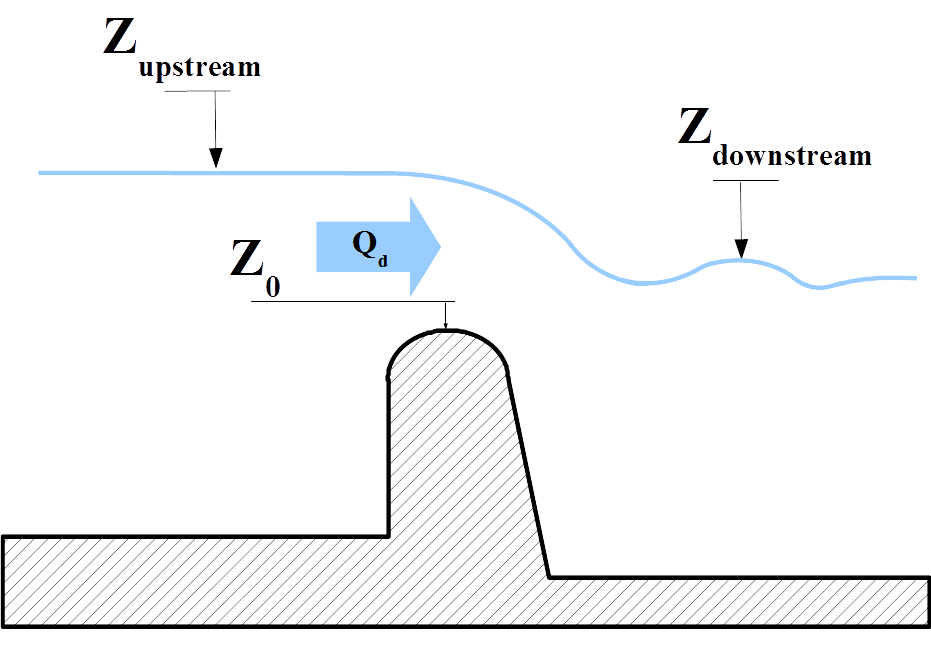
\includegraphics[width=0.8\textwidth]{Figures/Schema_Seuil_Noye.png}
        \caption{Drowned Weir}
        \label{fig:Sn}
     \end{center}
   \end{figure}
   \\
   with $Q = Q_n = C Q_d$ and :
   \begin{itemize}
     \item $C$ : the drowned/free flow coefficient : $C = k \frac{Z_{ds}-Z_{0}}{Z_{us}-Z_0}$;
     \item $k$ : a function to be defined.
   \end{itemize}

\end{itemize}

The discharge law for the weir can also be defined only for free flow conditions (the downstream level does not influence the upstream level), in the form : $Q = f(Z_{us})$, i.e. by indicating a series of pairs $(Q,Z_{us})$.

The flow regime is considered as drowned when : $R = \frac{Z_{ds}-Z_0}{Z_{us}-Z_0}$ is greater than a threshold value $R_0$ (the crest elevation $Z_0$ is a parameter of the weir). An automatic correction is therefore applied : $Q = k(R) f(Z_{us})$. In \mascaret{} the value of the constant $R_0$, and the form of the function $k$, are imposed.

In the current version of \mascaret{}, two types of drowned weirs are distinguished with one relation for sharp-crested weirs and another one for broad-crested weirs (see section \ref{LoiSeuilMinceEpais}). For a broad-crested weir, $Ro$ is equal to 0.8, and $k$ is a parabolic function defined by :

\begin{equation}
  k(R) = -25 R^2 + 40 R -15
\end{equation}
with :
\begin{itemize}
 \item $k(R_0) = 1$;
 \item and $k(1) = 0$.
\end{itemize}


The weir can also be defined by the geometry of the crest, in this case the relation applied for free flow is a spill equation :


\begin{equation}
  Q = m \sqrt{2 g} \sum_{k} L_k (Z_{us} - Z_k)^{3/2}
\end{equation}

where :
\begin{itemize}
 \item $L_k$ is the length of an element of the crest with an elevation $Z_k$;
 \item $m$ is the discharge coefficient (a parameter of the weir).
\end{itemize}

In drowned flow, the discharge correction is identical to that defined above for a broad-crested weir.

%...............................................................................
\subsubsection{Control Structures}
%...............................................................................

The equation for the singularity is simply the imposed upstream water level (varying with time).

%...............................................................................
\subsubsection{Control Sections}
%...............................................................................

The equation for the singularity is a generic relation of the type : $Q = f(Z_{us})$.

A relation : $Q = f(Z_{ds})$ can also be specified but it exists only to enable some specific tests because it does not make physical sense in a subcritical flow regime.

%...............................................................................
\subsection{Surcharged flow}
%...............................................................................

Sections where the flow is surcharged (e.g. under a bridge) do not require a specific treatment in the code.
This is because the cross-sections incorporate a vertical slot with negligible width (the Preissmann slot) at the top of the section. When the cross-section is surcharged, the calculated water level $Z$ is higher than the soffit (top) level of the section, and the pressure $P$ is calculated by means of the relationship : $P = \rho g Z$ .

%These sections are taken into account in the geometry of the profiles. The sections under load must be topped by a vertical slot with negligible width (the Preissmann slot). If the section is indeed under load, the calculated elevation $Z$ will be greater than the obvert level of the section, and will give a value of pressure $P$ by means of the relationship : $P = \rho g Z$ .


%-------------------------------------------------------------------------------
\section{Solution methods} \label{MR}
%-------------------------------------------------------------------------------

%...............................................................................
\subsection{Steady flow in a reach}
%...............................................................................

We consider the typical case of a compound bed.

As we have noted previously, storage cells can be defined but they are not taken into account in the calculation. In this section we consider the case of a single reach; the computation of branched networks is possible for steady subcritical flow and is considered in section \ref{NdPERM}.

%...............................................................................
\subsubsection{Simplification of the equations}
%...............................................................................

The continuity equation is reduced to : $\frac{\partial Q}{\partial x}=q_l$, the discharge is constant along the river, except at the inflows.

The dynamic equation, also called the equation of the water line, takes the form :

\begin{equation}
  \frac{\partial \beta Q V}{x} + g S \left ( \frac{Z}{x} +J + J_s \right )
\end{equation}

It can also be written as :

\begin{equation}
  \frac{\beta}{g} \frac{V}{S} \frac{\partial Q}{\partial x} + \frac{V^2}{2 g} \left ( \frac{\partial \beta}{\partial x} \right ) + \frac{\partial}{\partial x} \left ( \beta \frac{V^2}{2 g} + Z \right ) + J + J_s = 0
\end{equation}

or using the continuity equation :

\begin{equation}
\frac{\beta}{g} \frac{V}{S} q_l + \frac{V^2}{2 g} \left ( \frac{\partial \beta}{\partial x} \right ) + \frac{\partial}{\partial x} \left ( \beta \frac{V^2}{2 g} + Z \right ) + J + J_s = 0
\end{equation}

This equation is discretised along the axis of flow : the discretisation step $\Delta	x$ (separating two consecutive calculation sections) is variable. Its order of magnitude is the width of the river, but in practice it will be related to variability in the sections geometry.

%...............................................................................
\subsubsection{Solving principle}
%...............................................................................

First of all, the continuity equation is solved from the upstream (where the discharge is imposed by the boundary condition) to the downstream, by adding or subtracting the inflows and outflows. Then the calculation of the water level is made, this time going step-by-step from downstream to upstream. For the calculation of a step, we make use of the upstream discharge $Q_1$ and the downstream elevation $Z_2$, and we seek the value of the upstream elevation $Z_1$ (see figure \ref{fig:PRP}).

\begin{figure}[H]
 \begin{center}
  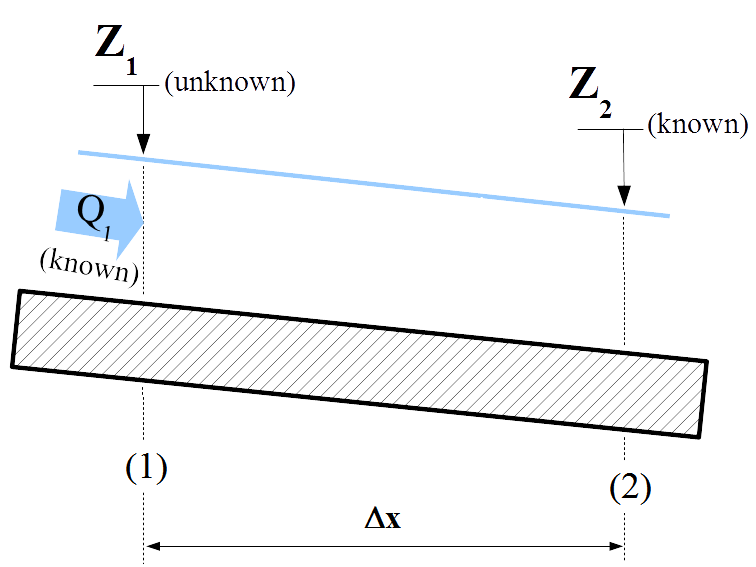
\includegraphics[width=\textwidth]{Figures/Principe_Res_Perm.png}
  \caption{Principle of the steady flow solution}
  \label{fig:PRP}
 \end{center}
\end{figure}

The equation of the water line is discretised between sections 1 and 2 in the following form :

\begin{eqnarray}
  \frac{q_l}{2 g} \left ( \beta_1 \frac{V_1}{S_1} + \beta_2 \frac{V_2}{S_2} \right ) + \frac{V_{1}^2+V_{2}^2}{4 g} \frac{\beta_2 - \beta_1}{\Delta x} + \frac{Z_2-Z_1}{\Delta x} + \nonumber \\
  \frac{1}{\Delta x} \left ( \beta_2 \frac{V_{2}^2}{2 g} - \beta_1 \frac{V_{1}^2}{2 g}  \right ) + \frac{2}{\displaystyle \frac{1}{J_1}+\frac{1}{J_2}} + \nonumber \\
  \frac{\zeta_1}{\Delta x} \frac{\left ( \beta_1 V_1 - \beta_2 V_2 \right ) ^2 }{2 g} + \frac{\zeta_2}{\Delta x} \beta_1 \frac{V_{1}^2}{2 g} = 0
  \label{Dyn5}
\end{eqnarray}

It can also be written :

\begin{equation}
  Z_1 = Z_2 + JDX + JSDX + DXBETA + DXQ + DXV
\end{equation}
where :
\begin{equation}
  JDX = \frac{2}{\displaystyle \frac{1}{J_1} + \frac{1}{J_2}} \Delta x
\end{equation}

\begin{equation}
  JSDX = \frac{1}{2 g} \left ( \zeta_1 \left ( B_1 V_1 - B_2 V_2 \right )^2 + \zeta_2 B_1 V_{1}^2 \right )
\end{equation}

\begin{equation}
  DXBETA = \frac{1}{2 g}(\beta_2 - \beta_1) \left ( \frac{V_{1}^2 + V_{2}^2}{2} \right )
\end{equation}

\begin{equation}
  DXQ = \frac{1}{2 g}(Q_2 - Q_1) \left ( \frac{\beta_1 V_1}{S_1} + \frac{\beta_2 V_2}{S_2} \right )
\end{equation}

and :

\begin{equation}
  DXV = \frac{1}{2 g} ( \beta_2 V_{2}^2 - \beta_1 V_{1}^2 )
\end{equation}

which is equivalent to :

\begin{equation}
  \label{ptfix}
  Z_1 = f(Z_1)
\end{equation}

We must therefore solve the equation (\ref{ptfix}) with the unknown $Z_1$ knowing that there are \textit{a priori} several solutions ; we seek the subcritical solution.

The method involves determining the roots of the function : $\varepsilon = Z_1 - f(Z_1)$.

We start with the approximated solution : $Z_1(0) = Z_2 + J_2 \Delta x$.

We calculate two other approximated solutions with the help of (\ref{ptfix}) : \\
$Z_1(1) = f(Z_2(0))$ hence : $\varepsilon_0 = Z_1(0) - Z_1(1)$ \\
$Z_1(2) = f(Z_1(1))$ hence : $\varepsilon_1 = Z_1(1) - Z_1(2)$

We therefore know two points, $A$ et $B$, of the function $\varepsilon$ (see figure \ref{fig:calsolapproc}) :

\begin{figure}[H]
 \begin{center}
  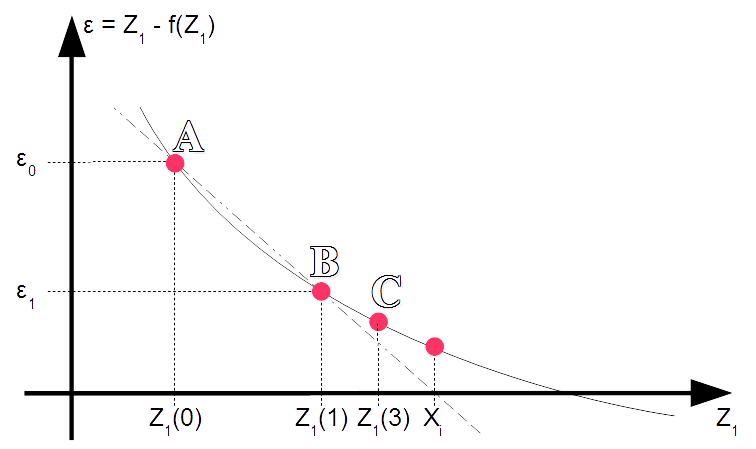
\includegraphics[width=\textwidth]{Figures/Princ_Cal_Sol_Apr.png}
  \caption{Calculation principle for the approximate solution}
  \label{fig:calsolapproc}
 \end{center}
\end{figure}

Knowing these two points, we can use the \textit{secant method} to calculate another approximated solution $X_i$. Experience shows that it is not desirable to use this value, but rather the half-sum of the solutions closest to the axis of $Z_1$, i.e. in figure \ref{fig:calsolapproc} : $Z_{1}(3) = \frac{X_i + Z_{1}(1)}{2}$.

We then calculate $\varepsilon(Z_{1}(3))$, which will give another point on the graph $\varepsilon(Z_1)$, the point $C$. The process resumes from the two points closest to the axis of $Z_1$ (in our case : $B$ et $C$).

We therefore proceed in an iterative manner.

In the case where $\varepsilon(Z_1)$ always keeps the same sign, we stop the calculation when the criteria  $\varepsilon(Z) \leq \Delta$ is satisfied by : $\Delta = 10^{-6}$.

In the case where $\varepsilon(Z)$ changes sign, we initially eliminate, from the two points that are on the same side of the axis of the $Z_1$, the point that is furthest away from it.  We then determine a new approximation from the half-sums of the remaining points.

The calculation is repeated until the stopping criterion is satisfied.

Comment on the solution obtained :
\begin{itemize}
 \item in general, the calculation converges within 10 iterations;
 \item the solution obtained is usually subcritical; however, the following paragraph explains the procedure adopted when this is not the case.
\end{itemize}

\begin{figure}[H]
 \begin{center}
  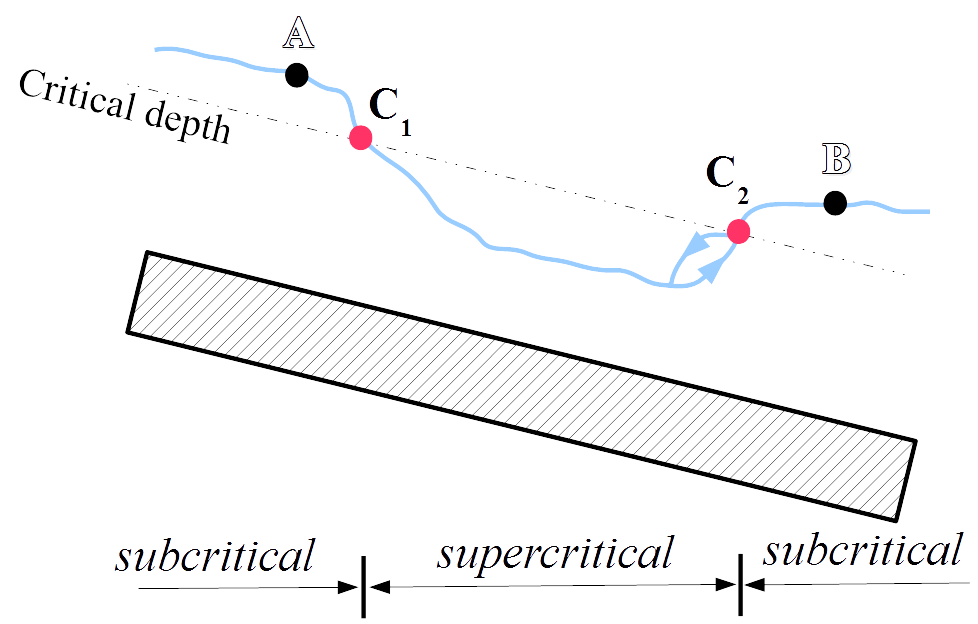
\includegraphics[width=\textwidth]{Figures/Pass_Loc_Tor.png}
  \caption{Diagram of a local passage in supercritical flow}
  \label{fig:PLT}
 \end{center}
\end{figure}


%...............................................................................
\subsubsection{Solving of supercritical zones}
%...............................................................................

When scanning up and down to calculate the subcritical zones, the supercritical zones are also detected (Figure \ref{fig:PLT}). In this case the domain will be swept from upstream to downstream and, for each supercritical zone, a finite-differences discretisation scheme will be applied.

The continuity equation has already been solved at the time of sweeping downstream to upstream. The discharge is known in all points of the discretisation. The equation of the water line, discretised between the section 1 and 2, is similar to equation (\ref{Dyn5}). As opposed to the treatment of subcritical zones, $Z_1$ is known and we look for $Z_2$.

It can also be written :

\begin{equation}
  Z_2 = Z_1 - JDX - JSDX - DXBETA - DXQ - DXV
\end{equation}

As previously, we eventually have to solve the equation :
\begin{equation}
  \label{ptfix1}
  Z_2 = G(Z_2)
\end{equation}

We must therefore solve the equation (\ref{ptfix1}) of unknown $Z_2$ admitting \textit{a priori} several solutions ; we look for the supercritical solution.

The method involves determining the roots of the function : $\varepsilon = Z_2 - f(Z_2)$.
To do that, we do not use the tangent method because the convergence to the supercritical solution would not be assured. The method used is a dichotomy method from the critical level calculated at each point during the calculation of the subcritical zones. The step of the dichotomy is the lesser of :
\begin{itemize}
 \item a $one-hundredth$ of the difference between the elevation of the bottom and the critical water level
 \item and $0.01 m$.
\end{itemize}

The solution is supercritical by construction.

%...............................................................................
\subsubsection{Validity of the hydraulic jump using impulse functions}
%...............................................................................

Once the supercritical zone has been covered, we check that the hydraulic jump is possible from an energy point of view by considering the direction of the increase of the impulse function at the hydraulic jump. It is reminded that impulse functions are maintained through the passage of the hydraulic jump.

\begin{equation}
F_{imp} = \frac{Q^2}{S}+gSh_G \quad \mbox{with : }h_G=\frac{1}{S}\int_0^h(h-y)dy
\end{equation}

If the impulse function at the upstream of the hydraulic jump is higher than the impulse function downstream of the hydraulic jump, the hydraulic jump is moved backward and the flow remains supercritical.

%...............................................................................
\subsection{Unsteady flow in a reach}
%...............................................................................

%...............................................................................
\subsubsection{Principle}
%...............................................................................

We consider the most general case of a compound channel consisting of : low flow channel, high flow channel and storage areas. We consider first the resolution for an unsteady flow for a single reach; the case of branched and meshed networks (possible with the unsteady flow engine) is considered in section \ref{NDRezo}.

We recall the equations governing the water line :
\begin{itemize}
 \item Continuity equation :
   \begin{equation}
     \frac{\partial Q}{\partial x} + L_t \frac{\partial Z}{\partial t} = q_l
   \end{equation}
   where $L_t$ is the total surface width, including the width of the low flow and high flow channels and the storage areas.
  \item Dynamic equation :
    \begin{equation}
      \label{qmv2}
      \frac{\partial Q}{\partial t} + \frac{\partial \beta Q V}{\partial x} + g S \left( \frac{\partial Z}{\partial x} + J + J_s\right) = 0
    \end{equation}
\end{itemize}

This equation (\ref{qmv2}) can also be written by involving the conveyance $D$ :

\begin{equation}
  Q |Q| + D^2 \left ( \frac{\partial Z}{\partial x} +J_s + \frac{1}{S g} \left ( \frac{\partial Q}{\partial t} + \frac{\partial \beta Q V}{\partial x}\right ) \right ) = 0
\end{equation}

These equations are solved with a finite-difference method (see figure \ref{fig:DF}), using an implicit scheme. The discretisation is of the Wendroff type, $\theta$ is the coefficient of implicitation. In a subcritical regime, the scheme is stable when : $\theta > 0.5$ (see \cite{CUNGE64}).

\begin{figure}[H]
 \begin{center}
  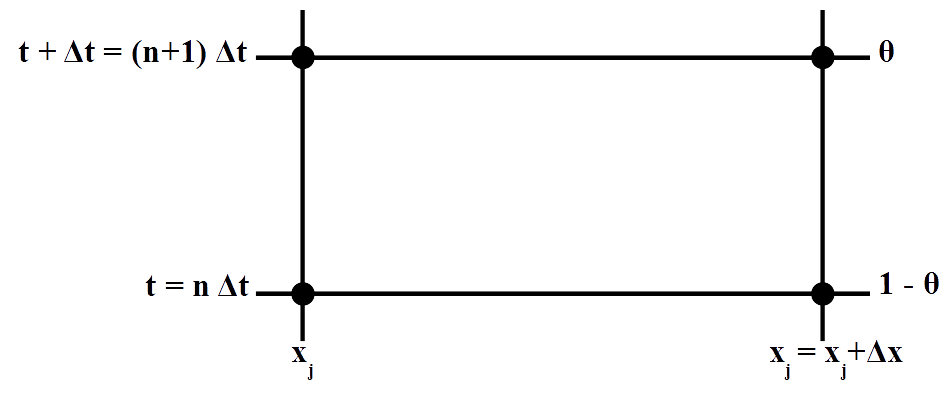
\includegraphics[width=\textwidth]{Figures/Disc_DF.png}
  \caption{Finite differences discretisation}
  \label{fig:DF}
 \end{center}
\end{figure}

We recall the convention : $i = j + 1$. To be rigorous, $\Delta x$ should be written as $\Delta x_j$, the spatial step varying \textit{a priori} in the considered reach.

The derivatives with respect to $x$ and $t$ are calculated (in the first order) in the following way :

\begin{equation}
  \frac{\partial f}{\partial x} = \theta \frac{f_{i}^{n+1}-f_{j}^{n+1}}{\Delta x} + (1-\theta) \frac{f_{i}^n - f_{j}^n}{\Delta x}
\end{equation}

\begin{equation}
  \frac{\partial f}{\partial t} = \frac{1}{2} \left ( \frac{f_{i}^{n+1} - f_{i}^n}{\Delta t} + \frac{f_{j}^{n+1} - f_{j}^n}{\Delta t} \right )
\end{equation}

The functions that occur without a derivative are evaluated by :

\begin{equation}
  f = \theta \frac{f_{i}^{n+1} + f_{j}^{n+1}}{2} + (1 - \theta) \frac{f_{i}^n + f_{j}^n}{2}
\end{equation}

%...............................................................................
\subsubsection{Discretised equations}
%...............................................................................

The discretised equations are written as follows :

\begin{itemize}
  \item Continuity equation :
  \begin{eqnarray}
    (1 - \theta) \frac{Q_{i}^n - Q_{j}^n}{\Delta x} + \theta \frac{Q_{i}^{n+1} - Q_{j}^{n+1}}{\Delta x} + \frac{1}{2} \left ( L_{t_i}^n + L_{t_j}^n \right ) \nonumber \\
    \times \frac{1}{2} \left ( \frac{Z_{i}^{n+1} - Z_{i}^n}{\Delta t} + \frac{Z_{j}^{n+1} - Z_{j}^n}{\Delta t} \right ) = q_{l_j}^{n+1}
  \end{eqnarray}

  \item Dynamic equation :
  \begin{eqnarray}
    \left ( \frac{1 - \theta }{2} \right ) \left ( Q_{j}^{n^2} + Q_{i}^{n^2} \right ) + \frac{\theta}{2} \left ( Q_{j}^{n+1^2} + Q_{i}^{n+1^2} \right ) \nonumber \\
    + \left ( \frac{1 - \theta}{2} \left ( D_{i}^{n^2} + D_{j}^{n^2} \right ) + \frac{\theta}{2} \left ( D_{i}^{n^2} + D_{j}^{n+1^2} \right ) \right ) \nonumber \\
    \times \Bigg \{ (1 - \theta) \frac{Z_{i}^n - Z_{j}^n}{\Delta x} + \theta \frac{Z_{i}^{n+1} - Z_{j}^{n+1}}{\Delta x} + J_{s}(i) + J_{s}(j) \nonumber \\
    + \left ( \frac{1 - \theta}{2 g} \left ( \left ( \frac{1}{S} \right )_{i}^n + \left ( \frac{1}{S} \right )_{j}^n \right ) + \frac{\theta}{2 g} \left ( \left ( \frac{1}{S} \right )_{i}^{n+1} + \left ( \frac{1}{S} \right )_{j}^{n+1} \right ) \right ) \nonumber \\
    \times \Bigg [ \frac{1}{2 \Delta t}(Q_{i}^{n+1}-Q_{i}^n+Q_{j}^{n+1}-Q_{j}^n) + \frac{\theta}{\Delta x} \left ( \beta_{i}^n \frac{Q_{i}^{n+1^2}}{S_{i}^{n+1}}-\beta_{j}^n \frac{Q_{j}^{n+1^2}}{S_{j}^{n+1}} \right ) \nonumber \\
    + \frac{1-\theta}{\Delta x} \left ( \beta_{i}^n \frac{Q_{i}^{n^2}}{S_{i}^{n}}-\beta_{j}^n \frac{Q_{j}^{n^2}}{S_{j}^{n}} \right ) \Bigg ] \Bigg \} = 0
  \end{eqnarray}
\end{itemize}

We introduce the following variables :

\begin{equation}
 \left \lbrace
  \begin{array}{l}
    \Delta Q_j = Q_{j}^{n+1} - Q_{j}^n \\
    \Delta Q_i = Q_{i}^{n+1} - Q_{i}^n \\
    \Delta Z_j = Z_{j}^{n+1} - Z_{j}^n \\
    \Delta Z_i = Z_{i}^{n+1} - Z_{i}^n
  \end{array}
 \right.
\end{equation}

and, after linearisation (i.e. preserving only the first order terms in $\Delta Z$ and $\Delta Q$) we get :

\begin{itemize}
 \item for the continuity equation :
  \begin{equation}
   \label{CONT}
   \boxed{
     G \Delta Q_i + H \Delta Z_i = I \Delta Q_j + J \Delta Z_j + K
   }
  \end{equation}
  with :
  \begin{equation}
   \label{CONT1}
   G = \theta
  \end{equation}
  \begin{equation}
    \label{CONT2}
   I = G
  \end{equation}
  \begin{equation}
    \label{CONT3}
   H = \frac{\Delta x}{4 \Delta t} ( L_{t_j}^n + L_{t_i}^n )
  \end{equation}
  \begin{equation}
    \label{CONT4}
   J = -H
  \end{equation}
   \begin{equation}
   \label{CONT5}
   K = Q_{j}^n - Q_{i}^n + q_{l_i}^{n+1}
  \end{equation}

 \item and for the dynamic equation :
  \begin{equation}
   \label{DYN}
   \boxed{
     L \Delta Q_i + M \Delta Z_i = N \Delta Q_j + O \Delta Z_j + P
   }
  \end{equation}
  with :
  \begin{equation}
    \label{DYN1}
   L = B_2 + C_1 H_1 ( E_2 + F_2 )
  \end{equation}
  \begin{equation}
    \label{DYN2}
   M = C_1 ( D_4 + H_1 F_4 + H_4 F_1 ) + C_4 ( D_1 + H_1 F_1 )
  \end{equation}
   \begin{equation}
    \label{DYN3}
   N = -B_3 - C_1 H_1 ( E_3 + F_3 )
  \end{equation}
  \begin{equation}
     \label{DYN4}
   O = -C_1 ( D_5 + H_1 F_5 + H_5 F_1 ) - C_5 ( D_1 + H_1 F_1 )
  \end{equation}
  \begin{equation}
   \label{DYN5}
   P = -B_1 - C_1 ( D_1 + H_1 F_1 )
  \end{equation}
\end{itemize}

knowing that the various terms of the dynamic equation have been linearised in the following way (the non-indexed variables correspond to the time steps $n$) :

\begin{equation}
 Q |Q| = B_1 + B_2 \Delta Q_i + B_3 \Delta Q_j
\end{equation}

\begin{equation}
 B_1 = \frac{1}{2} ( Q_{i}^2 sign(Q_i) + Q_{j}^2 sign(Q_j) )
\end{equation}

\begin{equation}
 B_2 = \theta |Q_i|
\end{equation}

\begin{equation}
 B_3 = \theta |Q_j|
\end{equation}

\begin{itemize}
 \item[*]
  \begin{equation}
   D^2 = C_1 + C_4 \Delta Z_i + C_5 \Delta Z_j
  \end{equation}
  \begin{equation}
   C_1 = \frac{1}{2} ( D_{i}^2 + D_{j}^2 )
  \end{equation}
  \begin{equation}
   C_4 = \theta D_i ( \alpha_{m_i} + \alpha_{M_i} )
  \end{equation}
  \begin{equation}
   C_5 = \theta D_j ( \alpha_{m_j} + \alpha_{M_j} )
  \end{equation}
  \begin{equation}
   \alpha_{m_i} = \frac{K_m R_{m}^{2/3}}{3} \left ( 5 L_m -2 R_m \frac{\partial P_m}{\partial z} \right )_i
  \end{equation}
   \begin{equation}
   \alpha_{m_j} = \frac{K_m R_{m}^{2/3}}{3} \left ( 5 L_m -2 R_m \frac{\partial P_m}{\partial z} \right )_j
  \end{equation}
  \begin{equation}
    \alpha_{M_i} = \frac{K_M R_{M}^{2/3}}{3} \left ( 5 L_M -2 R_M \frac{\partial P_M}{\partial z} \right )_i
  \end{equation}
  \begin{equation}
    \alpha_{M_j} = \frac{K_M R_{M}^{2/3}}{3} \left ( 5 L_M -2 R_M \frac{\partial P_M}{\partial z} \right )_j
  \end{equation}
  \begin{equation}
    K_{m}' = A K_m
  \end{equation}
  \begin{equation}
    K_{M}' = \sqrt{1 + \frac{S_m}{S_M} (1-A^2)} K_M
  \end{equation}
 \item[*]
  \begin{equation}
    \frac{\partial Z}{\partial x} + J_{s}(i) + J_{s}(j) = D_1 + D_4 \Delta Z_i + D_5 \Delta Z_j
  \end{equation}
  \begin{equation}
     D_1 = \frac{Z_i - Z_j}{\Delta x} + J_{s}(i) + J_{s}(j)
  \end{equation}
  \begin{equation}
    D_4 = \frac{\theta}{\Delta x}
  \end{equation}
    \begin{equation}
    D_5 = \frac{\theta}{\Delta x}
  \end{equation}
 \item[*]
   \begin{equation}
     \frac{\partial Q}{\partial t} = E_2 \Delta Q_i + E_3 \Delta Q_j
   \end{equation}
   \begin{equation}
     E_2 = \frac{1}{2 \Delta t}
   \end{equation}
   \begin{equation}
     E_3 = \frac{1}{2 \Delta t}
   \end{equation}
 \item[*]
   \begin{equation}
    \frac{\partial}{\partial x} \left ( \beta \frac{Q^2}{S} \right ) = F_1 + F_2 \Delta Q_i + F_3 \Delta Q_j + F_4 \Delta Z_i + F_5 \Delta Z_j
   \end{equation}
   \begin{equation}
     F_1 = \frac{1}{\Delta x} ( \beta_i V_i Q_i - \beta_j V_j Q_j )
   \end{equation}
   \begin{equation}
     F_2 = \frac{2 \theta}{\Delta x} \beta_i V_i
   \end{equation}
   \begin{equation}
     F_3 = -\frac{2 \theta}{\Delta x} \beta_j V_j
   \end{equation}
   \begin{equation}
     F_4 = - \frac{\theta}{\Delta x} \beta_i V_{i}^2 L_{t_i}
   \end{equation}
   \begin{equation}
     F_5 = \frac{\theta}{\Delta x} \beta_j V_{j^2} L_{t_j}
   \end{equation}
 \item[*]
   \begin{equation}
    \frac{1}{S g} = H_1 + H_4 \Delta Z_i + H_5 \Delta Z_j
   \end{equation}
   \begin{equation}
     H_1 = \frac{1}{2 g} \left ( \frac{1}{S_i} + \frac{1}{S_j} \right )
   \end{equation}
   \begin{equation}
     H_4 = - \frac{\theta}{2 g} \frac{L_{t_i}}{S_{i}^2}
   \end{equation}
   \begin{equation}
     H_5 = - \frac{\theta}{2 g} \frac{L_{t_j}}{S_{j}^2}
   \end{equation}
\end{itemize}

%...............................................................................
\subsubsection{Solving the discretised equations}
%...............................................................................

The equations (\ref{CONT}) and (\ref{DYN}) lead directly to the establishment of a matrix system :

\begin{equation}
 \label{systm}
 \left(
    \begin{array}{cc}
       G & H \\
       L & M
    \end{array}
 \right)
 \left(
    \begin{array}{c}
       \Delta Q_i \\
       \Delta Z_i
    \end{array}
 \right)
 =
  \left(
    \begin{array}{cc}
       I & J \\
       N & O
    \end{array}
 \right)
 \left(
    \begin{array}{c}
       \Delta Q_j \\
       \Delta Z_j
    \end{array}
 \right)
 +
 \left(
    \begin{array}{c}
       K \\
       P
    \end{array}
 \right)
\end{equation}

where $G$,$H$,$I$,$J$,$K$,$L$,$M$,$N$,$O$ et $P$ are macro-coefficients, their expression
depend on the control variables, the state variables and the parameters of the model (\ref{CONT1}-\ref{CONT5}) (\ref{DYN1}-\ref{DYN5}).

In the case of a single reach, the boundary conditions at the upstream and downstream ends mean that $\Delta Q_1$ and $\Delta Z_n$ are no longer unknowns, $n$ being the number of calculation sections. This corresponds to an imposed discharge at the upstream end and an imposed water level at the downstream end. The system (\ref{systm}) therefore comprises $2n-2$ equations and as many unknowns. It is expressed in the general form :

\begin{equation}
 \label{eq1}
 A.x = b
\end{equation}
where :
\begin{itemize}
 \item the vector $x$ of the unknowns, is the solution of the variations of elevation and discharge at each one of the $n$ calculation sections in the network of reaches :
   \begin{equation}
      x = \left(
            \begin{array}{c}
               \Delta Z_1\\
               \Delta Q_2\\
               \Delta Z_2\\
               \Delta Q_3\\
               \Delta Z_3\\
               \vdots\\
               \Delta Z_{n-1}\\
               \Delta Q_{n}
            \end{array}
          \right)
   \end{equation}
 \item in the simple case of a single reach, the matrix $A$ is an asymmetric band matrix :
   \begin{equation}
     \label{eq3}
     A = \left(
         \begin{array}{cccccccccccc}
          -J & G & H & & & & & & & & & \\
          -O & L & M & & & & & & & & & \\
             & -I & -J & G & H & & & & & & & \\
             & -N & -O & L & M & & & &  & 0 & & \\
             & & & -I & -J & G & H & & & & & \\
             & & & -N & -O & L & M & & & & & \\
             & & & & & & & .... & & & & \\
             & & & & & & & & .... & & & \\
             & 0 & & & & & & & & .... & & \\
             & & & & & & & & & & .... & \\
             & & & & & & & & & -I & -J & G \\
             & & & & & & & & & -N & -O & L \\
         \end{array}
         \right)
   \end{equation}
 \item $b$ is the vector of the second member of the equation :
   \begin{equation}
      \label{eq2}
      b = \left(
            \begin{array}{c}
               K\\
               P\\
               K\\
               P\\
               \vdots\\
               K\\
               P
            \end{array}
          \right)
   \end{equation}
\end{itemize}

The various macro-coefficients $G, H, I, J, K, L, M, N, O\ et\ P$ are calculated at each time step.

The matrix $A$ presents two important characteristics : it is a diagonally-dominant band matrix and is very sparse. It is then possible to use a specialised solver to solve (\ref{eq1}).

Two linear solvers are implemented in the code \REZO{}.

\begin{itemize}
  \item the first one is the band solver \texttt{DGBSV} of the \texttt{LAPACK}\footnote{http://www.netlib.org/lapack/} numerical library. This solver is the default one when the problem deals with only one reach with no storage cell;
  \item the second is a sparse solver written in %\textit{Fortran77} \texttt{Y12M}\footnote{http://www.netlib.org/y12m/}. This program was developed at %the beginning of the 1980s \cite{ZLATEV81}. It benefits from a robustness and performance proven for %the size of problems that the code \REZO{} is used for.\texttt{Y12M} is a direct solver with numerical pivoting to preserve the stability of the calculation, and the sparseness of the matrix factorised as an $L.U$ product. Using this solver is particularly simple and light because of :
\begin{itemize}
 \item the call of a single routine and a reduced number of sources;
 \item the internal management of the renumbering to preserve the sparseness (a choice of the pivot, with a criterion of fill minimization);
 \item the matrix chaining is filled using the coordinates format $(i,j)$ for each non-zero element that is present in the line $i$ and column $j$.
\end{itemize}

\end{itemize}

The solving of a sub-critical and unsteady problem by the \REZO{} code follows the algorithmic stages described in Figure \ref{fig:Etap}.

\begin{figure}[H]
 \begin{center}
  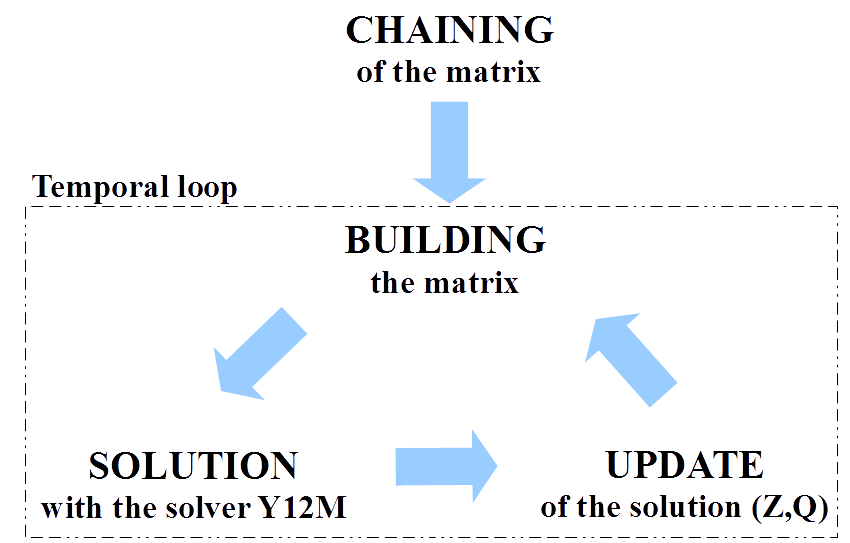
\includegraphics[width=0.8\textwidth]{Figures/AlgoRezo.png}
  \caption{\REZO{} algorithm}
  \label{fig:Etap}
 \end{center}
\end{figure}

Before starting the time-based simulation, the chaining of the matrix must be determined, starting with the schematic of the network. This calculation is carried out only once because the connectivity of the network does not change with time.

The time loop consists of three phases :
\begin{itemize}
 \item a calculation of the macro-coefficients $G, H, I, J, K, L, M, N, O\ and\ P$ and their assembly in the matrix $A$ and the second member of the equation $b$;
 \item the use of the direct solver \texttt{Y12M} or \texttt{DGBSV }for solving the system (\ref{eq1}) and determine the solution of the elevation and discharge variations $(\Delta Z_i,\Delta Q_i)$ in each section $i$;
 \item an update of the water line for the current time $t_k$ :
  \begin{equation}
   \forall i \in 1...n
   \left \lbrace
  \begin{array}{l}
    Q_{i}^{k} = Q_{i}^{k-1} + \Delta Q_i \\
    \\
    Z_{i}^{k} = Z_{i}^{k-1} + \Delta Z_i
  \end{array}
 \right.
  \end{equation}
\end{itemize}

%...............................................................................
\subsection{Treatment of junctions in a steady subcritical regime} \label{NdPERM}
%...............................................................................

%...............................................................................
\subsubsection{Reminder}
%...............................................................................

The equations solved at the junctions are :
\begin{itemize}
 \item the continuity of discharges;
 \item the equality of elevations in each branch (see the justification in section \ref{TrNd}).
\end{itemize}

Therefore a junction does not add any additional unknown : the unknowns to be calculated are the unknowns $(Z,Q)$ of the computational sections forming this junction. Therefore, in the example below (figure \ref{fig:SchNd}):

\begin{figure}[H]
 \begin{center}
  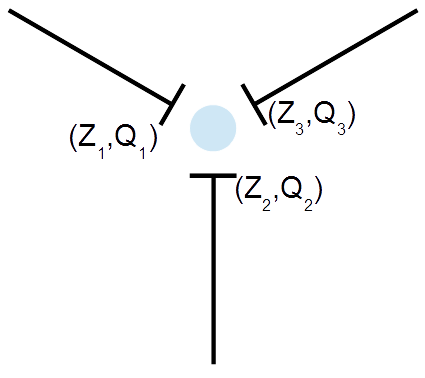
\includegraphics[width=0.8\textwidth]{Figures/Schema_noeud.png}
  \caption{Example of a junction with three branches}
  \label{fig:SchNd}
 \end{center}
\end{figure}

The unknowns are $(Z_1,Q_1)$, $(Z_2,Q_2)$ and $(Z_3,Q_3)$ and the equations of the junction are :
\begin{itemize}
 \item the distribution of discharges : $Q_1 + Q_2 + Q_3 = 0$;
 \item the equality of the water levels : $Z_1 = Z_2 = Z_3$.
\end{itemize}

We can easily verify that these relationships are sufficient to determine the values of $(Z,Q)$ throughout the considered network.

If we call :
\begin{itemize}
 \item the total number of computational sections to be processed (i.e. the sum of the calculation sections in all of the branches) : $im$;
 \item the number of reaches : $nbreach$;
 \item the number of free ends : $nblimi$.
\end{itemize}

then for the whole network we can write $(im-nbreach)$ continuity equations and as many discrete dynamic equations of Saint-Venant.

The unknowns are the $(\Delta Q,\Delta Z)$ of the computation sections, and so there are $2 im$ unknowns.

The boundary conditions are known at the extremities, which gives $nblimi$ additional relationships.

For all of the nodes we can write :
\begin{itemize}
 \item[*] $nbnode$ discharge conservation equations;
 \item[*] $(2nbreach-nblimi) - nbnode$ equal elevation equations.
\end{itemize}

This is because $(2nbreach - nblimi)$ represents the number of branch extremities connecting to a junction (each reach should be counted twice except those that have a free end). At each junction, if $k$ branches are connected, there are only $k-1$ equations that come from the equality of elevations. It is therefore necessary to subtract $nbnode$ from $2nbreach - nblimi$.

Finally, we have : \\
$2 (im - nbreach) + nblimi + nbnode + (2 nbreach - nblimi) - nbnode$
$= 2 im$ equations for $2 im$ unknowns.

%...............................................................................
\subsubsection{Principle}
%...............................................................................

The algorithm presented here is valid regardless of the network (branched or meshed) provided the following conditions are met :
\begin{itemize}
 \item the direction of flow is known \textit{a priori} in each reach;
 \item for all extremities, the boundary condition is:
   \begin{itemize}
     \item the discharge, if it is an upstream end;
     \item the elevation, if it is a downstream end.
    \end{itemize}
\end{itemize}

In practice, there is a risk that this algorithm becomes very time consuming if the network is complex (i.e. interconnected distributaries, see below). In that case, it would be better to use the unsteady subcritical engine (see the following section), starting with a simple initial water line, and choosing the boundary conditions so as to converge towards a stationary state corresponding to the water line being sought.

Before presenting the algorithm, it is useful to make the following observation. The problem is very simple if the network is only comprised of confluences because the discharge is calculated at every point of the domain descending from the upstream ends ; therefore it suffices to calculate the elevation of the water line by following the reverse path (i.e. gradually moving towards the upstream ends), using the same procedure as for a reach. At each node, the equality of the elevations can be imposed without difficulty.

The critical problem is therefore to calculate the distribution of discharge at a junction. The solution used here is an iterative method that is explained in the following paragraph. This means that the general algorithm is itself iterative : the iterations are interlinked in the same way as the distributaries (see figures \ref{fig:AlgSP} and \ref{fig:ExSP}). We can further specify that :
\begin{itemize}
 \item \textit{to descend a reach} means to calculate the discharge at each successive computational section, working from upstream to downstream;
 \item \textit{to ascend a reach} means to calculate the elevation at each successive computational section, working from downstream to upstream.
\end{itemize}

Figure \ref{fig:AlgSP} presents the solution algorithm, while figure \ref{fig:ExSP} illustrates the example of a meshed network including two interlinked distributaries. This example could be considered as representative of the more complex cases that can be computed within a reasonable time by this algorithm. Beyond that, as indicated previously, it is recommended that the \REZO{} code for unsteady flows is used.

\begin{figure}[H]
 \begin{center}
  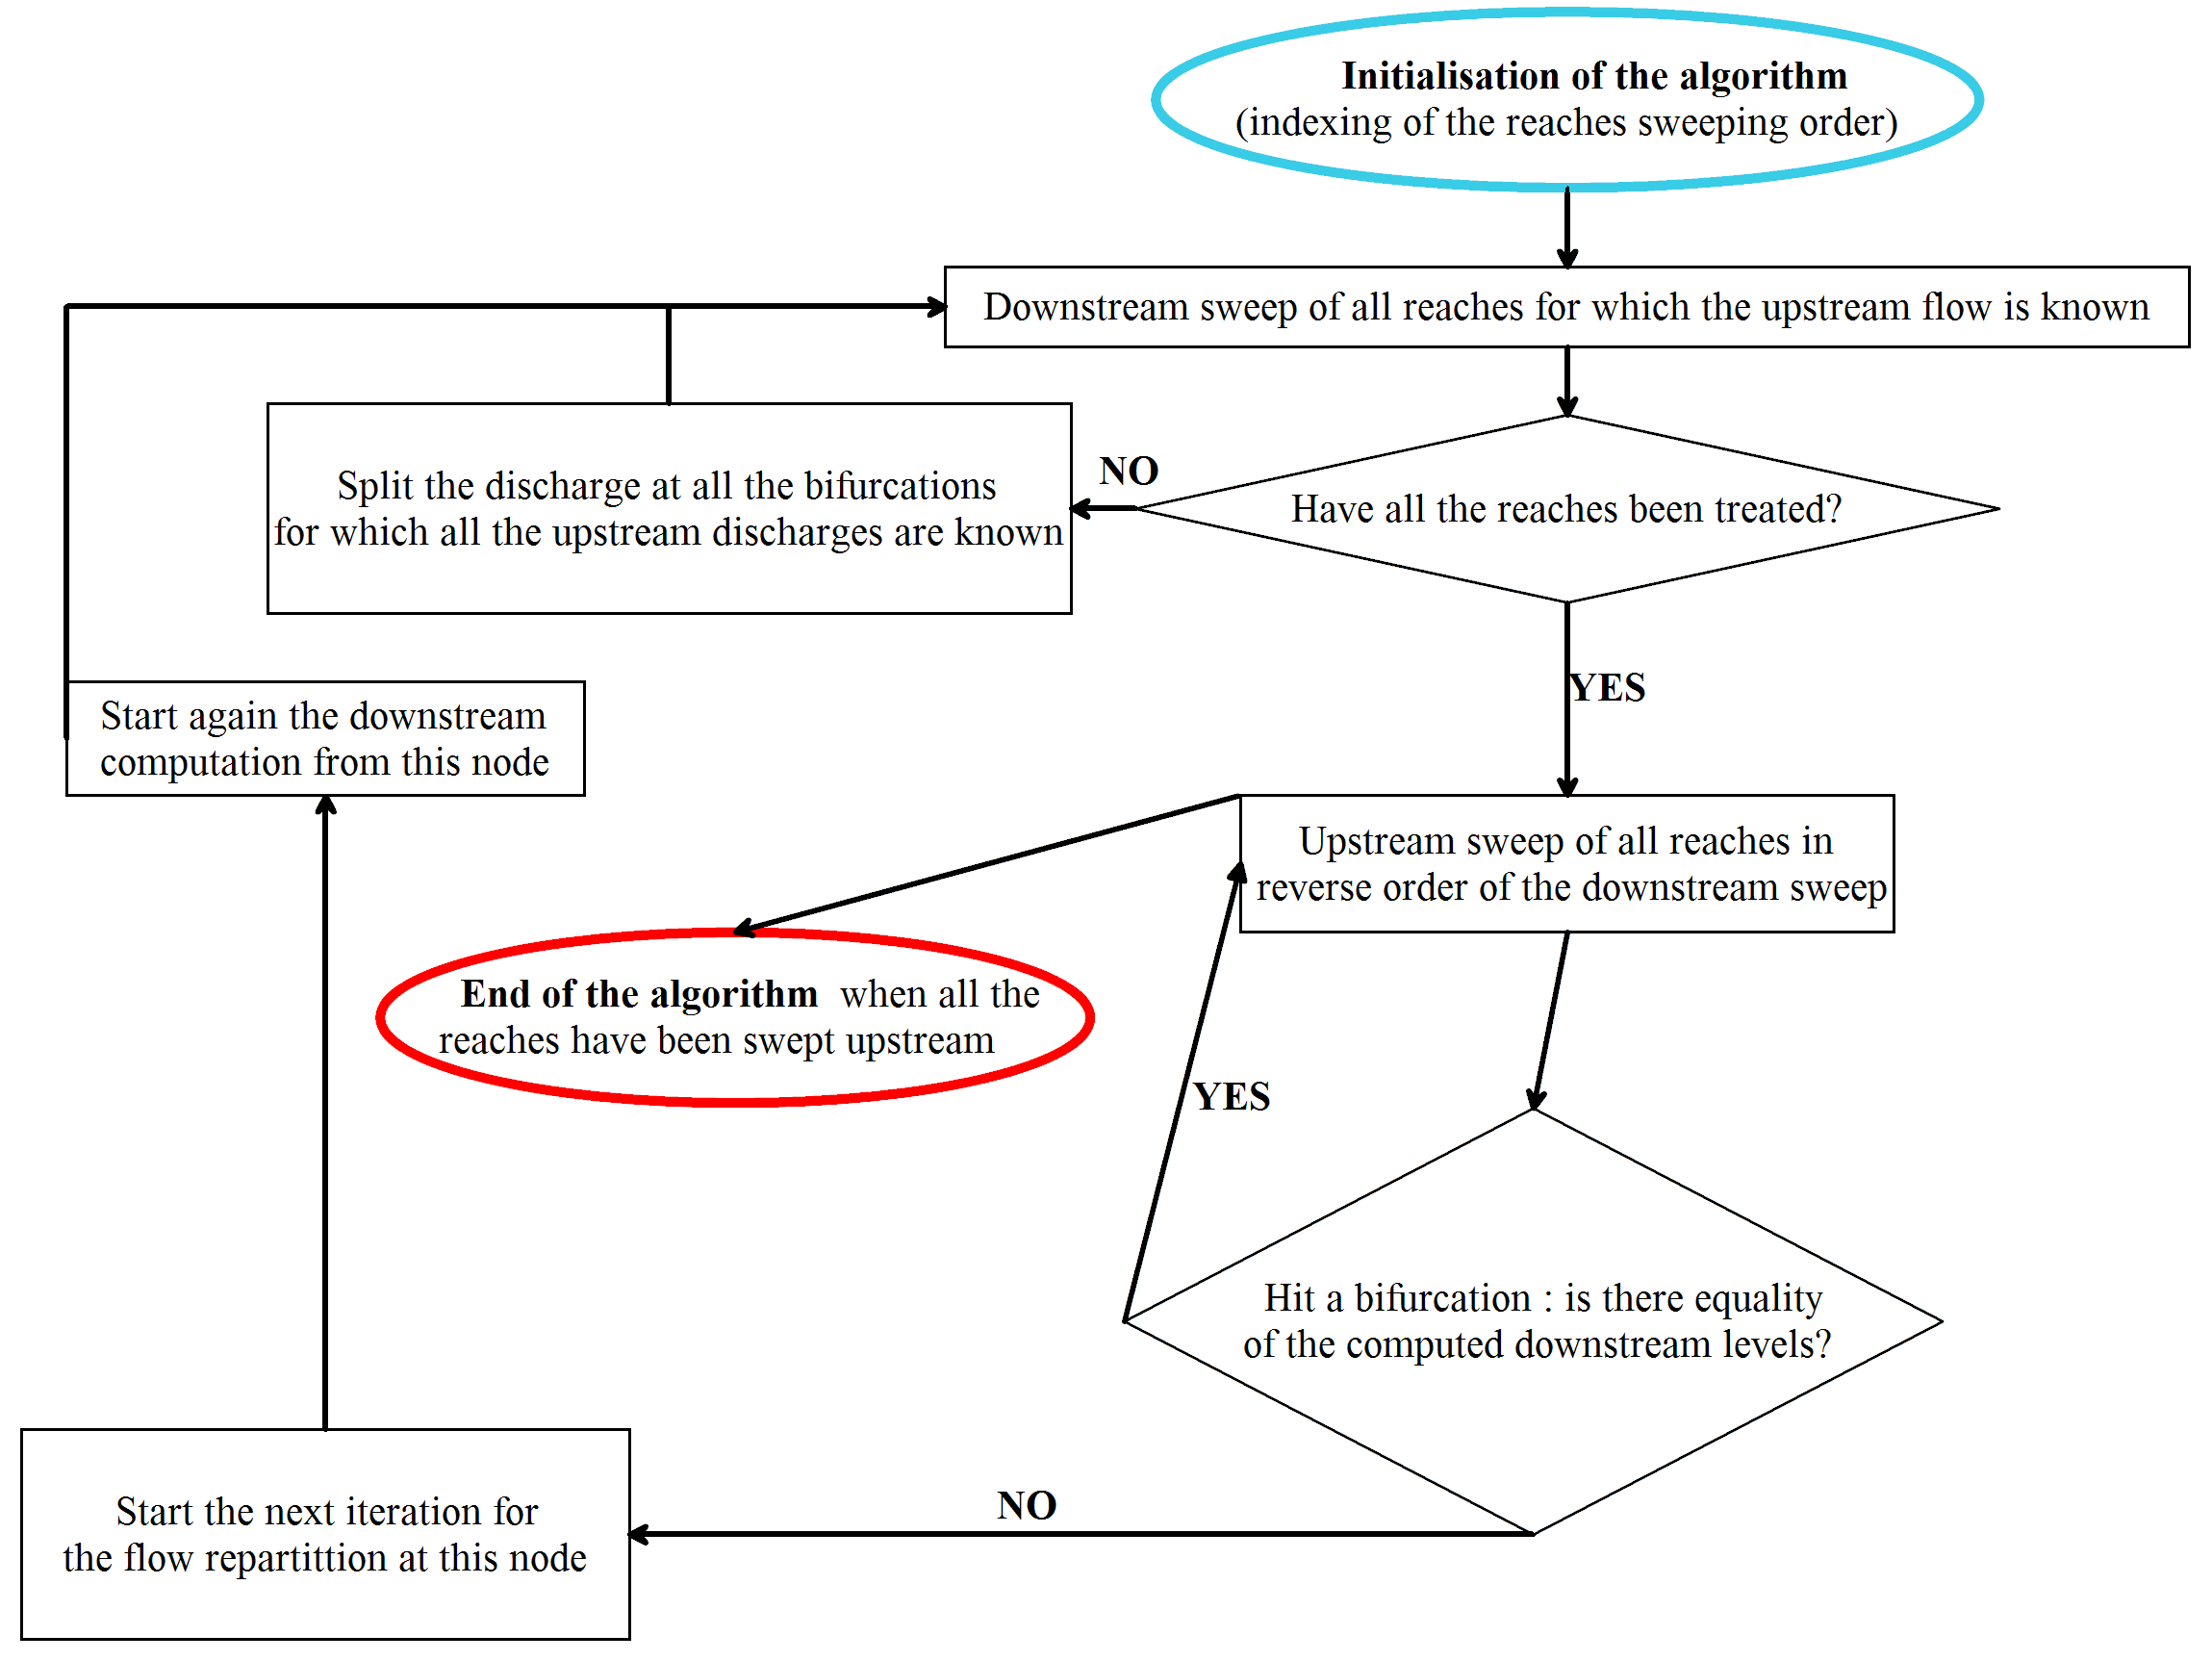
\includegraphics[width=\textwidth]{Figures/Algorithm_SARAP.png}
  \caption{Solution algorithm for a steady state network}
  \label{fig:AlgSP}
 \end{center}
\end{figure}

\begin{figure}[H]
 \begin{center}
  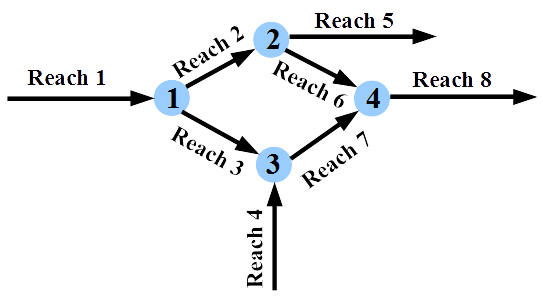
\includegraphics[width=\textwidth]{Figures/Ex_Res_SARAP.png}
  \caption{Example of a network for a steady state calculation}
  \label{fig:ExSP}
 \end{center}
\end{figure}

\textsc{\textbf{algorithm} (see figure \ref{fig:ExSP}) :}
\begin{itemize}
 \item[*] Descend Reach 1
 \item[*] Descend Reach 4
 \item[*] $n = 1$
 \item[*] \textbf{(1)} Spread the discharge at node 1 (iteration $n$)
 \begin{itemize}
  \item Descend Reach 2
  \item Descend Reach 3
  \item Descend Reach 7
  \item $p = 1$
  \item \textbf{(2)} Spread the discharge at node 2 (iteration $n.p$)
  \begin{itemize}
   \item Descend Reach 5
   \item Descend Reach 6
   \item Descend Reach 8
  \end{itemize}
  -----------------------------
  \begin{itemize}
   \item Ascend Reach 8
   \item Ascend Reach 6
   \item Ascend Reach 5
   \item Equality of the downstream elevations at node 2?
   \begin{itemize}
    \item if no : $p = p + 1$, go back to step \textbf{(2)}
    \item if yes : continue
   \end{itemize}
  \end{itemize}
  \item Ascend Reach 7
  \item Ascend Reach 3
  \item Ascend Reach 2
  \item Equality of the downstream elevations at node 1?
  \begin{itemize}
    \item if no : $n = n + 1$, go back to step \textbf{(1)}
    \item if yes : continue
   \end{itemize}
  \end{itemize}
 \item Ascend Reach 4
 \item Ascend Reach 1
\end{itemize}

%...............................................................................
\subsubsection{Discharge distribution in a diffluence (bifurcation)}
%...............................................................................

\textbf{First Iteration}

The discharge distribution needs to verify :

\begin{equation}
  Q_{us} + \sum_{i=1}^{n_{ds}} Q_i
\end{equation}
where $n_{ds}$ is the number of downstream branches.

\begin{equation}
  Q_i = D_i J_{i}^{1/2}
\end{equation}

The solution used here is the equality of the slopes of the total head line :

\begin{equation}
  J_i = J = \left ( \frac{Q_i}{D_i}^2 \right )
\end{equation}

or :

\begin{equation}
  \frac{Q_i}{D_i} = \frac{Q_j}{D_j} = ct = J^{1/2}
\end{equation}

Substituting this into the continuity equations leads to:

\begin{equation}
 \frac{Q_{us}}{J^{1/2}} = \sum_{i=1}^{n_{ds}} D_i
\end{equation}

The sum of the conveyances depends only on the geometry and the roughness of the downstream reaches and is a function of the elevation that, in general, increases monotonously.

For a given value of $J$, it is possible to calculate an elevation satisfying this relationship, and then calculate the $D_j$ and then the  $Q_j$ for that elevation.

In the current version of \mascaret{}, the approach used for the first iteration is to take $J$ as the average of the slopes of the bottom of the downstream branches.

\textbf{Subsequent iterations}

The problem to solve is determining the best corrections of discharge to make (compared to the distribution chosen for the previous iteration), in order to come as close as possible to the equality of elevations at the first sections of the downstream reaches.

The approach is to determine the correction of discharge by assuming the slopes of the energy lines $J$ (equal to those of the preceding iteration) in order to tend towards the equality of the elevations (while still respecting the continuity of the discharges).

For each of the first sections of the downstream branches, we can write (for a given elevation) :

\begin{equation}
 Q_{i}^2 = J_i D_{i}^2
\end{equation}
or :
\begin{equation}
 Q_{i} = J_{i}^{1/2} D_{i}
\end{equation}
the index $i$ corresponds to the number of the downstream branch.

By differentiating between the iterations $n$ and $n+1$, we get :
%and by developing the term $J_{i}^{1/2}$

\begin{equation}
 \label{i1}
 \delta Q_i = ( J_{i}^{1/2} )_n \left ( \frac{\partial D_i}{\partial Z_i} \right )_n \delta Z_i
\end{equation}
where $n$ denotes the number of the current iteration,

with :

\begin{equation}
 ( J_{i}^{1/2} )_n = \left ( \frac{Q_i}{D_i} \right )_n
\end{equation}

where : $\delta Q_i = Q_{i}^{n+1} - Q_{i}^{n}$
and : $\delta Z_i = Z_{i}^{n+1} - Z_{i}^{n}$

If $n_{ds}$ is the number of downstream branches then the continuity of the discharges is written  :
\begin{equation}
  Q_{us} = \sum_{i=1}^{n_{ds}} Q_i
\end{equation}
where :

\begin{equation}
 \label{i2}
 \sum_{i=1}^{n_{ds}} \delta Q_i = 0
\end{equation}

The correction of discharge is done to tend towards the equality of the elevations at the junction. We therefore want :

\begin{equation}
 Z_{i}^{n+1} = ct = Z
\end{equation}
which gives :

\begin{equation}
 \label{i3}
  \delta Z_i = Z - Z_{i}^n
\end{equation}
where the $Z_{i}^n$ are the results of the previous iteration.

So we have :
\begin{itemize}
 \item $n_{ds}$ relationships (\ref{i1});
 \item 1 relationship (\ref{i2});
 \item $n_{ds}$ relationships (\ref{i3}).
\end{itemize}
and so there are $2n_{ds}+1$ relationships for $2n_{ds}+1$ unknowns ($\delta Q_i$,$\delta Z_i$ and $Z$).

\begin{equation}
 \left \lbrace
  \begin{array}{l}
    \delta Z_i = Z - Z_{i}^n \\
    \sum_{i=1}^{n_{ds}} \delta Q_i = 0 \\
    \delta Q_i = \left ( \frac{Q_i}{D_i} \right )_n \left ( \frac{\partial D_i}{\partial Z_i} \right )_n \delta Z_i
  \end{array}
 \right.
\end{equation}

from which it can be derived :

\begin{equation}
  Z = \frac{\displaystyle \sum_{i=1}^{n_{ds}} \left ( \frac{Q_i}{D_i} \right )_n \left ( \frac{\partial D_i}{\partial Z_i} \right )_n Z_i}{\displaystyle \sum_{i=1}^{n_{ds}} \left ( \frac{Q_i}{D_i} \right )_n \left ( \frac{\partial D_i}{\partial Z_i} \right )_n}
\end{equation}
then :
\begin{equation}
  \delta Z_i = Z - Z_{i}^n
\end{equation}
and finally :
\begin{equation}
  \delta Q_i = \sum_{i=1}^{n_{ds}} \left ( \frac{Q_i}{D_i} \right )_n \left ( \frac{\partial D_i}{\partial Z_i} \right )_n \delta Z_i
\end{equation}


%...............................................................................
\subsection{Computation of junctions in unsteady subcritical flow} \label{NDRezo}
%...............................................................................

The matrix $A$ (\ref{eq3}) describes a solution to the 1D Saint-Venant equations in the case of a single reach. If several reaches exist, the representation of the confluents or diffluents requires additional equations. There are no dynamic equations (\ref{qmv}) or continuity equations (\ref{masse}) between the sections relating to the same junction (Figure \ref{fig:SchemConf}). For each subcritical junction of the network, it is necessary to take into account the two following constraints :

\begin{itemize}
 \item \underline{equality of the elevations} of each section of the reach extremities that are connected to the same node. In the case of a node of three branches (Figure \ref{fig:SchemConf}), it is necessary to add two equations involving the equality of the elevations from one time step to the next :
  \begin{equation}
    \left \lbrace
     \begin{array}{l}
       Z_1 + \Delta Z_1 = Z_2 + \Delta Z_2 \\
       Z_1 + \Delta Z_1 = Z_3 + \Delta Z_3
     \end{array}
    \right.
  \end{equation}
	which is rewritten as :
  \begin{equation}
    \left \lbrace
     \begin{array}{l}
       \Delta Z_1 - \Delta Z_2 = Z_2 - Z_1\\
       \Delta Z_1 - \Delta Z_3 = Z_3 - Z_1
     \end{array}
    \right.
  \end{equation}
  It is therefore necessary to add to the matrix $A$ (\ref{eq3}) two rows of coefficients $+1$ and $-1$ on the level variations. The second member vector $b$ (\ref{eq2}) is supplemented with two differences of elevation.

  \item \underline{conservation of the discharges}, the total volume of water arriving in a node is equal to the volume of all the water leaving the node :
   \begin{equation}
     Q_1 + \Delta Q_1 + Q_2 + \Delta Q_2 = Q_3 + \Delta Q_3
   \end{equation}
   that is to say :
   \begin{equation}
     \Delta Q_1 + \Delta Q_2 - \Delta Q_3 = Q_3 -Q_2 - Q_1
   \end{equation}
   In the same way as above, the matrix $A$ is supplemented with a line of $+1$ and $-1$ coefficients.  We add to the second member an algebraic sum of the discharges of the attached sections.
\end{itemize}

An exploration of the network for the solution of the discretised equations is no longer appropriate. The solution algorithm is particularly complex and a linear solver system is used, in this case \texttt{Y12M} \cite{ZLATEV81}.

%...............................................................................
\subsection{Treatment of the singularities} \label{TS}
%...............................................................................

In section \ref{singu} we have defined the modelling principle for the singularities : they are supposed to be located between two sections of calculation $j$ and $i = j + 1$. The continuity equation is replaced by the equality of the discharges for these sections, and the dynamic equation is replaced by the law of singularity of the following form after being discretised :

\begin{equation}
  A_{sing} \Delta Q + B_{sing} \Delta Z_{us} + C_{sing} \Delta Z_{ds} = D_{sing}
\end{equation}

with :
\begin{equation}
 \mbox{si} \quad Q > 0 \quad \left \lbrace
     \begin{array}{l}
      Z_{us} = Z_j\\
      Z_{ds} = Z_i
     \end{array}
    \right.
\end{equation}
and :
\begin{equation}
 \mbox{si} \quad Q < 0 \quad \left \lbrace
     \begin{array}{l}
      Z_{us} = Z_i\\
      Z_{ds} = Z_j
     \end{array}
    \right.
\end{equation}

We note that $A_{sing}$ can be zero, but that $B_{sing}$ and $C_{sing}$ cannot be zero at the same time without the system being undefined.

\textbf{Examples :}
\begin{itemize}
 \item Weir following the general relation : $Q = f(Z_{us},Z_{ds})$;
 $$ A_{sing} = -1 \quad;\quad B_{sing} = + \frac{\partial f}{\partial Z_{us}} \quad;$$
 $$ C_{sing} = + \frac{\partial f}{\partial Z_{ds}} \quad;\quad D_{sing} = 0 $$
 \quad If this weir is under free flow, then : $C_{sing} = 0$
 \item Dam for which the retention equation : $Z_{us} = f(t)$ is known \textit{a priori};
 $$ A_{sing} = 0 \quad;\quad B_{sing} = 1 \quad;$$
 $$ C_{sing} = 0 \quad;\quad D_{sing} = f(t+\Delta t)-f(t)$$
\end{itemize}

%...............................................................................
\subsubsection{Solving for steady flow}
%...............................................................................

We must determine the water elevation upstream of the singularity, knowing the discharge and the elevation downstream. The solution is therefore always very simple. In several cases (e.g. weirs of general law, a regulation, a control section), the discretisation of the law of the singularity gives the result directly. If not, the only difficulty lies with the drowned/free flow coefficient, the value of which supposes that the level upstream of the calculated object is already known.
In that case, the upstream elevation is initially calculated by assuming a free flow regime, then, if this is not the case with the solution obtained, the upstream elevation is progressively increased until the free flow regime is verified. Note that for a weir, the head is the height above the weir for the upstream section.

%...............................................................................
\subsubsection{Solution for unsteady flow}
%...............................................................................

The continuity equation (\ref{CONT}) is reduced to the equality of the discharges upstream and downstream of the singularity, which implies :
\begin{equation}
  \left \lbrace
     \begin{array}{l}
      H = 0\\
      J = 0\\
      G = 1\\
      I = 1
     \end{array}
    \right.
\end{equation}

The dynamic equation (\ref{DYN}) is specific to each type of singularity.  Nevertheless, this equation is modified as follows :

\begin{equation}
  \left \lbrace
     \begin{array}{l}
      L = 0\\
      N = -A_{sing}\\
      O = -B_{sing}\\
      M = C_{sing}\\
      P = D_{sing}
     \end{array}
    \right.
\end{equation}

where the coefficients $A_{sing}$, $B_{sing}$, $C_{sing}$ and $D_{sing}$ depend mainly on the nature of the weir and the type of regime (drowned or free flow). They are calculated \textit{a priori} for each time step by external functions and are used for the creation of the matrix of coefficients $A$ (\ref{eq3}). The discharges calculated over the weirs by solving the equation (\ref{eq1}) are corrected later by these same functions.

%...............................................................................
\subsection{Dealing with the transcritical flows}
%...............................................................................

%...............................................................................
\subsubsection{Introduction}
%...............................................................................

Until the version $7.1.3$, flows with a Froude number greater than 1 stop the computation of the unsteady subcritcal kernel.

Since the version $7.1.4$, critcial and supercritical flows can be avoided so that the computation does not stop.
This possibility is based on a simplication in the governing momentum equations.

This simplification is often used in engineering shallow water flow modelling softwares using a Preissmann scheme.

It makes impossible to reproduce the supercritical flow conditions and wave speed estimates are incorrect for large Froude numbers. Even if the robustness is improved (no computation error) the user must aware of the problem of a simplified model.

This modification is a trick that remains a numerical option since the version $7.1.4$ of \mascaret{}

%...............................................................................
\subsubsection{Subcritical modelling}
%...............................................................................

Initially, the Preissmann scheme cannot deal with the shallow water equations when a critical condition occurs because of a ill-posed problem \cite{MESELHE97}.

At the subcritical-supercritical transition, the system is locally underdeterminated because of only one forward characteristic on the correponding cross-section. On the contrary at the supercritical-subcritical transition,
the system is overdeterminated because of three forward characteristics instead of two.

Some authors have proposed modifications of the Preissmann scheme in order to deal with supercritical flows with a small Froude number \cite{KUTIJA02}\cite{JOHNSON02}.

These modifications are not straightforward and cannot be competitive in comparison with more modern schemes based on the finite volume approach \cite{TORO01}.

%...............................................................................
\subsubsection{Modifying the momentum equation}
%...............................................................................

The goal of the modification (and that only concerns the code \REZO{}) is to avoid to deal with a critical condition when the water flow is speeding up.

Thereby this not exactly the equation (\ref{qmv}) that is solved with a consistent discresitation scheme but an altered form where the convection term is multiplied by a weighting coefficient $\alpha$.

\begin{equation}
 \frac{\partial}{\partial x}\left( {\beta \frac{Q^2}{S}} \right) \rightarrow \alpha \times \frac{\partial}{\partial x}\left( {\beta \frac{Q^2}{S}} \right)
\end{equation}

with : $\alpha \in \lbrack 0,1 \rbrack$

The selection of the value for the weighting coefficient $\alpha$ is based on a heuristic depending on the local Froude number. For small values of the Froude number, $\alpha$ is close to $1$ in order to exactly solve the momentum equation.

On the contrary, for a  Froude number close to 1, $\alpha$ tends to $0$ in order to gradually decrease the speed-up.

The chosen formula est a regular function \cite{GUINOT10} :

\begin{equation}
   \alpha = max(0,1-F_{r}^{2})
\end{equation}

The attenuation of the convection term begins early with this formula.

\begin{figure}[H]
 \begin{center}
  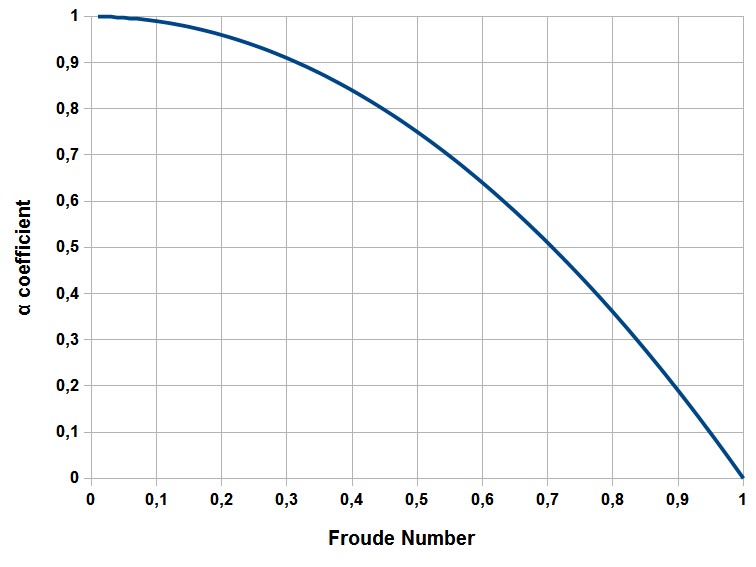
\includegraphics[width=0.8\textwidth]{Figures/Atten_Alpha.png}
  \caption{Coefficient $\alpha$ as a function of the Froude number}
 \end{center}
\end{figure}

With this simplification, the code \REZO{} is limited in its field of application: the subcritical flows.
This improves the robustness in various situations. In return, the fast phenomena are not represented. They are replaced by the calculation of a dummy water level that has no physical reality.
Therefore, the user must keep in mind the error committed by the code in rapid flow areas.


%----------------------------------------------------------------------------------------
%	CHAPTER 3: The F.V. Engines
%----------------------------------------------------------------------------------------
%-------------------------------------------------------------------------------
\chapter{The Finite Volumes unsteady transcritical engine \mascaret{}}
\label{Chapter3}
%-------------------------------------------------------------------------------

%-------------------------------------------------------------------------------
\section{Introduction}
%-------------------------------------------------------------------------------

The development of the transcritical engine originated from the need to have a code to carry out studies of flood waves, that also met the associated criteria of quality and performance.

The initial objective of the transcritical engine was, therefore, to allow the calculation of :
\begin{itemize}
 \item flow in valleys with bottom slopes possibly reaching 10\% over zones of limited size, and of strong variation of width (plunging gorges, rocky constrictions, etc...);
 \item very fast flows with the presence of discontinuities ;
 \item wave propagation over dry zones ;
 \item water lines in valleys several hundreds of km in length and with the presence of tributaries;
 \item water lines with supercritical reaches and the treatment of steady flow, for such applications as the flushing of reservoirs.
\end{itemize}

The various constraints listed above resulted, at a numeric level, in the adoption of a conservative scheme (the Roe scheme with biased treatment of the source terms) allowing for discontinuous solutions.

In the first part \ref{ESVTcons}, we recall the one-dimensional equations of Saint-Venant, written in a conservative form.

The second part is devoted to the numerical solution of the homogeneous problem and the source terms for a single reach. Presented in section \ref{resNumSVT} is the solution method used in the transcritical engine of \mascaret{}, with a \textit{finite volume} scheme explicit or implicit in time.

The explicit scheme can address highly unstationary problems such as flood waves. The numerical results are satisfactory but the constraint on the time step, due to the explicit scheme, is very restrictive for slightly unstationary flows and subcritical flows. This led to implicit the initial scheme linearly.

In the third part \ref{ModelCplx}, the more complex physical developments are presented such as the modelling of the compound channels, singularities (downstream dams, weirs, etc.) and confluences.

%-------------------------------------------------------------------------------
\section{Equations of Saint-Venant in a conservative form}
\label{ESVTcons}
%-------------------------------------------------------------------------------

%...............................................................................
\subsection{General form of the equations (a reminder)}
%...............................................................................

The flow in a river can generally be considered as one-dimensional, i.e. the function of only one variable of space, the curvilinear abscissa $x$ of the river channel.

The variables of the flow are therefore the discharge $Q$ and the wetted section $S$, functions of $x$ and of time $t$, and defined in each of the vertical sections of the river.

To obtain the equations of Saint-Venant starting from the equations of Navier-Stokes, it is supposed that the angle between the bottom and the horizontal is always small. Nevertheless, in practical application, we also need to compute zones with very strong slopes, but of limited extent.

In the hypothesis where the pressure within the fluid is hydrostatic and where the internal viscosity effects are negligible compared to the friction on the walls of the channel, $Q$ and $S$ are solutions of the equations of Saint-Venant and are written as \cite{GOUTAL91} \cite{AFIF86} :

\begin{equation}
 \label{SVT2}
 \left \lbrace
  \begin{array}{l}
    \frac{\partial S}{\partial t} + \frac{\partial Q}{\partial x} = q_a \\
    \\
    \frac{\partial Q}{\partial t} + \frac{\partial}{\partial x} \left ( \frac{\beta(x,S) Q^2}{S}\right ) + g S \frac{\partial Z}{\partial x} = g S J
  \end{array}
 \right.
\end{equation}
where:
\begin{itemize}
 \item $Z$ is the elevation of the free surface ($m$);
 \item $S$ is the wetted section ($m^2$);
 \item $g$ is the acceleration of gravity ($m.s^{-2}$);
 \item $J$ is the linear head loss from friction. $J$ is evaluated with the Strickler formula :
  \begin{equation}
    J = \frac{Q^2}{K^2 S^2 R_{h}^{4/3}}
  \end{equation}
  with $R_h$ the hydraulic radius and $K$ the Strickler friction coefficient.
\end{itemize}


It is reminded that the Strickler friction coefficient $K$ is equal to $1/n$ where $n$ is the Manning friction coefficient.

\begin{figure}[H]
 \begin{center}
  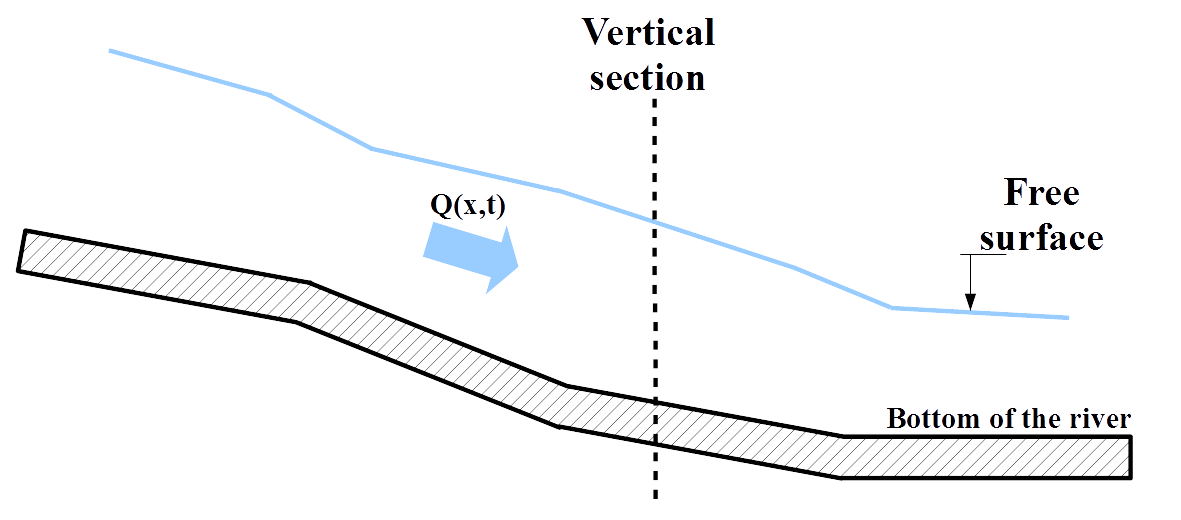
\includegraphics[width=\textwidth]{Figures/VueLong.png}
  \caption{Longitudinal view}
 \end{center}
\end{figure}

\begin{figure}[H]
 \begin{center}
  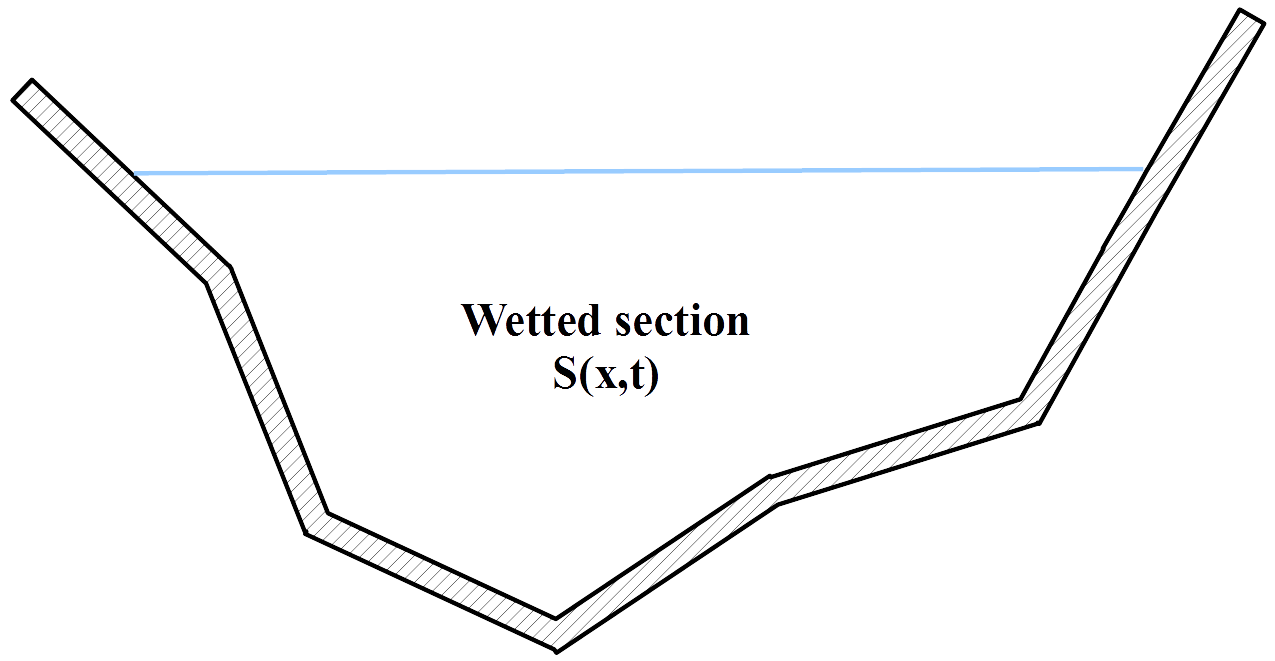
\includegraphics[width=\textwidth]{Figures/VueLat.png}
  \caption{Lateral view}
 \end{center}
\end{figure}

The dimensionless coefficient $\beta$, results from the variations of the actual velocity of the flow in a section :

\begin{equation}
 \beta(x,S) = \frac{S}{Q^2} \int V^2 \,dS
\end{equation}

In the case of a simple river channel, taking into account the hypothesis used to establish the equations of Saint-Venant, we take $\beta$ equal to 1, i.e. the variations of velocity within a section are neglected. This will not be true for a compound channel.


The system of equations (\ref{SVT2}) is obtained by expressing the conservation of mass for the first equation and the conservation of momentum for the second.

%...............................................................................
\subsection{Equations written in a conservative form}
%...............................................................................

A conservative system of equations can be expressed as :

\begin{equation}
  \frac{\partial W}{\partial t} + divF(W) = B(W)
\end{equation}
where:
\begin{itemize}
 \item $W$ is the vector of state;
 \item $F(W)$ is the flux;
 \item $B(W)$ is the source term.
\end{itemize}

Or, if there is only one dimension of space :

\begin{equation}
 \frac{\partial W}{\partial t} + \frac{\partial F}{\partial x} = B
\end{equation}

This way of writing the equation is interesting because it contains, in terms of distributions, the jump relationships in the case of a shock.

To write the conservative form of these equations from (\ref{SVT2}), we must transform the term : $g S \frac{\partial Z}{\partial x}$ in the dynamic equation. The first two terms of the dynamic equation : $\frac{\partial Q}{\partial t}$ and $\frac{\partial}{\partial x}\left ( \frac{Q^2}{S}\right )$ , correspond to the variation in momentum. This variation is equal to the action of external forces, i.e. the friction on the bottom represented by : $-g S J$ and the forces of gravity and pressure, which are taken into account by : $g S \frac{\partial Z}{\partial x}$.

The term $g S \frac{\partial Z}{\partial x}$ can be transformed by using the term for pressure : $P = g \int_{0}^{y} S \, dy$, where : $y = Z - Z_f$, $Z$ being the free surface elevation and $Z_f$ the bottom elevation.

\begin{figure}[H]
 \begin{center}
  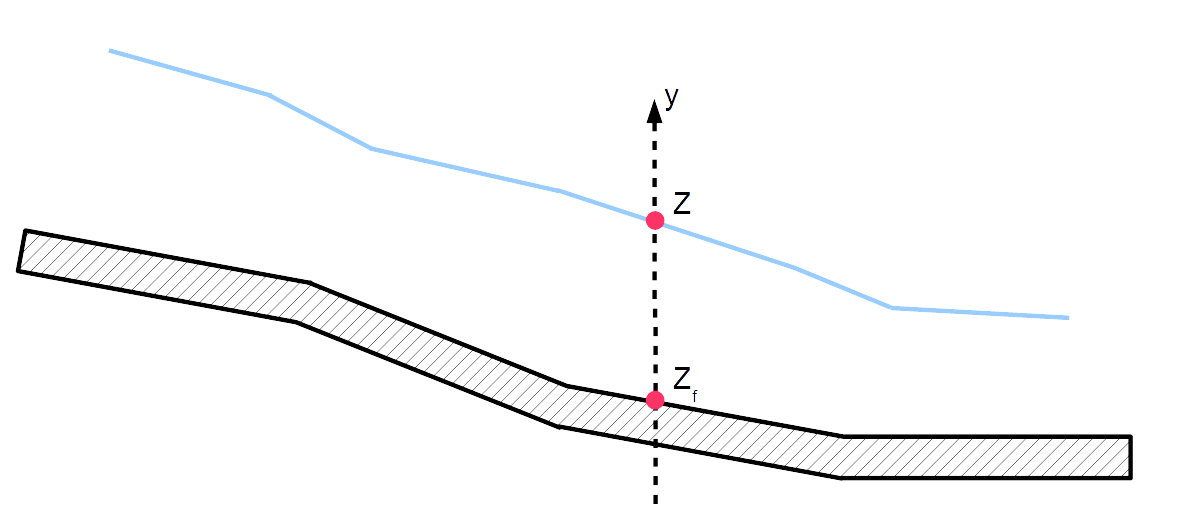
\includegraphics[width=\textwidth]{Figures/VueLong2.png}
  \caption{Longitudinal view : the elevations}
 \end{center}
\end{figure}

We can write :

\begin{equation}
 \frac{\partial P}{\partial x} = g S \frac{\partial y}{\partial x} + g \int_{0}^y \left ( \frac{\partial S}{\partial x}\right ) \, dy
\end{equation}

which is equivalent to :

\begin{equation}
 \frac{\partial P}{\partial x} = g S \frac{\partial Z}{\partial x} + g \int_{0}^y \left ( \frac{\partial S}{\partial x}\right ) \, dy - g S \frac{\partial Z_f}{\partial x}
\end{equation}

The dynamic equation can be re-written as :

\begin{equation}
 \frac{\partial Q}{\partial t} + \frac{\partial}{\partial x} \left ( \frac{Q^2}{S} + P \right ) = g \int_{0}^y \left ( \frac{\partial S}{\partial x} \right )_y \, dy - g S \frac{dZ_f}{dx} - g S J
\end{equation}

It is noted that the source term related to the geometry of the dynamic equation can equally be written : $\left( \frac{\partial P}{\partial x} \right )_{z = constant}$.

The source term of this new equation depends only on the variables $Q$ and $S$ of the geometry of the river, it does not depend on the derivative in respect to $x$ or $t$ of $Q$ and $S$. In effect, the derivative : $\left ( \frac{\partial S}{\partial x} \right )_y$ is purely geometrical (here $S$ indicates the geometric section and not the wetted section). This equation is written in a conservative form.

So, the conservative formulation of the equations of the system (\ref{SVT2}) is (with : $q_a = 0$) :

\begin{equation}
 \label{SVT3}
 \left \lbrace
  \begin{array}{l}
    \frac{\partial S}{\partial t} + \frac{\partial Q}{\partial x} = 0 \\
    \\
    \frac{\partial Q}{\partial t} + \frac{\partial}{\partial x} \left ( \frac{Q^2}{S} + P \right ) = g \int_{0}^y \left ( \frac{\partial S}{\partial x} \right )_y \, dy - g S \frac{dZ_f}{dx} - g S J
  \end{array}
 \right.
\end{equation}

with : $P = g \int_{0}^{y} S \, dy$

This equation is actually of the form :

\begin{equation}
 \frac{\partial W}{\partial t} + \frac{\partial F}{\partial x} = B
\end{equation}

with :

\begin{equation}
 W = \left ( \frac{S}{Q} \right )
\end{equation}

\begin{equation}
 F = \left (
    \begin{array}{c}
    Q \\
    \\
    \frac{Q^2}{S} + P
\end{array}
\right )
\end{equation}
and :
\begin{equation}
 B = \left (
    \begin{array}{c}
    0 \\
    \\
    g \int_{0}^y \left ( \frac{S}{x} \right )_y \, dy - g S \frac{dZ_f}{dx} - g S J
\end{array}
\right )
\end{equation}

\begin{CommentBlock}{Comment :}
\begin{itemize}
 \item The flux depends not only on $W$ but also on $x$. Knowing only $W$ is not sufficient to calculate $F$. In effect, the term for pressure $P$ appearing in $F$ can only be evaluated if the wetted section and the variation of the section based on the flow depth are known explicitely. However the variation of the section depends on the geometry of the river. Therefore it can only be know if the $x$ axis is given. We will see the importance of this statement in the search for the Riemann invariants of the system of equations (\ref{SVT3});
 \item The variables $Q$ and $S$ can be discontinuous (e.g. in the case of a hydraulic jump). The derivatives appearing in (\ref{SVT3}) therefore need to be understood in the sense of distributions. Actually, in this case, the system (\ref{SVT3}) is the only correct equation system, because in (\ref{SVT2}) the term : $g S \frac{\partial Z}{\partial x}$ has no meaning, both in a classical sense and in the sense of the distributions.
\end{itemize}
\end{CommentBlock}

%...............................................................................
\subsection{Riemann invariants}
%...............................................................................

The system (\ref{SVT3}) is hyperbolic. The jacobian matrix of $F$ : $\left ( \frac{\partial F}{\partial W} \right )_x$  admits two real and distinct eigenvalues : $\lambda^+$ et $\lambda^-$ :

\begin{equation}
 \left ( \frac{\partial F}{\partial W} \right )_x = \left (
    \begin{array}{c c}
    0 & 1\\
    \\
    -\frac{Q^2}{S^2} + \left ( \frac{\partial P}{\partial S} \right )_x & \frac{2 Q}{S}
\end{array}
\right )
\end{equation}

\begin{equation}
 \left \lbrace
  \begin{array}{l}
    \lambda^+ = \frac{Q}{S} + C \\
    \\
    \lambda^- = \frac{Q}{S} - C \\
  \end{array}
 \right.
\end{equation}

with :

\begin{equation}
 C = \sqrt{\left ( \frac{\partial P}{\partial S} \right )_x}
\end{equation}

The celerity $C$ is only a function of $S$ and $x$.

In using the properties of the hyperbolic systems \cite{GODLEWSKI91}\cite{AFIF86}, (\ref{SVT3}) can be rewritten in the form of two convection equations of the Reiman invariants.

We do not give the details of the calculations here (see \cite{GODLEWSKI91} and \cite{AFIF86}).

We finally obtain the system (\ref{SVT4}) :

\begin{equation}
 \label{SVT4}
 \left \lbrace
  \begin{array}{l}
    \frac{df^-}{dt} = - \lambda^- \int_{0}^S \frac{1}{S} \left ( \frac{\partial C}{\partial x}\right )_S dS - g \left ( \left ( \frac{\partial y}{\partial x} \right )_S + \frac{dZ_f}{dx} + J \right ) \\
    \\
    \frac{df^+}{dt} = + \lambda^+ \int_{0}^S \frac{1}{S} \left ( \frac{\partial C}{\partial x}\right )_S dS - g \left ( \left ( \frac{\partial y}{\partial x} \right )_S + \frac{dZ_f}{dx} + J \right )
  \end{array}
 \right.
\end{equation}

where :
\begin{itemize}
 \item $\frac{df^-}{dt} = \frac{\partial f^-}{\partial t} + \lambda^- \frac{\partial f^-}{\partial x}$ is the derivative of the Reimann invariant : $f^- = \frac{Q}{S} - K$ with $K = \int_{0}^S \frac{C}{S} \, dS$ along the characteristic curve $C^-$ of slope : $\frac{dx}{dt} = \lambda^-$;
 \item $\frac{df^+}{dt} = \frac{\partial f^+}{\partial t} + \lambda^+ \frac{\partial f^+}{\partial x}$ is the derivative of the Reimann invariant : $f^+ = \frac{Q}{S} + K$ along the characteristic curve $C^+$ of slope : $\frac{dx}{dt} = \lambda^+$.
\end{itemize}

We refer to the subcritical characteristic as the curve $C^+$, and to the supercritical characteristic as the curve $C^-$.

Expressing (\ref{SVT3}) in the form of equations along the characteristic curves is equivalent to considering two mobile markers moving along the characteristics. The discharge and the wetted section at a point in the channel at a given time, are determined by the information provided by the characteristics $C^+$ and $C^-$ which intersect at this point.

\begin{figure}[H]
 \begin{center}
  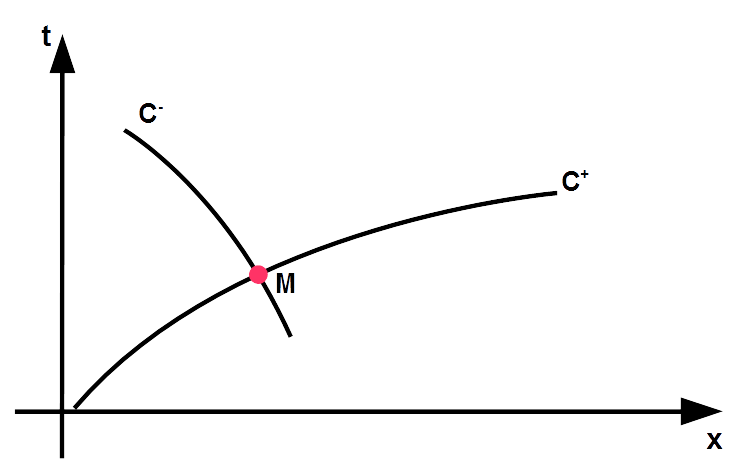
\includegraphics[width=0.8\textwidth]{Figures/2Carac.png}
  \caption{The two characteristic curves}
 \end{center}
\end{figure}

Knowing $f^+$ and $f^-$ (calculated with the help of the information conveyed by the characteristics in $M$), we can deduce $Q$ and $S$.

Formulating the system (\ref{SVT3}) in the form of characteristics also allows it to remain \textit{related} to the physical problem during the computational process. We will see an interesting application of this during the processing of the boundary conditions (see section \ref{PriseCL}).

However, the system (\ref{SVT4}) is only equivalent to the system (\ref{SVT3}) when the flow has no discontinuities. The development of the derivative $\frac{\partial F}{\partial x}$ used to obtain the system (\ref{SVT4}) is not possible in the presence of a discontinuity.

%...............................................................................
\subsection{The hydraulic jump}
%...............................................................................

\begin{CommentBlock}{Note :}
we use the terms \textit{hydraulic jump} and \textit{shock} indifferently when describing a discontinuity.
\end{CommentBlock}

A shock appears in a flow when two characteristics of the same family intersect. Two types of shock exist :
\begin{itemize}
 \item the one due to the intersection of characteristics $C^-$ : shock $C^-$;
 \item the other due to the meeting of characteristics $C^+$ : shock $C^+$.
\end{itemize}

At the point where the characteristics meet, two values of $f^-$ (for a $C^-$ shock) or two values of $f^+$ (for a $C^+$ shock) are introduced, in addition to the information derived from the other family of characteristics. This overload of information, mathematically unacceptable, results in a discontinuity at the intersection. From a physical point of view it results in the establishment of a dissipative process : the hydraulic jump.

\begin{figure}[H]
 \begin{center}
  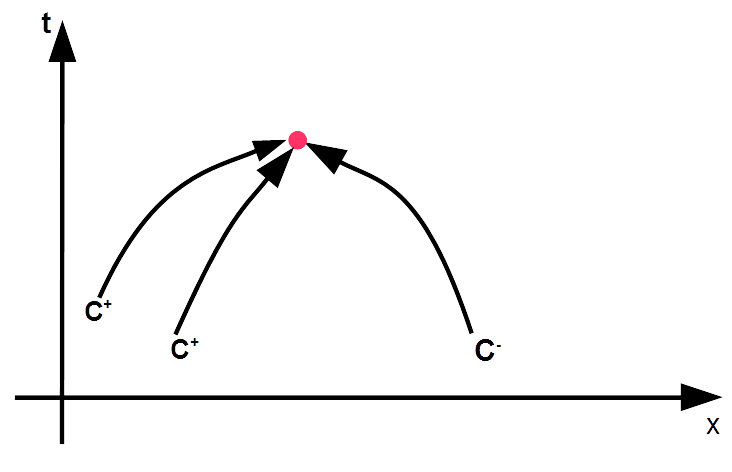
\includegraphics[width=\textwidth]{Figures/3Carac.png}
  \caption{Example of a $C^+$ shock}
 \end{center}
\end{figure}

The trajectory of the shock is made of all the points where characteristics of the same family intersect.

\begin{figure}[H]
 \begin{center}
  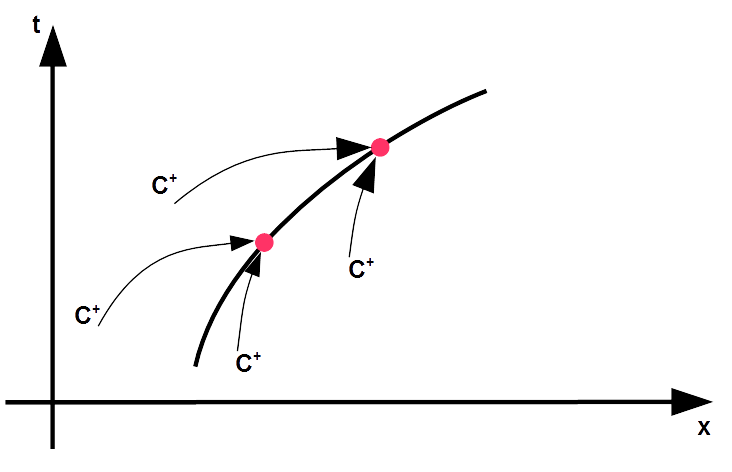
\includegraphics[width=\textwidth]{Figures/Trajec_Choc.png}
  \caption{Trajectory of a $C^+$ shock}
 \end{center}
\end{figure}

To the left and to the right of the shock, the matrix $\left ( \frac{\partial F}{\partial W} \right )_x$ is well defined, it is similarly true for its eigenvalues which are $(\lambda_{g}^+,\lambda_{g}^-)$ to the left and $(\lambda_{d}^+,\lambda_{d}^-)$ to the right.

The speed $s^-$ of a $C^-$ shock verifies :
\begin{equation}
  \left \lbrace
  \begin{array}{l}
    \lambda_{d}^- < s^- < \lambda_{g}^- (< \lambda_{g}^+) \\
    s^- < \lambda_{d}^+
  \end{array}
 \right.
\end{equation}

and the speed $s^+$ of a $C^+$ shock verifies :
\begin{equation}
  \left \lbrace
  \begin{array}{l}
    (\lambda_{d}^- < ) \lambda_{d}^+ < s^+ < \lambda_{g}^+  \\
    \lambda_{g}^- < s^+
  \end{array}
 \right.
\end{equation}

Indeed, the characteristics that create the shock catch this shock up from upstream (here to the left) and are caught up by it on the downstream (here on the right). This is the meaning of the first inequalities for the $C^-$ shocks and the $C^+$ shocks : the speed of the shock is intermediate between those of the characteristics that create it. The meaning of the second inequalities is that there cannot be a $C^-$ and a $C^+$ at the same point : the velocity of a shock cannot be between the velocities of characteristics that did not take part in its creation.

Therefore, the scheme shown in figure \ref{fig:Timp} will never be found.

\begin{figure}[H]
 \begin{center}
  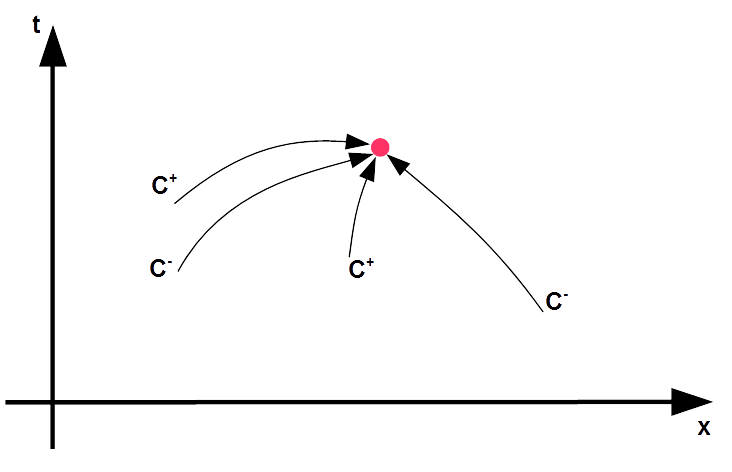
\includegraphics[width=\textwidth]{Figures/Trajec_imposs.png}
  \caption{Example of a characteristics scheme that is not possible}
  \label{fig:Timp}
 \end{center}
\end{figure}

These inequalities are all the information that the characteristics provide about the shock. Originating from a non-conservative formulation of the equations, they do not lead to a quantitative description of shocks. The states to the left and the right of a shock can not be determined by the Riemann invariants provided by the characteristics intersecting at the shock. However, for weak shocks, the speed of a shock is the average of the speed $\lambda_g$ and $\lambda_d$ of the characteristics that create it \cite{SMOLLER83}\cite{LAX72}).

The only way to describe shocks correctly is to come back to the equations written in a conservative form. When the flow contains a hydraulic jump, the homogeneous hyperbolic system, interpreted in the sense of distributions, allows to connect the states to the left and right of the hydraulic jump \cite{GODLEWSKI91}.

The relations thereby obtained are the jump conditions (these are also sometimes called Rankine-Hugoniot conditions). They are written as, with $s$ is the celerity of the hydraulic jump :

\begin{equation}
   \left \lbrace
  \begin{array}{l}
   s ( S_d -S_g ) = Q_d - Q_g \\
   s ( Q_d - Q_g ) = \left ( \frac{Q_{d}^2}{S_d} + P_d \right ) - \left ( \frac{Q_{g}^2}{S_g} + P_g \right )
  \end{array}
 \right.
\end{equation}

\begin{figure}[H]
 \begin{center}
  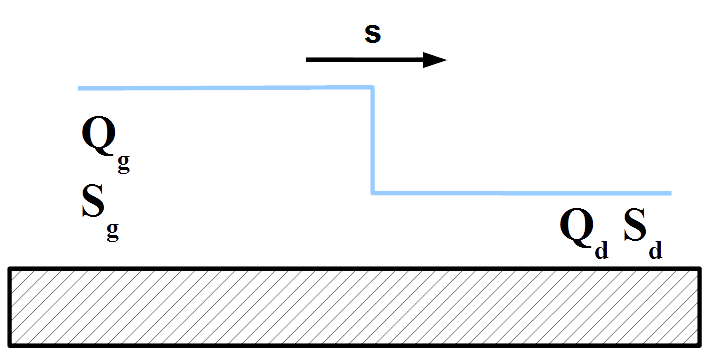
\includegraphics[width=\textwidth]{Figures/vitesse.png}
  \caption{Celerity of the hydraulic jump}
 \end{center}
\end{figure}

\begin{CommentBlock}{Comments :}
\begin{itemize}
 \item The Rankine-Hugoniot conditions are only a particular form of the system of equations (\ref{SVT3}). This can be demonstrated by doing a balance of the mass and the momentum over a slice of fluid including the hydraulic jump. In the equation of momentum, the source term disappears when the width of the slice tends towards zero.
 \item In the coordinate system of the hydraulic jump (in translation at speed $s$), the discontinuity always separates a supercritical flow from a subcritical flow. \\ In the frame of reference of the hydraulic jump : $s = 0$, so : $Qd = Qg = Qrel$ relative discharge.\\
The function :$f(S,x) = \frac{Q_{rel}^2}{S} + P$ has the same value on both sides of the jump.\\
Moreover $f$ admits a minimum for $S$ such that : $\left ( \frac{\partial f}{\partial S}\right )_x = 0$, i.e. : $Q_{rel} = C S$. The value of : $S = \frac{Q_{rel}}{C}$ corresponds to a critical flow (Froude number equal to 1). Two values of $S$ giving the same value of f (Rankine-Hugoniot condition) are therefore located on each side of the critical section.
\end{itemize}
\end{CommentBlock}

%-------------------------------------------------------------------------------
\section{Numerical solution of the St-Venant equations}
\label{resNumSVT}
%-------------------------------------------------------------------------------

%...............................................................................
\subsection{The explicit scheme}
\label{SchemExp}
%...............................................................................

In this section, we describe the numerical methods used in \mascaret{} to solve the system of equations (\ref{SVT3}). A explicit scheme was developed first, then the transcritical engine was made implicit. This leaves the choice of using one of the two schemes to the user.

%...............................................................................
\subsubsection{Description of the problem}
%...............................................................................

The system to solve is as follows :

\begin{equation}
   \label{sys}
   \left \lbrace
  \begin{array}{l}
   W = (S,Q) \\
   \\
   \frac{\partial W}{\partial t} + \frac{\partial F(W,x)}{\partial x} = B(x,W) \qquad (x,t) \in [a,b] \times [0,T]
  \end{array}
 \right.
\end{equation}

with :

\begin{equation}
 F(x,W) = \left ( \begin{array}{c}
    Q\\
    \\
    \frac{Q^2}{S} + P(x,S)
\end{array}
\right )
\end{equation}

and :

\begin{equation}
 B(x,W) = \left ( \begin{array}{c}
    0\\
    \\
    g \int_{0}^y \left ( \frac{\partial S}{\partial x} \right )_y \, dy - g S \frac{dZ_f}{dx} - g S J
\end{array}
\right )
\end{equation}

So that this problem is well presented, it is necessary to add an initial condition and boundary conditions.

The problem (\ref{sys}) to be solved, is a strictly hyperbolic system where the source term is dominant in the calculation of the flow (see the previous section).
Considering that the scope of application of the \mascaret{} code is primarily the calculation of flood waves, this implies :
\begin{itemize}
 \item geometry with very steep slopes (locally reaching $10\%$ possibly) and large variations of width;
 \item very fast flows (speeds above $10 m/s$);
 \item wave propagation over dry areas;
 \item very long computational domains.
\end{itemize}

In addition to the flood wave calculations, the intention is to be able to model any flow presenting a supercritical regime such as the flushing of reservoirs and the steady flows in torrents. This adds an additional constraint, which is that the source term must be correctly calculated in order to obtain a correct convergence towards steady flows. The objective was to find a scheme that complies with these various constraints (which can sometimes be contradictory) as closely as possible.
\vspace{0.5cm}

For now we are interested only in the numerical solution of the homogeneous problem. A following section, \ref{TrtSource} is devoted to the treatment of the source terms.

%...............................................................................
\subsubsection{Solution of the homogeneous problem}
\label{PbHom}
%...............................................................................

The homogeneous problem to solve is written :

\begin{equation}
 \frac{\partial W(x,t)}{\partial t} + \frac{\partial F(W)}{\partial t} = 0
\end{equation}

This homogeneous problem is very similar to the isentropic Euler equations. The principle difference resides in the fact that the flux does not depend solely on the state variables (which are the wetted section and the discharge) but also depends on the variable of space $x$. Moreover, the pressure term is not known explicitely but is a tabulated variable.

The time interval $[0,T]$ is discretised in a series of intervals $[t_n , t_{n+1}]$ with : $t_{n+1} = t_n + \Delta t$ where $\Delta t$ is the time step.

The computational domain will be discretised in $N$ intervals $[x_i , x_{i+1}]$ with : $\Delta x_i = x_{i+1} - x_i$.

We denote $x_{i+1/2}$ the midpoint of the interval $[x_i , x_{i+1}]$.

The scheme used is a finite volume scheme based on a integral formulation of the mass and momentum balance over a cell $[x_{i-1/2},x_{i+1/2}]$ (see figure \ref{fig:Schm1}).

\begin{figure}[H]
 \begin{center}
  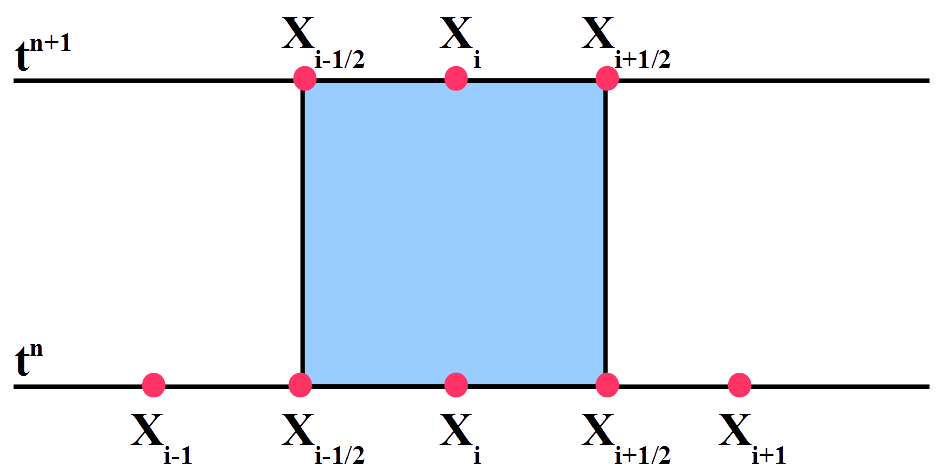
\includegraphics[width=\textwidth]{Figures/Schema1.png}
  \caption{Finite volume cell}
  \label{fig:Schm1}
 \end{center}
\end{figure}

\begin{CommentBlock}{Note :}
$\underline{W}_h = \left \lbrace \Psi_h \in L^2 (\Omega), \Psi_{h/]x_{i-1/2},x_{i+1/2}[} = constant, i = 1..N \right \rbrace$
\end{CommentBlock}

A variational description of the problem (\ref{sys}) can be formulated as :

find $W_h(S_h,Q_h) \in \underline{W}_h$ such as :

\begin{equation}
 \label{fvar}
 \int_{t_n}^{t_{n+1}} \int_{a}^{b} \left ( \frac{\partial W_h}{\partial t} + \frac{\partial F(x,W_h)}{\partial x} \right ) \Psi_h \, dx \, dt = 0 \qquad \forall \Psi_h \in \underline{W}_h
\end{equation}

Each function $\Psi_h$ of $\underline{W}_h$ is determined in a unique way by :

\begin{equation}
 \Psi_h = \sum_{i=1}^n \Psi (a_i)\phi_i
\end{equation}
with $\left \lbrace \varphi_i\right \rbrace_{i=1,N}$ which forms a base of $\underline{W}_h$. In fact, the functions of base $\varphi_i$ are the characteristic functions of the interval $[x_{i-1/2},x_{i+1/2}]$.

By writing the variational equation (\ref{fvar}) for each base function and by using the Green formula, we obtain :

\begin{eqnarray}
 & \int_{x_{i-1/2}}^{x_{i+1/2}} W_{h}^{n+1}\, dx = \int_{x_{i-1/2}}^{x_{i+1/2}} W_{h}^{n}\, dx + \int_{t^n}^{t^{n+1}} F(x_{i+1/2},W_{i+1/2}) \, dt  &         \nonumber \\
 & - \int_{t^n}^{t^{n+1}} F(x_{i-1/2},W_{i-1/2}) \, dt &
\end{eqnarray}

$W_{h}^{n+1}$ being sought in the space of the functions that are constant per cell, the previous equation becomes :

\begin{eqnarray}
 & W_{i}^{n+1} = W_{i}^n + \frac{1}{x_{i+1/2}-x_{i-1/2}} & \nonumber \\
 & \times \left ( \int_{t^n}^{t^{n+1}} F(x_{i+1/2},W_{i+1/2}) \, dt - \int_{t^n}^{t^{n+1}} F(x_{i-1/2},W_{i-1/2}) \, dt \right ) &
\end{eqnarray}

The problem can therefore be reduced to the evaluation of the numerical flux at each interface. Moreover, $W_{n+1}$ being a function constant per cell, the calculation of the numerical flux will require the solution of a Riemann problem at each interface.

Therefore, at each time step and each cell interface, the following problem needs to be solved :

\begin{equation}
 \label{sysW}
 \left \lbrace
  \begin{array}{l}
   \frac{\partial W_h}{\partial t} + \frac{\partial F(x_{i+1/2},W_h)}{\partial x} = 0 \\
   \\
   W_{h}^n = \left \lbrace
             \begin{array}{l}
               W_{i}^n \qquad \mbox{si} \quad x < x_{i+1/2} \\
               W_{i+1}^n \qquad \mbox{si} \quad x > x_{i+1/2}
             \end{array}
             \right.
  \end{array}
 \right.
\end{equation}

To solve this problem, it is natural to consider a Godunov scheme, based on the exact solving of the Riemann problem at each interface. However, the interest of this exact solution is counterbalanced by the fact that firstly the projection on each cell can cause a loss of quality from the exact solving, and secondly an exact Rieman solver is computationally expensive. For this reason an approximate Riemann solver has been chosen. More specifically, we have retained the Roe scheme which will be presented in the following paragraph. Moreover, another reason to choose the Roe scheme is that it is widely used for solving Euler and Saint-Venant equations \cite{PAQUIER95}\cite{VAZQUEZ94}\cite{AMBROSI95}\cite{MONTHE97}.

%...............................................................................
\subsubsection{Roe linearisation}
\label{LinRoe}
%...............................................................................

The aim here is to define a Riemann problem \textit{close} to (\ref{sysW}) but for which the solution is simpler to calculate. To do this, we apply the Roe linearisation method. This method is well known and widely used. We recall the main references where the reader can find the details of the calculation of the Roe linearisation \cite{ROE81}\cite{BUFFARD93}.

The principle of the Roe linearisation method rely on the fact that there exists a matrix A (called 'Roe linearised') verifying :
\begin{itemize}
 \item[*] $F(W_g) - F(W_d) = A(W_g,W_d)(W_g-W_d)$;
 \item[*] $A(W,W) = DF_{w}(W)$;
 \item[*] the matrix $A(W,W)$ has real eigenvalues and the eigenvectors generate the complete space.
\end{itemize}

\begin{CommentBlock}{Comment: }
The Roe linearisation method defined here is only valid for cases were the flux F depends solely on the state variables. Nevertheless, this method has been applied in the present case.
\end{CommentBlock}

The Roe scheme cannot be used if it is not possible to find a matrix satisfying these three properties. In this context, the difficulty lies with the fact that the flux depends on $x$ and the state variables.

To calculate the Roe matrix, the method is similar to that used for the isentropic Euler equations i.e. an average state is sought, so that the Roe matrix is the jacobian matrix of the flux taken in that average state.

In our case, the average of Roe $\tilde W$ is given by :
\begin{equation}
 \tilde W = \frac{W_g \sqrt{S_g} + W_d \sqrt{S_d}}{\sqrt{S_g} + \sqrt{S_d}}
\end{equation}
where :
\begin{itemize}
 \item $W_g \left ( \begin{array}{c}
    S_g\\
    V_g
    \end{array} \right )$ indicates the state to the left;
 \item and $W_d \left ( \begin{array}{c}
    S_d\\
    V_d
    \end{array} \right )$ the state to the right;
\end{itemize}

The Roe matrix $\tilde A (x,W_g,W_d)$ is the jacobian $A(x,W)$ calculated in this state.

\begin{equation}
 A(x,\tilde W) = \left ( \begin{array}{cc}
       0 & 1 \\
       \frac{-\tilde{Q}^2}{\tilde{S}^2} + \frac{\partial P(x,\tilde S )}{\partial S} & 2 \frac{\tilde Q}{\tilde S}
    \end{array} \right ) \quad \mbox{with } \tilde W (\tilde S , \tilde Q)
\end{equation}

The Riemann problem is therefore equivalent to the following linearised problem at each interface :

\begin{equation}
 \label{sysW2}
 \left \lbrace
  \begin{array}{l}
   \frac{\partial W(x,t)}{\partial t} + \tilde A(x_{i+1/2},W_g,W_d) \frac{\partial W(x,t)}{\partial x} = 0 \\
   \\
   W(x,t^n) = \left \lbrace
             \begin{array}{l}
               W_{g} \quad \mbox{si : } x < x_{i+1/2} \\
               W_{d} \quad \mbox{si : } x > x_{i+1/2}
             \end{array}
             \right.
  \end{array}
 \right.
\end{equation}

with : $\tilde A(x_{i+1/2},W_g,W_d) = A(x_{i+1/2},\tilde W)$

The solution of the linear problem (\ref{sysW2}) will allow the Roe scheme to be fully explicited.

\begin{CommentBlock}{Comment :}
The Roe matrix is evaluated at the interface $x_{i+1/2}$.
\end{CommentBlock}

%...............................................................................
\subsubsection{The Roe solver}
%...............................................................................

The solution of the problem (\ref{sysW2}) is simple. It consists of 3 constant states separated by jumps through the characteristics defined by :

\begin{equation}
  \frac{x}{t}=\lambda_{1,2}
\end{equation}

with :

\begin{equation}
 \lambda_1(x,S,Q) = \frac{Q}{S} - C(x,S)
\end{equation}

\begin{equation}
 \lambda_2(x,S,Q) = \frac{Q}{S} + C(x,S)
\end{equation}

and :

\begin{equation}
 C(x,S) = \frac{\partial P(x,S)}{\partial S}
\end{equation}

We can note that :
\begin{equation}
 \left \lbrace
  \begin{array}{l}
   W_g = \sum_{i=1,2} \alpha_{ig}(W_g,W_d) r_i(W_g,W_d) \\
   W_d = \sum_{i=1,2} \alpha_{id}(W_g,W_d) r_i(W_g,W_d)
\end{array}
 \right.
\end{equation}
where $r_i$ are the right side eigenvectors associated with the eigenvalue $\lambda_i$.

By supposing $\lambda_1 < \lambda_2$, the solution is written:
\begin{equation}
 W(\frac{x}{t},W_g , W_d ) = \left \lbrace
  \begin{array}{l}
   W_g \quad \mbox{if : } \frac{x}{t} < \lambda_1 (x,W_g,W_d) \\
   W_m \quad \mbox{if : } \lambda_1 < \frac{x}{t} < \lambda_2 \\
   W_d \quad \mbox{if : } \frac{x}{t} > \lambda_2 (x,W_g,W_d)
  \end{array}
 \right.
\end{equation}
with : $W_m = \alpha_{1d} r_1 (W_d,W_g) + \alpha_{2g} r_2 (W_d,W_g)$

$A$ is the jacobian matrix of $F$ which is diagonalisable in the basis of the eigenvectors $X$. $A$ is therefore equal to : $X \Lambda X^{-1}$

$|\Lambda|$ is the diagonal matrix of the generic term $|\Lambda_i|$, $\Lambda^{+}$ and $\Lambda^{-}$ defined respectively by :
\begin{equation}
  \left \lbrace
  \begin{array}{l}
   \Lambda_{i,j}^{+}  = \lambda_{i}^{+} \delta_{i,j}\\
   \Lambda_{i,j}^{-}  = \lambda_{i}^{-} \delta_{i,j}
\end{array}
 \right.
\end{equation}

In the same way $A^+$, $A^-$ et $|A|$ are defined by :
\begin{equation}
  \left \lbrace
  \begin{array}{l}
   A^{+}  = X \Lambda^{+} X^{-1} \\
   A^{-}  = X \lambda^{-} X^{-1} \\
   |A| = X |\lambda| X^{-1}
\end{array}
 \right.
\end{equation}

The Roe flux therefore takes the following form :

\begin{eqnarray}
 F(x_{i+1/2},W_g,W_d) & = & \frac{1}{2} \left ( F(x_{i+1/2},W_g) + F(x_{i+1/2},W_d) \right ) \nonumber \\
                      &   & + \frac{1}{2} \left | \tilde{A}(x_{i+1/2},W_g,W_d) \right | (W_d -W_g) \nonumber \\
 & = & F(x_{i+1/2},W_d) - \tilde{A}^+ (x_{i+1/2},W_d,W_g) (W_d - W_g) \nonumber \\
 & = & F(x_{i+1/2},W_g) + \tilde{A}^- (x_{i+1/2},W_d,W_g) (W_d - W_g) \nonumber \\
 & &
\end{eqnarray}

From the definition of the flux, the scheme is completely defined. This scheme is first-order in space and time.  Moreover, this scheme is stable if the Courant number is less than 1.

%...............................................................................
\subsubsection{Entropic correction}
%...............................................................................

The main drawback of the Roe scheme is that it is not entropic and can therefore admit non-entropic stationary discontinuities in the vicinity of the sonic points, i.e. where an eigenvalue associated with a nonlinear field of jacobian matrix changes sign on both sides of an interface. To avoid this problem, it is therefore necessary to modify the calculation of the flux in the vicinity of the points were an eigenvalue $\lambda_{m=1,2} (\tilde W )$ is close to zero.

It is possible to consider several modifications of the eigenvalue $\lambda_{m} (\tilde W )$ We have retained the entropic correction defined by Leveque \cite{LEVEQUE90}. $\lambda_{m} (\tilde W )$ is replaced by : $\lambda_m (W_d) \left ( \frac{\lambda_m (\tilde W) - \lambda_m (W_g)}{\lambda_m (W_d) - \lambda_m (W_g)}\right )$

\begin{CommentBlock}{Comment :}
A second-order on time scheme would remove the need for the entropic correction.
\end{CommentBlock}

%...............................................................................
\subsection{Use of the implicit scheme}
%...............................................................................

%...............................................................................
\subsubsection{Introduction}
%...............................................................................

This paragraph describes the implicit scheme developed in the \mascaret{} code. The aim of this development was to lift the time step constraint coming from the CFL condition for an explicit scheme (see section  \ref{SchemExp}). The applications targeted by this development are essentially subcritical situations (propagation of medium floods) for which the numerical constraint on the time step is very detrimental in terms of computing time.

This scheme is based on a linear implicitation of the Roe-type finite-volumes scheme. The linear scheme is solved by a direct method that avoids the convergence problems of an iterative method when the matrix is poorly conditioned. The direct method is a method of decomposition of type $LU$ adapted to tri-diagonal block matrices.

The results obtained with the implicit scheme on validation cases are detailed in the note \cite{GOUTAL02}. The study cases include both analytical tests and more complex tests representative of real applications : propagation of floods, flushing of reservoirs and flood waves.

%...............................................................................
\subsubsection{Reminder and interest of the implicitation}
%...............................................................................

We recall that the problem to solve, detailed in section \ref{ESVTcons} (the St-Venant equations written in their conservative form), is a strictly hyperbolic system with a prominent source term :

\begin{equation}
  \label{PbP}
   \left \lbrace
  \begin{array}{l}
   W = (S,Q) \\
  \\
   \frac{\partial W}{\partial t} + \frac{\partial F(W,x)}{\partial x} = B(x,W) \quad (x,t) \in [a,b] \times [0,T]
\end{array}
 \right.
\end{equation}

with :
\begin{equation}
 F(W,x) = \left ( \begin{array}{c}
       Q \\
       \frac{Q^2}{S} + P(x,S)
    \end{array} \right )
\end{equation}

and :
\begin{equation}
 B(x,W) = \left ( \begin{array}{c}
       0 \\
       g \int_{0}^y \left ( \frac{\partial S}{\partial x} \right )_y \, dy - g S \frac{\partial Z_f}{\partial x} - g S J
    \end{array} \right )
\end{equation}

The numerical scheme used to solve this problem is detailed in the previous section : the scheme used is a finite volume scheme based on the integral formulation of the balance of mass and of momentum on a cell, $[x_{i-1/2}, x_{i+1/2}]$ (see section \ref{PbHom}).

After a discretisation of the scheme in time and space, and if the discrete solution is sought in the space of the functions constant over a cell, the problem (\ref{PbP}) is written :

\begin{eqnarray}
  W_{i}^{n+1} & = & W_{i}^{n} - \frac{1}{x_{i+1/2}-x_{i-1/2}} \nonumber \\
              &   & \times \left ( \int_{t^n}^{t^{n+1}} F(x_{i+1/2},W_{i+1/2})\, dt - \int_{t^n}^{t^{n+1}} F(x_{i-1/2},W_{i-1/2})\, dt  \right ) \nonumber \\
              &   & + B_{i+1/2}^n - B_{i-1/2}^n
\end{eqnarray}

with :
\begin{itemize}
  \item $\Delta t$ the time step and : $t_{n+1} = t_n + \Delta t$;
  \item $\Delta x = x_{i+1} - x_{i}$;
  \item $x_{i+1/2}$ the midpoint of the interval $[x_i , x_{i+1}]$.
\end{itemize}

The problem is then reduced to the evaluation of the numerical flux F at each interface ; as done for the Roe scheme (see \ref{LinRoe}) and recalled below. The source terms are evaluated with a mixed treatment, centered and decentered, which is detailed in the following section.

The jacobian matrix $A$ of the function $F$ is diagonalisable in the basis of the eigenvectors $X$. $A$ is therefore equal to $X \Lambda X^{-1}$.

$\tilde A$ denote the Roe Matrix : $\tilde A = \tilde X \tilde \Lambda \tilde{X}^{-1}$

$|\Lambda|$ is the matrix of generic term $|\Lambda_i|$, $\Lambda^+$ and $\Lambda^-$ are respectively defined by : $\Lambda_{i,j}^+ = \lambda_{i}^+ \delta_{i,j}$ and $\Lambda_{i,j}^- = \lambda_{i}^- \delta_{i,j}$.

In the same way $\tilde{A}^+$, $\tilde{A}^-$ and $|\tilde A|$ are defined by : $\tilde{A}^+ = \tilde X \tilde{\Lambda}^+ \tilde{X}^{-1}$, $\tilde{A}^- = \tilde X \tilde{\Lambda}^- \tilde{X}^{-1}$ and $|\tilde A| = \tilde X |\tilde \Lambda| \tilde{X}^{-1}$.

Therefore, the Roe flux takes the following form :

\begin{eqnarray}
 F(x_{i+1/2},W_g,W_d) & = & \frac{1}{2} \left ( F(x_{i+1/2},W_g) + F(x_{i+1/2},W_d) \right ) \nonumber \\
                      &   & + \frac{1}{2} \left | \tilde{A}(x_{i+1/2},W_g,W_d) \right | (W_d -W_g) \nonumber \\
 & = & F(x_{i+1/2},W_d) - \tilde{A}^+ (x_{i+1/2},W_d,W_g) (W_d - W_g) \nonumber \\
 & = & F(x_{i+1/2},W_g) + \tilde{A}^- (x_{i+1/2},W_d,W_g) (W_d - W_g) \nonumber \\
 & &
\end{eqnarray}

This is a first-order scheme in space and in time. It is stable under the following CFL condition :

\begin{equation}
 max(|\lambda_1|,|\lambda_2|) \frac{\Delta t}{min_{i=2,N-1} (x_{i+1}-x_i)} < 0.5
\end{equation}

In theory, the Courant number is limited to 0.5 but in practice it is limited to 0.9.

This condition implies that the computation time step over the whole domain is constrained in part by the largest of the two eigenvalues and by the zone with the finest meshing. This means that, if the spatial step is locally decreased, the global time step is also reduced.

The advantages of the implicitation are that on the one hand it is possible to make calculations with Courant numbers well above 1 and on the other hand it is possible to avoid the local effect of a refinement of the mesh, even if the Courant number is not very high overall.

%...............................................................................
\subsubsection{Description of the implicit scheme}
%...............................................................................

In the previous section, the explicit scheme with a Roe solver has given satisfaction in terms of the quality of the results for both highly non-\linebreak stationary and subcritical flows. However, in the case of subcritical flows, the constraint on the time step is very restrictive because the Courant number is determined by the largest of the eigenvalues which is in turn directly linked to the wave celerity, i.e. for an extreme case such as a dam at rest, the time step is constrained by the water depth.

To remove this CFL condition, the \textit{Finite Volume} scheme was linearly implicited.

In this situation, the implicitation concerns only the mass and momentum flux terms. On the other hand, the source terms flux is not modified (see section \ref{TrtSource}). The implicitation is therefore presented on a homogenous system to simplify its presentation. In a general way, the implicit \textit{Finite Volume} scheme is written :

\begin{equation}
 h_i (W_{i}^{n+1}-W_{i}^n) + \Delta t \left ( F_{i+1/2}(W_{i}^{n+1},W_{i+1}^{n+1})-F_{i-1/2}(W_{i-1}^{n+1},W_{i}^{n+1}) \right ) = 0
\end{equation}

The function $F_{i+1/2}$ being not linear, it is linearised using a limited development :
\begin{eqnarray}
 F_{i+1/2}(W_{i}^{n+1},W_{i+1}^{n+1}) & = & F_{i+1/2}(W_{i}^{n},W_{i+1}^{n}) \nonumber \\
                                      &   & + \Delta t \frac{\partial F_{i+1/2}^n}{\partial W_i} \delta W_i \nonumber \\
                                      &   & + \Delta t \frac{\partial F_{i+1/2}^n}{\partial W_{i+1}}\delta W_{i+1} + O(\Delta t)
\end{eqnarray}

where : $\delta W_{i+1} = W_{i+1}^{n+1} - W_{i+1}^n$

In the case of a Roe scheme, the flux function $F$ is written as :

\begin{eqnarray}
 F_{i+1/2}^{n+1}(W_{i}^{n+1},W_{i+1}^{n+1}) & = & \frac{1}{2} ( F(W_{i}^{n+1}) + F(W_{i+1}^{n+1})) \nonumber \\
                                            &   & -\frac{1}{2} |\tilde A (x_{i+1/2},W_i,W_{i+1})| (W_{i+1}-W_{i})
\end{eqnarray}

With this definition of the numerical flux function, the limited development of $F_{i+1/2}$ is written :

\begin{eqnarray}
 F_{i+1/2}(W_{i}^{n+1},W_{i+1}^{n+1}) & \approx & F_{i+1/2}(W_{i}^{n},W_{i+1}^{n}) \nonumber \\
                                      &         & \frac{1}{2} \left ( \frac{\partial F(W_i)}{\partial W_i} + |\tilde A (x_{i+1/2},W_i,W_{i+1})| \delta W_i \right ) \nonumber \\
                                      &         & \frac{1}{2} \left ( \frac{\partial F(W_{i+1})}{\partial W_{i+1}} - |\tilde A (x_{i+1/2},W_i,W_{i+1})| \delta W_{i+1} \right ) \nonumber \\
\end{eqnarray}

The complete scheme therefore takes the following form :

\begin{eqnarray}
 & h_{i} (W_{i}^{n+1}-W_{i}^{n}) + \Delta t \left ( F_{i+1/2}(W_{i}^n,W_{i+1}^n) - F_{i-1/2}(W_{i}^n,W_{i-1}^n) \right ) & \nonumber \\
 & + \frac{\Delta t}{2} \left ( \frac{\partial F(W_{i+1})}{\partial W_{i+1}} - |\tilde{A}(x_{i+1/2},W_i,W_{i+1})|\delta W_{i+1} \right ) & \nonumber \\
 & - \frac{\Delta t}{2} \left ( \frac{\partial F(W_{i-1})}{\partial W_{i-1}} + |\tilde{A}(x_{i-1/2},W_i,W_{i-1})|\delta W_{i-1} \right ) & \nonumber \\
 & + \frac{\Delta t}{2} \left ( |\tilde{A}(x_{i+1/2},W_i,W_{i+1})| + |\tilde{A}(x_{i-1/2},W_i,W_{i-1})| \right ) \delta W_i & = 0 \nonumber \\
\end{eqnarray}

We obtain :

\begin{eqnarray}
 & \frac{1}{2} \left [ \frac{\partial F(W_{i-1})}{\partial W_{i-1}} + |\tilde{A}(x_{i-1/2},W_i,W_{i-1})| \right ]\delta W_{i-1} & \nonumber \\
& + \left [ \frac{h_i}{\Delta t} + \frac{1}{2}|\tilde{A}(x_{i+1/2},W_i,W_{i+1})| +  \frac{1}{2} |\tilde{A}(x_{i-1/2},W_i,W_{i-1})| \right ] \delta W_i & \nonumber \\
& + \frac{1}{2} \left [ \frac{\partial F(W_{i+1})}{\partial W_{i+1}} - |\tilde{A}(x_{i+1/2},W_i,W_{i+1})| \right ] & \nonumber \\
& = - \frac{F_{i+1/2}(W_{i}^n,W_{i+1}^n) - F_{i-1/2}(W_{i}^n,W_{i-1}^n)}{\Delta t}
\end{eqnarray}

That results in the solving of a linear system written as :

\begin{equation}
 P_{i,i-1}\delta W_{i-1} + Q_{i,i} \delta W_i + R_{i,i+1} \delta W_{i+1} = S_i \qquad \forall i=2..N-1
\end{equation}

with :
\begin{equation}
\left \lbrace
  \begin{array}{l}
   P_{i,i-1} = - \frac{1}{2} (A(W_{i-1}) +|\tilde{A}(x_{i-1/2},W_i,W_{i-1})| ) \\
   \\
   Q_{i,i} = \frac{h_i}{\Delta t} \frac{1}{2}(|\tilde{A}(x_{i+1/2},W_i,W_{i+1})| + |\tilde{A}(x_{i-1/2},W_i,W_{i-1})|)\\
   \\
   R_{i,i+1} = \frac{1}{2} (A(W_{i+1}) -|\tilde{A}(x_{i+1/2},W_i,W_{i+1})|)
\end{array}
 \right.
\end{equation}

The numeric system to be solved is therefore a tridiagonal block system of the second-dimension (the size of the physical system). More precisely, the system is written :

\begin{eqnarray}
& \left(
         \begin{array}{ccccccccc}
          I_d & 0 & & & & & & & \\
          0 & & P_{2,1} & Q_{2,2} & R_{2,3} & & & & \\
             &   & & & & & & & \\
             & & & & .... & & & & \\
             & & & & & P_{i,i-1} & Q_{i,i} & R_{i,i+1} & \\
             & & & & & & & .... & \\
             & & & & & &  & &  \\
             & & & & & &  & 0 & I_d \\
         \end{array}
         \right)
\left(
            \begin{array}{c}
               W_1\\
               W_2\\
               \\
               W_{i-1} \\
               W_i \\
               W_{i+1} \\
               \\
               W_n
            \end{array}
          \right) & \nonumber \\
     & =
\left(
            \begin{array}{c}
               W_1\\
               S_2\\
               \\
                \\
               S_i \\
               \\
               S_{n-1}\\
               W_n
            \end{array}
          \right) &
\end{eqnarray}

where : $W_i = (\delta S_i , \delta Q_i )^T$

The second member $S$ takes into account the explicit part of the momentum and mass fluxes, and the source terms fluxes.

The \textit{boundary condition states} $W_1$ and $W_n$ are calculated with the Riemann invariants or by solving explicitly the continuity equation. It is important to note that the calculation made with the continuity equation is explicit and is only applicable for Courant numbers equal to or less than 1.

To obtain a better conditioned matrix, the first and last equations of the preceding system are removed and the second members $S_2$ and $S_{n-1}$ are modified as a consequence.

The solution of the linear system was initially calculated with an iterative method of a normal equation type. This is a robust method, appropriate for all linear systems which do not present any particular properties ; which is the case for this matrix.

The first tests with an iterative method showed on one hand that the results obtained with the implicit scheme were correct but that negligible computational time was saved because the greater the Courant number the more poorly the matrix was conditioned. Consequently, the saving in computational time that was hoped for with Courant numbers greater than 1, was lost due to the bad convergence of the iterative method.

To mitigate this problem, a direct method is substituted in place of the iterative method. The direct method is a $LU$ decomposition applied to a tridiagonal block matrix.

As a result, the calculation time for a time step is completely independent from the conditioning of the matrix and therefore from the Courant number.

%...............................................................................
\subsubsection{Conclusion}
%...............................................................................

The simulations with the implicit scheme can be carried out with either a constant time step or with a variable time step corresponding to a Courant number greater than 1. It must be noted that the explicit scheme does not allow for a simulation with a constant time step because that would mean the time step satisfying the CFL condition at each temporal iteration needs to be known \textit{a priori} .

The linear implicitation of the Finite Volume scheme in \mascaret{} allows therefore to lift the constraint on the time steps while keeping the results quality similar to those of the explicit scheme (except for the extreme cases of dam break flow on a frictionless dry bottom).

The validation of the implicit scheme has shown that :
\begin{itemize}
 \item for fluvial applications such as an average-sized flood on a reach of the river Rhone (France), a reduction of the computation time by a factor of 20 can be obtained between the explicit scheme and the implicit scheme;
 \item for studies such as flood waves (that were not initially targeted by this development), a reduction of the computation time by a factor of 3 to 4 can be achieved.
\end{itemize}

Nevertheless, the implicit scheme is not unconditionally stable because :
\begin{itemize}
 \item the fluxes of the source terms are explicit;
 \item the treatment of the boundary conditions is also explicit.
\end{itemize}

%...............................................................................
\subsection{Treatment of the source terms}
\label{TrtSource}
%...............................................................................

%...............................................................................
\subsubsection{Overview}
%...............................................................................

Source terms have a predominant role in the Saint-Venant equations : they largely control the evolution of the flow. It was therefore considered important to give much attention to the discretisation of these terms in the development of the \mascaret{} solver. Inappropriate treatment can adversely affect the quality of the model results. For example, a body of water initially at rest (horizontal level) in a channel with variations in bottom elevation and/or width could be artificially put in motion.

The Saint-Venant equations have three different source terms (refer to section \ref{ESVTcons}) :
\begin{itemize}
 \item \textbf{the input flows} : $q_a$;
 \item \textbf{the source term related to the geometry} : this term encompasses the variations in bottom elevation and width (specific to 1D equations). It can be written in a compact and generic form as:
   \begin{equation}
     \label{Decomp}
     \left ( \frac{\partial P(x,S)}{\partial x} \right )_{z=cstt} = \left ( \frac{\partial P(x,S)}{\partial x} \right )_{S=cstt} +  \frac{\partial P(x,S)}{\partial S}\left ( \frac{\partial S}{\partial x}\right )_{z=cstt}
   \end{equation}
   It is important to note that this term is made of two parts : the first relates to pressure variations as a function of the geometry (and not as a function of state variables), the second is the product of the square of the speed (thus function of state variables) by the variations in the wet cross-sectional area (thus geometry);
 \item \textbf{the friction} : $-g S J$ where $J$ is represented by the Strickler formulation.
\end{itemize}

The discretisation of the source terms is key in the overall scheme. It must conform to the following criteria :
\begin{itemize}
 \item maintain a stable horizontal water body at rest;
 \item converge rapidly toward a steady state for a river with constant flow rate, without oscillations at the interface when friction is included;
 \item represent friction adequately for shallow water depth flows (front of the wave in flood wave computations).
\end{itemize}

\begin{CommentBlock}{Note :}
The treatment of the source terms is the same for explicit and implicit schemes.
\end{CommentBlock}

The non-homogeneous problem to solve can be written as :

\begin{equation}
 \frac{\partial W(x,t)}{\partial t} + \frac{\partial F(W)}{\partial t} = B(x,W)
\end{equation}

Using a classical finite volume discretisation, the problem can then be written as :

\begin{equation}
 W_{j}^{n+1} = W_{j}^n - \frac{\Delta t}{\Delta x}(F_{j+1/2}^n - F_{j-1/2}^n) + \int_{\Delta t} \int_{\Delta x} B(x,W^n) \,dxdt
\end{equation}

The problem becomes: how to discretise the term
\begin{equation}
 \int_{\Delta t} \int_{\Delta x} B(x,W^n) \,dxdt \nonumber
\end{equation}
?

A centred discretisation could be used whereby the source term $B(x,W)$ is approximated at the centre of the cell and then integrated in time and space, but this discretisation does not verify the first two criteria above. In fact, an effective way to solve this problem is to off-centre the source terms (upwinding), in which case :
$\int_{\Delta t} \int_{\Delta x} B(x,W^n) \,dxdt$ is approximated by : $\frac{\Delta t}{2}(B_{j+1/2}^n + B_{j-1/2}^n)$

with :

\begin{equation}
 \left \lbrace
  \begin{array}{l}
    B_{j+1/2}^n = \int_{x_{j+1/2}}^{x_{j+1}} \Psi_d (x_j , x_{j+1} , W_{j}^n , W_{j+1}^n ) \\
    \\
    B_{j-1/2}^n = \int_{x_{j}}^{x_{j+1/2}} \Psi_g (x_j , x_{j-1} , W_{j}^n , W_{j-1}^n )
  \end{array}
 \right.
\end{equation}

It became apparent during the development of the solver that only the source terms containing the state variables to the first order needed to be off-centred. The other terms, purely geometrical, are treated in a centred way.

%...............................................................................
\subsubsection{Upwinding the source terms} \label{DecenSRC}
%...............................................................................

There are few articles in the literature covering the specific problem of source terms in hyperbolic systems. One of the only methods that is adequate when the homogeneous problem is solved using a Roe scheme is that proposed by M. E. Vazquez Cendon \cite{VAZQUEZ94}. This method was initially applied to the source term for bottom elevation variations to solve the two-dimensional Saint-Venant equations \cite{GOUTAL96} with a Roe scheme. The results obtained were found satisfactory. The same method was therefore applied to some of the source terms in the one-dimensional Saint-Venant equations. This method is presented below in detail.

The numerical basis presented by Vazquez Cendon is described below. The purpose is to solve the equation with source term defined in the previous section.

With the notations introduced earlier, $A$ is the Jacobian of $F$, which can be made diagonal in the basis of eigenvectors on the right $X$. $A$ is therefore equal to : $X \Lambda X^{-1}$.

Given $|\Lambda|$ the diagonal matrix with generic term $|\Lambda_i|$.

$\Lambda^+$ and $\Lambda^-$ are respectively defined as : $\Lambda_{i,j}^+ = \lambda_{i}^+ \delta_{i,j}$ et $\Lambda_{i,j}^- = \lambda_{i}^- \delta_{i,j}$.

Initially, in the continuous case, it is assumed that all the eigenvalues for $A$ are non-null. In this case $A^{-1}$ and $\Lambda^{-1}$ exist.

The source term $B(x,W)$ is projected on the eigenvectors for $A$ :

The components of the source term in this basis are noted $\sigma(W)$.

\begin{eqnarray}
 B(x,W) & = & X(W).\sigma(W) \nonumber \\
        & = & X(W).\left ( \Lambda . \Lambda^{-1} \right ).\sigma(W) \nonumber \\
        & = & X(W).\left ( \Lambda^+  + \Lambda^- \right ). \Lambda^{-1} .\sigma(W) \nonumber \\
        & = & X(W).\Lambda^+.\Lambda^{-1}.\sigma(W) + X(W).\Lambda^-.\Lambda^{-1}.\sigma(W)
\end{eqnarray}

Given the relationships between $\Lambda^+$, $\Lambda^-$ and $|\Lambda|$, the following expression can be written as :

\begin{eqnarray}
 X(W).\Lambda^+.\Lambda^{-1}.\sigma(W) & = & \frac{1}{2} X(W).\left ( \Lambda.\Lambda^{-1}+|\Lambda|.\Lambda^{-1}\right ) . \sigma(W) \nonumber \\
                                       & = & \frac{1}{2} \left ( B(x,W) + |A|.A^{-1}.X(W).\sigma(W) \right ) \nonumber \\
                                       & = & \frac{1}{2} \left ( I + |A|.A^{-1} \right ).B(x,W) \nonumber \\
                                       & = & X(W) . \left [ \frac{1}{2} \left ( I + \Lambda . \Lambda^{-1} \right ) \right ] . X^{-1}(W).B(x,W) \nonumber \\
 X(W).\Lambda^-.\Lambda^{-1}.\sigma(W) & = & X(W) . \left [ \frac{1}{2} \left ( I - \Lambda . \Lambda^{-1} \right ) \right ] . X^{-1}(W).B(x,W) \nonumber \\
\end{eqnarray}

In the discontinuous case, two functions $\Psi_l$ and $\Psi_r$ can be defined by analogy on either side of the considered node.

\begin{equation}
\left \lbrace
  \begin{array}{l}
    \Psi_l (x,y,U,V) = \gamma . X(W(U,V)) \times \\
    \qquad \left ( \frac{1}{2} ( I + |\Lambda(U,V)|\Lambda^{-1}(U,V) ) X^{-1}(W(U,V)) \tilde{B} (x,y,u,V) \right ) \\
    \\
    \Psi_r (x,y,U,V) = \gamma . X(W(U,V)) \times \\
    \qquad \left ( \frac{1}{2} ( I - |\Lambda(U,V)|\Lambda^{-1}(U,V) ) X^{-1}(W(U,V)) \tilde{B} (x,y,u,V) \right )
  \end{array}
 \right.
\end{equation}

with:
\begin{equation}
 \tilde{B} (x,y,u,V) = B(\frac{x+y}{2},\tilde{W}(U,V))
\end{equation}
where $\tilde{W}(U,V)$ is the Roe average.

In cases where an eigenvalue is null, the projection on the associated eigenvector is considered in centred form, giving :

\begin{equation}
\left \lbrace
  \begin{array}{l}
    \left ( \frac{\gamma}{2} \left ( I + |\Lambda(U,V)|\Lambda^{-1}(U,V)) \right ) \right )_i = \frac{\gamma}{2} \\
    \\
    \left ( \frac{\gamma}{2} \left ( I - |\Lambda(U,V)|\Lambda^{-1}(U,V)) \right ) \right )_i = \frac{\gamma}{2}
  \end{array}
 \right.
\end{equation}

The value of $\gamma$ is obtained using the following equation \cite{VAZQUEZ94}.

\begin{equation}
 \frac{\Psi_l (x,x,W,W) + \Psi_r (x,x,W,W)}{2} = B(x,W)
\end{equation}

which gives : $\gamma = 2$.

The contribution of the source terms will therefore be determined in each half cell by the relations :
\begin{itemize}
 \item to the left of the interface, in the downstream half of cell $i$ :  \\ $\int_{x_i}^{x_{i+1/2}} \Psi_d (i,i+1)\, dx$;
 \item to the right of the interface, in the upstream half of cell $i+1$ : \\ $\int_{x_i+1/2}^{x_{i+1}} \Psi_g (i,i+1)\, dx$.
\end{itemize}

It is useful to explicitly compute the contribution of a source term noted $TS$ in the momentum equation.

Given $\tilde{U}$ the Roe average of the speed and $\tilde{c}$ the Roe celerity. The Froude number of Roe is defined at the interface by the relation :

\begin{equation}
 \tilde{F}_r = \frac{|\tilde{u}|}{\tilde{c}}
\end{equation}

Similarly, the functions $\Psi_l$ and $\Psi_r$ take the following values depending on the values of $\tilde{F}_r$ and on the sign of $\tilde{u}$ (assumed $>0$ for simplicity) :

\begin{itemize}
 \item[*] $\tilde{F}_r<1$ \quad (subcritical flow)
  \begin{equation}
    \Psi_l = \left(
            \begin{array}{c}
               \frac{\tilde{TS}}{\tilde{c}}\\
               \\
               (1-\tilde{F}_r).TS
            \end{array}
          \right)
     \quad \mbox{and}\quad \Psi_r = \left(
            \begin{array}{c}
               -\frac{\tilde{TS}}{\tilde{c}}\\
               \\
               (1+\tilde{F}_r).TS
            \end{array}
          \right)
  \end{equation}
 \item[*] $\tilde{F}_r>1$ \quad (supercritical flow)
   \begin{equation}
      \Psi_l = \left(
            \begin{array}{c}
               0\\
               \\
               0
            \end{array}
          \right)
     \quad \mbox{and}\quad \Psi_r = \left(
            \begin{array}{c}
              0\\
               \\
               2.\tilde{TS}
            \end{array}
          \right)
   \end{equation}
   with : $\tilde{TS} = TS(\frac{x+y}{2},\tilde{W}(U,V))$
\end{itemize}

This treatment of the source terms therefore leads to a non-null contribution in the continuity equation only for subcritical flows. In this case, the upwinding of the momentum is proportional to the Froude number.

When $\tilde{F}_r$ increases, the contribution of the source term increases in the upstream half of the cell (to the right of the interface, $\Psi_r$ term) and decreases in the downstream half (to the left of the interface, $\Psi_l$ term). This is expected since information in the cell tends to come preferentially from upstream. The case with supercritical flows is the extreme case where the upwinding is complete: in a cell, the only source term which matters is that from the upstream interface; this is actually where all the information comes from.

\begin{CommentBlock}{Note :}
Upwinding a source term requires that it is evaluated at every interface and for the Roe average.
\end{CommentBlock}

%...............................................................................
\subsubsection{Treatment of the various source terms}
%...............................................................................

It became apparent during the development of the solver that only the source terms containing the state variables to the first order needed to be upwinded. The other terms, purely geometrical, are treated in a centred way.

\textbf{A) \underline{Source terms related to the geometry}}

This term can be written  $\left ( \frac{\partial P}{\partial x}\right )_z$ and takes into account the variations in bottom elevation and width. It can be decomposed as indicated by (\ref{Decomp}).

The treatment of these two terms will be examined separately.

$\Longrightarrow$ Treatment of $\frac{\partial P(x,S)}{\partial S}\left ( \frac{\partial S}{\partial x}\right )_{z=cstt}$ :

This term can also be written as : $C^2 (x,S)\left ( \frac{\partial S}{\partial x}\right )_{x=cstt}$ where $C$ is the celerity. This term depends on the state variables. It can be approximated at the interface, and then upwinded using the method presented in the previous section in an effort to be consistent with the flux formulation.

\underline{Approximation at the interface between cells $i$ and $i+1$ :}

To approximate the purely geometrical part, $\left ( \frac{\partial S}{\partial x}\right )_{z=cstt}$, at the elevation $z_i$, the wetted cross-section is $S_i$ to the left, and $S^{*}_{i+1}$ to the right. Similarly at the elevation $z_{i+1}$ the wetted cross-section is $S^{*}_i$ to the left, and $S_{i+1}$ to the right.

The discretisation of $\left ( \frac{\partial S}{\partial x}\right )_{z=cstt}$ can be written as :
\begin{eqnarray}
 & \frac{1}{2 \Delta x} \left ( S_{i+1}^* -S_i +S_{i+1} - S_{i}^* \right ) & \nonumber
\end{eqnarray}

The $\frac{\partial P(x,S)}{\partial S}\left ( \frac{\partial S}{\partial x}\right )_{z=cstt}$ term can therefore be written as :
\begin{eqnarray}
 & \frac{C_{i+1/2}^2 (\tilde{S})}{2 \Delta x} \left ( S_{i+1}^* -S_i +S_{i+1} - S_{i}^* \right ) & \nonumber
\end{eqnarray}

$\Longrightarrow$ Treatment of the term $\left ( \frac{\partial P(x,S)}{\partial x} \right )_{S=cstt}$

This source term does not depend on the state variables but only on the geometry. It represents variations in pressure due to the geometry. Furthermore, the pressure is only defined at the interfaces in $x$ (see discretisation of the momentum). The derivative of the term $P(x,S)$ with constant wetted cross-section is therefore only meaningful inside the cell and this term will be treated in a centred way.

In the centre of a cell, the wetted cross-section and the free surface elevation are constant, function $\left ( \frac{\partial P}{\partial x} \right )_z$ is approximated by the relation :

\begin{eqnarray}
 & \left ( \frac{\partial P}{\partial x} \right )_z = \frac{P_{i+1/2}(S_i) - P_{i-1/2}(S_i)}{\Delta x} & \nonumber
\end{eqnarray}

The discretisation introduced above preserves a horizontal water level at rest.

\begin{CommentBlock}{Note :}
The term discretised in the centre of the cell is non-null only when the geometry has variations in width. In the case of a rectangular channel with bottom elevation variations only, this term will therefore be equal to zero.
\end{CommentBlock}

\textbf{B) \underline{Friction term}}

As introduced in previous sections, this term can be expressed in the form  $-g S J$ where $J$ is given by the Strickler formulation :

\begin{equation}
 J = \frac{Q|Q|}{K^2 S^2 R_{h}^{4/3}}
\end{equation}

$\Longrightarrow$ Explicit computation of the friction

Initially the representation of friction is upwinded following the method described earlier. This term is therefore by design discretised at the interface; each variable is then computed as the average of the two cells to which the interface belong.

This term is then upwinded using the method described in section \ref{DecenSRC}. It will contribute to the source terms for the downstream half of cell $i$ and for the upstream half of cell $i+1$.
This method allows a treatment of the friction term consistent with that of the bottom elevation gradient term. In particular, convergence towards a flow rate constant in space is obtained when a steady state is required. The second criterion is therefore achieved.

However, this treatment poses problem for computations in shallow water depths and with small Strickler coefficients. The explicit treatment of friction can cause non-physical changes in direction during a time step.

An implicit treatment of friction is thus essential for the particular application of wetting and drying (e.g. flood wave propagation over a dry ground). Furthermore the implicitation of the friction term has the advantage that it stabilises the solution for fast flows such as flood waves. This implicit method, however, did not give convergence towards a steady state; it was therefore decided to offer the two alternatives (explicit or implicit types of discretisation) to the users. The implicit treatment of friction is described in the following paragraph.

$\Longrightarrow$ Implicit computation of friction

The implicit contribution of friction can be computed with a split step method \cite{PAQUIER95}. In a first step, the $U^{n+1/2}$ state is computed from all the terms in the equations but the friction term. In a second step, friction is taken into account.

It is important to note that only the flow rate will be modified at this stage, since friction is not in the continuity equation. With $S^{n+1} = S^{n+1/2}$ the equation to be solved for the flow rate can be written as :

\begin{equation}
 \frac{Q_{i}^{n+1}-Q_{i}^{n+1/2}}{\Delta t} = -g \frac{Q_{i}^{n+1}|Q_{i}^{n+1}|}{K_{i}^2 S_{i}^{n+1} R_{i}^{n+1^{4/3}}}
\end{equation}

This is a second order equation in $Q_{i}^{n+1}$, which form varies depending on its sign. Its resolution yields a single solution of the same sign as $Q_i^{n+1/2}$ :

\begin{equation}
Q_{i}^{n+1} = \left \lbrace
  \begin{array}{l}
    \frac{-1+\sqrt{1+4aQ_{i}^{n+1/2}}}{2a} \quad \mbox{if } Q_{i}^{n+1/2} > 0\\
    \\
    \frac{-1-\sqrt{1-4aQ_{i}^{n+1/2}}}{2a} \quad \mbox{if } Q_{i}^{n+1/2} < 0
  \end{array}
 \right.
\end{equation}

with :
\begin{equation}
 a = \frac{g \Delta t}{K_{i}^2 S_{i}^{n+1} R_{i}^{n+1^{4/3}}}
\end{equation}

\begin{CommentBlock}{Note :}
The implicit treatment of friction could be carried out in an off-centred way. This solution was not adopted here because it meant solving a linear system, which had a negative impact on the performance of the solver (in terms of runtime).
\end{CommentBlock}

\textbf{C) \underline{Inflows}}

Inflows are linear contributions in the continuity equation. In actual facts, these contributions generally represent tributaries, and therefore an input of flow regarded as punctual. The following methodology is adopted: it is assumed that the input of flow is applied at the interface $i+1/2$ between two cells. A linear inflow, assumed constant in the downstream half of cell $i$ and the upstream half of cell $i+1$ is estimated by the relation :

\begin{equation}
 q_{a_{i+1/2}} = \frac{q_a}{x_{i+1/2}-x_{i-1/2}}
\end{equation}

This term is then upwinded according to the method introduced in section \ref{DecenSRC}.

%...............................................................................
\subsection{Boundary conditions}
\label{PriseCL}
%...............................................................................

%...............................................................................
\subsubsection{Analysis using the characteristics method}
%...............................................................................

The characteristics method applied to the Saint-Venant equations makes it possible to determine the precise number of boundary conditions required such that the initial problem is well set out. The following four cases are possible depending on the nature of the input and output flows.

\textbf{A) \underline{Upstream subcritical flow}}

\begin{figure}[H]
 \begin{center}
  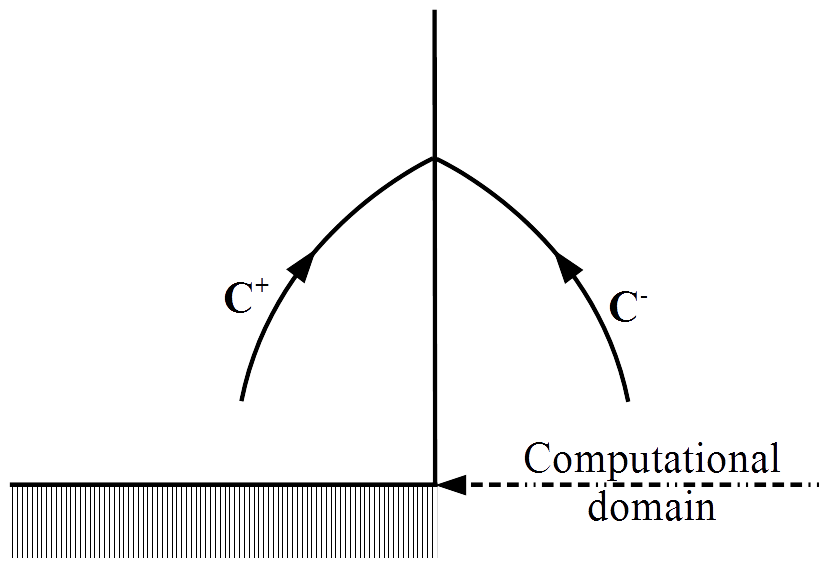
\includegraphics[width=0.8\textwidth]{Figures/AmontFluvial.png}
  \caption{Upstream subcritical flow}
 \end{center}
\end{figure}

Only one of the characteristics comes from outside the domain. The other characteristic (characteristic $C^-$ in this case) comes from inside the domain and carries information to the boundary of the domain. It is therefore necessary to impose the elevation or the flow but not both variables.

\textbf{B) \underline{Upstream supercritical flow}}

\begin{figure}[H]
 \begin{center}
  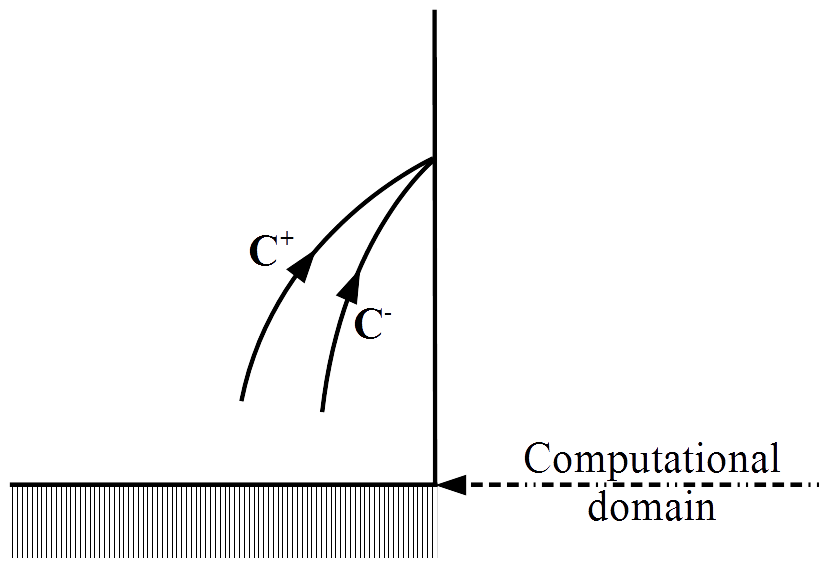
\includegraphics[width=0.8\textwidth]{Figures/AmontTorrentiel.png}
  \caption{Upstream supercritical flow}
 \end{center}
\end{figure}

Both characteristics come from outside the domain. In this case it is necessary to impose the elevation and the flow.

\textbf{C) \underline{Downstream subcritical flow}}

\begin{figure}[H]
 \begin{center}
  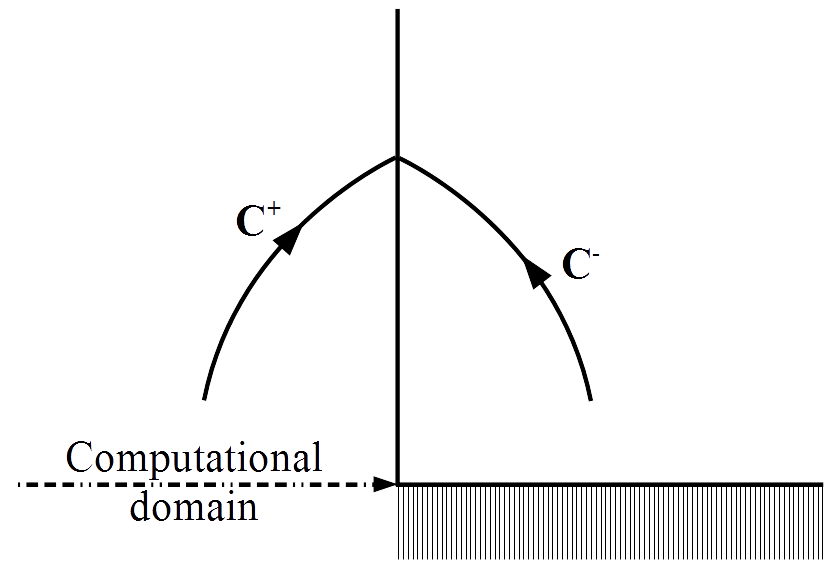
\includegraphics[width=0.8\textwidth]{Figures/AvalFluvial.png}
  \caption{Downstream subcritical flow}
 \end{center}
\end{figure}

These are the same conditions as for upstream subcritical flow. Only one of the variables therefore has to be imposed (either the elevation or the flow). In practice, the elevation is often chosen.

\textbf{D) \underline{Downstream supercritical flow}}

\begin{figure}[H]
 \begin{center}
  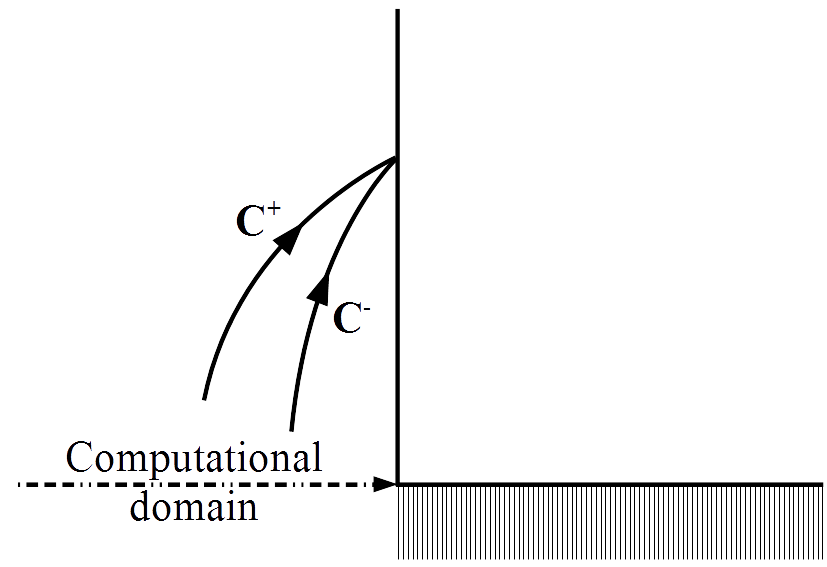
\includegraphics[width=0.8\textwidth]{Figures/AvalTorrentiel.png}
  \caption{Downstream supercritical flow}
 \end{center}
\end{figure}

Both characteristics come from inside the domain. No extra information is required.

The following table summarises the scenarios described above.

\begin{table}[h]
\centering
\caption{Type of flow and upstream/downstream boundary conditions}
\begin{tabular}{c|c|c}
  &\textbf{Subcritical} & \textbf{Supercritical} \\
  \hline
  Upstream & Elevation or Flow & Elevation \textbf{and} Flow \\
  Downstream & Elevation or Flow & nothing \\
  \hline
 \end{tabular}
 \label{TabCL}
\end{table}

%...............................................................................
\subsubsection{Modelling the boundary conditions}
%...............................................................................

The numerical scheme defined in section \ref{PbHom} assumes that the values for the two variables are known at every time step at the boundary of the domain. This, however, can be conflicting with the scenarios introduced in the previous section and following from the characteristics method.

Initially, it is assumed that the boundary conditions are entirely known. The following will focus on how they are taken into account in the overall scheme.

Let us consider a given flow rate applied upstream of the domain.

\begin{figure}[H]
 \begin{center}
  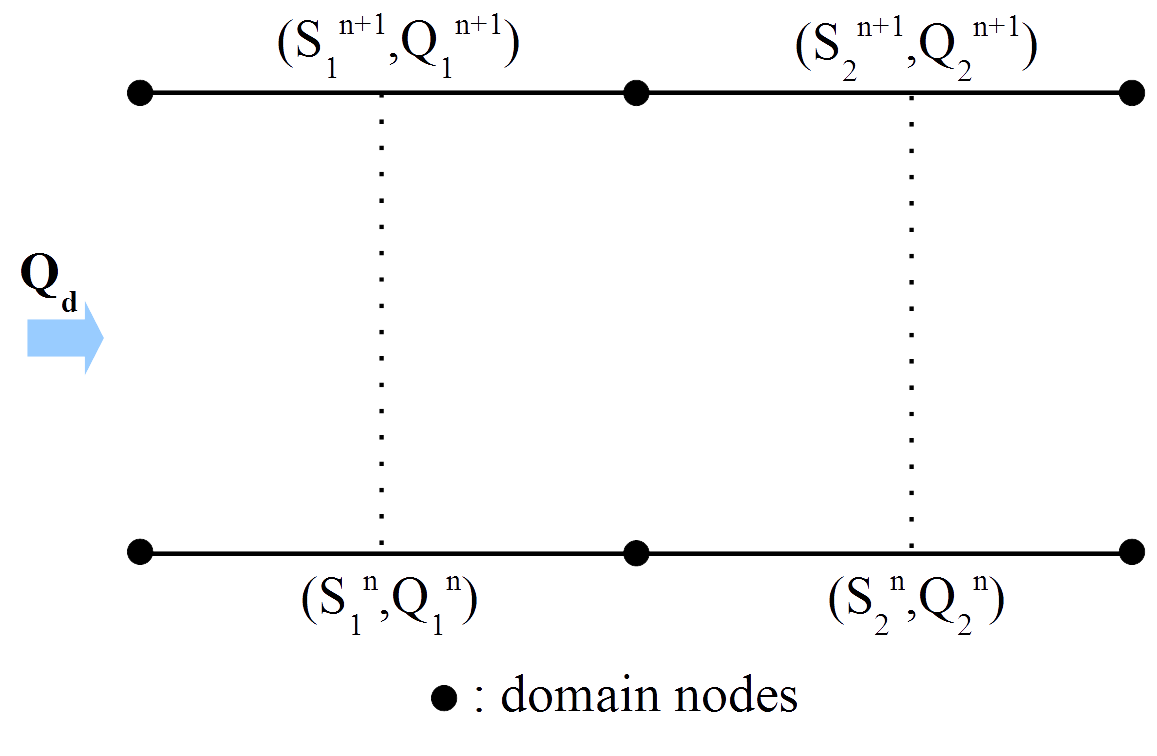
\includegraphics[width=0.8\textwidth]{Figures/NDomaine.png}
  \caption{Downstream supercritical flow}
 \end{center}
\end{figure}

Let us suppose that all the variables are known at the time step $n$.

All the variables at all the nodes in the domain, except those at the boundary, can be evaluated at the time step $n+1$ with the Roe scheme. There are two options to compute $(S_{1}^{n+1},Q_{1}^{n+1})$ :
\begin{itemize}
 \item $(S_{1}^{n+1},Q_{1}^{n+1})$ is computed using the Roe scheme, where the conditions to the left are given by the boundary conditions $(Q_r,S_r)$. It is important to note that the wetted cross-section $S_r$ is not provided by the user but is computed. The following section will introduce how the missing information can be computed;
 \item the first half of the cell is not considered as a cell in the finite volume definition. $(S_{1}^{n+1},Q_{1}^{n+1})$ is set to be equal to the boundary condition $(Q_r,S_r)$. As was the case before, the wetted cross-section will be computed separately.
\end{itemize}

The second method was selected to treat the boundary conditions since it guarantees that the values imposed by the user are found at the first mesh node. This is not guaranteed with the first method.

The various methods available in \mascaret{} to calculate the boundary condition information, independently from the finite volume scheme, are presented in the following sections.

\textbf{A) \underline{Computation of the boundary conditions using the Riemann invariants}}

The principle of this method is very simple and based on the non-\linebreak conservative form of the Saint-Venant equations. It is based on the assumption that the solution is continuous in the immediate vicinity of the boundary conditions. Four possible scenarios can be identified (refer to table \ref{TabCL}) depending on the nature of the flow and on whether considering the upstream or downstream sections.

$\Longrightarrow$ \textsc{Upstream boundary of the domain}

$\rightarrow$ Supercritical flow

The two characteristics enter the domain: it is therefore necessary to provide both the value of the wetted cross-section and that of the flow.

$\rightarrow$ Subcritical flow

The characteristic $C^-$ leaves the domain and carries information from inside the domain towards the upstream boundary condition. This information, the Riemann invariant $f^-$, will be used to supplement the data (wetted cross-section or flow) that the user will have to provide.

This computation is detailed as follows.

$Q_1^{n+1}$ or $S_1^{n+1}$, which are known (provided as input), give a first relationship.

The Riemann invariant $f_{1}^+$ is constant along the characteristic curve $C^-$ resulting from the upstream boundary of the model. This yields a second relationship.

The following system is to be solved :

\begin{equation}
 \left \lbrace
  \begin{array}{l}
    Q_{1}^{n+1} \quad \mbox{or} \quad S_{1}^{n+1} \quad \mbox{known} \\
    \\
    \frac{Q_{1}^{n+1}}{S_{1}^{n+1}} + K(S_{1}^{n+1}) = f_{1}^+
  \end{array}
 \right.
\end{equation}

\begin{itemize}
 \item Imposed flow : the second equation is multiplied by $S_{1}^{n+1}$ to determine $S_{1}^{n+1}$, giving :
   \begin{equation}
     S_{1}^{n+1} K(S_{1}^{n+1}) - f_{1}^+ S_{1}^{n+1} + Q_{1}^{n+1} = 0
   \end{equation}
   This last equation is solved using a Newton method.
 \item Imposed elevation : the computation is much simpler.
   \begin{equation}
      Q_{1}^{n+1} = -S_{1}^{n+1} K(S_{1}^{n+1}) + f_{1}^+ S_{1}^{n+1}
   \end{equation}
\end{itemize}

$\Longrightarrow$ \textsc{Downstream boundary of the domain}

$\rightarrow$ Supercritical flow

Both characteristics leave the domain. No additional information is therefore necessary. The following system is solved :

\begin{equation}
 \left \lbrace
  \begin{array}{l}
    \frac{Q_{N}^{n+1}}{S_{N}^{n+1}} + K(S_{N}^{n+1}) = f_{N}^+ \quad \mbox{with } f_{N}^+ \mbox{ known} \\
    \\
    \frac{Q_{N}^{n+1}}{S_{N}^{n+1}} - K(S_{N}^{n+1}) = f_{N}^- \quad \mbox{with } f_{N}^- \mbox{ known}
  \end{array}
 \right.
\end{equation}

$\rightarrow$ Subcritical flow

This is similar to the upstream subcritical flow scenario.

\begin{CommentBlock}{Note :}
The computation of the boundary conditions using the Riemann invariants is satisfactory and respects the theory of the characteristics. Studies have, however, indicated that this method gives significant errors in cases of small Froude number flows. This is attributed to the fact that the dominant term in the equation is then $SK(S)$ where $K(S)$ is a non-linear function which had to be tabulated (vertical discretisation). To mitigate this major shortcoming for subcritical flows, other methods have been introduced, which are based on a finite difference discretisation of the continuity or momentum equations.
\end{CommentBlock}

\textbf{B) \underline{Computation of the boundary conditions using the Saint-Venant equations}}

This is only relevant for subcritical flows.

$\Longrightarrow$ \textsc{Upstream boundary of the domain}

\begin{itemize}
 \item Imposed flow : the continuity equation is discretised in the simplest possible way using finite differences, to give :
   \begin{equation}
     Q_{1}^{n+1} = Q_r
   \end{equation}
   and :
   \begin{equation}
     \frac{S_{1}^{n+1}-S_{1}^{n}}{\Delta t} + \frac{Q_{2}^n - Q_{1}^n}{\Delta x} = 0
   \end{equation}
   $S_{1}^{n+1}$ is computed using the previous equation.
 \item Imposed elevation : the momentum equation is discretised in a similar way to that used to discretise the continuity equation.
\end{itemize}

$\Longrightarrow$ \textsc{Downstream boundary of the domain}

There is no added difficulty in this case. The approach is similar.

A parameter, called \textit{limit Froude}, which is imposed by the user (refer to user manual) determines the choice of the method to compute the boundary conditions. If the Froude number, upstream or downstream of the domain, is greater than this parameter, the missing information for the boundary conditions will be computed using the Riemann invariants.

\textbf{C) \underline{Representation of a stage-discharge curve}}

So far only the simplest cases have been considered where the elevation or the flow is imposed. For real applications, however, a very useful boundary condition is a \textit{stage-discharge curve} : the elevation and the flow are not known explicitly but are interlinked with a relationship $Z = f(Q)$. The system with two equations and two unknowns is solved to obtain the value of the flow and of the elevation at the domain boundaries. The only difference with the previous cases is that the first equation is not straightforward any more.

\textbf{D) \underline{Representation of a free downstream flow}}

The methods introduced in the previous sections make it possible to compute missing information in the case of subcritical flows but it is still necessary to provide at least the elevation or the flow. This is difficult for flood wave computations where it is impossible for the user to know the elevation or the flow at the downstream boundary of the domain. To address this, it was tried to represent a \textit{free downstream flow}. In this case the user does not provide any boundary condition, these are computed using values from the previous time step only. It is clear that this representation is not correct in consideration of the characteristics method applied to the Saint-Venant equations. The purpose of this representation is not to provide a correct flow for the boundary condition but to let the flood wave leave the domain without influencing too much the flow within the domain.

To obtain a \textit{free downstream flow}, the two variables wetted cross-section and flow rate are moved along at the flow speed.

For flood wave computations it is recommended that the downstream boundary condition for the computational domain is located at least 30 km downstream of the last computational point in order not to disrupt the characteristics at this point. It is strongly advised not to use this type of boundary condition for any other type of computation.

%...............................................................................
\subsection{Dry areas}
%...............................................................................

For applications such as flood waves, it is necessary to be able to model dry areas and the propagation of a front on dry areas. From a numerical viewpoint, the following problems arise :
\begin{itemize}
 \item definition of a flow regime in the dry area because speed is not defined;
 \item propagation of a front on dry areas.
\end{itemize}

The main objective with this problem is to calculate a good propagation velocity of the front since this information is paramount to flood wave computations.

To treat this problem with the Roe scheme, a threshold had to be introduced for the water depth. Using this approach the correct propagation velocity was found on simple test cases where an analytical solution exists \cite{GOUTAL97}. The drawback with this approach is that the perfect conservativity inherent to the finite volumes is then lost. For flood wave computations, the Roe scheme was retained but this entails a strict control of the conservativity.

It should be noted that, within the IAHR work group on numerical methods for flood waves on dry ground, all the teams face the same difficulties.
One of the only schemes that does not have this problem is the so-called equilibrium scheme, developed at the university of Bordeaux by Professor Leroux's team \cite{LECOZ96}\cite{BON97}.

It will be necessary to consider other approaches than that of the threshold depth in the future, but it is a satisfactory solution in the meantime.

%-------------------------------------------------------------------------------
\section{Representation of more complex physical phenomena}
\label{ModelCplx}
%-------------------------------------------------------------------------------

%...............................................................................
\subsection{Introduction to the modelling of compound channels}
%...............................................................................

The transcritical engine of \mascaret{} treats flows in compound channels made up of a low flow channel (river bed) and a high flow channel (floodplain), but storage zones are not considered.

\begin{figure}[H]
 \begin{center}
  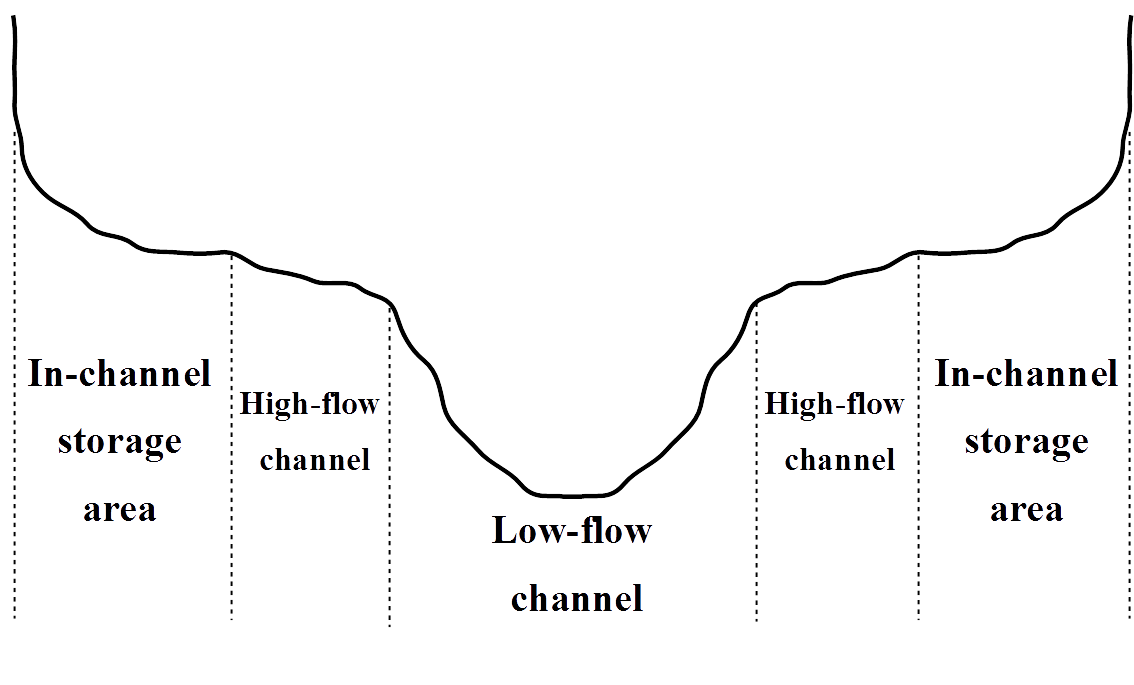
\includegraphics[width=\textwidth]{Figures/Lits.png}
  \caption{Channels and storage sections}
 \end{center}
\end{figure}

The \emph{Debord} formulation was selected to model the low flow and high flow channels such that the subcritical and transcritical engines are as much compatible as possible.

%...............................................................................
\subsubsection{Reminder}
%...............................................................................

The system of equations to solve can now be written as :

\begin{equation}
 \label{SyEQ}
 \left \lbrace
  \begin{array}{l}
    \frac{\partial S}{\partial t} + \frac{\partial Q}{\partial x} = q_l - \frac{\partial S_s}{\partial t} \\
    \\
    \frac{\partial Q}{\partial t} + \frac{\partial}{\partial x} \left ( \frac{Q_{m}^2}{S_m} + \frac{Q_{M}^2}{S_M} + P \right ) \\
    \\
    \quad = g \int_{0}^y \left ( \frac{\partial S}{\partial x}\right )_y \, dy - g S \frac{d Z_f}{d x} - g (S_m J_m + S_M J_M)
  \end{array}
 \right.
\end{equation}

with :

\begin{itemize}
 \item $q_l$ the inflow and $S_s$ the storage section;
 \item $S = S_m + S_M$ and $Q = Q_m + Q_M$;
 \item $\sqrt{J_m} = \frac{Q_m}{D_m}$ and $\sqrt{J_M} = \frac{Q_M}{D_M}$;
 \item $D_m = K_m S_m R_{m}^{2/3}$ and $D_M = K_M S_M R_{M}^{2/3}$ are the conveyances in the river bed and in the floodplain respectively, and depend on the free surface elevation.
\end{itemize}

This system is similar to the Saint-Venant equations in the case of a single channel with the overall slope $J$ defined by means of the relation :

\begin{equation}
 S J = S_m J_m + S_M J_M
\end{equation}

and with the $\beta$ coefficient no longer equal to 1 (as in a river bed), but satisfying the relation :

\begin{equation}
 \beta \frac{Q^2}{S} = \frac{Q_{m}^2}{S_m} + \frac{Q_{M}^2}{S_M}
\end{equation}

\begin{CommentBlock}{Note :}
the $\beta$ coefficient is greater than or equal to 1.
\end{CommentBlock}

%...............................................................................
\subsubsection{The \emph{Debord} formulation}
%...............................................................................

The system of equations (\ref{SyEQ}) is not complete and a closing relation is necessary. Various solutions have been proposed to represent the composition of the two channels. The \emph{Debord} formulation was eventually retained to be compatible with the subcritical engine (refer to section \ref{ModDeb}) and following feedback from various applications of this formulation.

Given :

\begin{equation}
 \eta = \frac{Q_m}{Q_M}
\end{equation}

With the \emph{Debord} formulation :

\begin{equation}
 \eta = \frac{A}{\displaystyle \sqrt{1+\frac{S_m}{S_M}}(1-A^2)} \frac{D_m}{D_M}
\end{equation}

where $A$ is a constant of the \emph{Debord} formulation, computed with :

\begin{equation}
 \left \lbrace
  \begin{array}{l}
    A = \frac{1-A_0}{2}\cos \left ( \frac{\pi r}{0.3} \right ) + \frac{1+A_0}{2} \quad \mbox{for } r=\frac{R_M}{R_m} \in [0,0.3] \\
    \\
    A = A_0 = 0.9 \left ( \frac{K_m}{K_M} \right )^{-1/6} \quad \mbox{for } r > 0.3
  \end{array}
 \right.
\end{equation}

%...............................................................................
\subsubsection{Implementation in the transcritical engine}
%...............................................................................

The equations for compound channels only differ from those for single channels by the $\beta$ term and the form of the source term related to friction. The resolution of this system is therefore formally identical to that treated previously.

The \emph{Debord} formulation makes it possible to write $\beta$ in the form $\beta(S,x)$. This gives an additional unknown function.

For simplicity, the $\beta$ function will be taken into account explicitly. The momentum equation to be solved at time $n+1$ is therefore :

\begin{equation}
 \frac{\partial Q}{\partial t} + \frac{\partial}{\partial x} \left ( \beta^n \frac{Q^2}{S} + P \right ) = g \int_{0}^y \left ( \frac{\partial S}{\partial x} \right )_y \, dy - g S \frac{d Z_f}{dx} -g S J
\end{equation}

It is a partial derivative equation for which the $\beta$ coefficient is variable in time.

The advection system is unconditionally hyperbolic because $\beta$ is greater than or equal to 1. The Riemann problem is solved in a similar way to that related to the Saint-Venant equations for a single channel; the eigenvalues for the system are modified. They become : $\beta u + c'$ and $\beta u - c'$ with : $c' = \sqrt{\frac{\partial P}{\partial S} + u^2(\beta^2 - \beta)}$. The Roe variables remain unchanged.

The representation of friction in this case is exactly identical to that in the case of a single channel; the generalised conveyance takes into account both the river bed and the floodplain, and can be discretised along the vertical in a similar way to the conveyance of the low flow channel.

\begin{CommentBlock}{Note 1 :}
The fact that the $\beta$ term is considered as a forcing function, varying with each time step, simplifies considerably the implementation of the method. This assumption is partly justified because flows in compound channels are generally evolving slowly.
\end{CommentBlock}

\begin{CommentBlock}{Note 2 :}
Conservation properties are lost when modelling compound channels. These properties made it possible to reach a steady state with constant flow. In all the cases studied to date, variations in the flow of the order of $2$ to $3\%$ of the total flow have been observed when a stationary state is reached.
\end{CommentBlock}

%...............................................................................
\subsection{Confluence}
%...............................................................................

A new method has been developed to model confluences. A detailed description can be found in document \cite{MAUREL96} together with validation test cases. The following paragraph summarises the method.

It can be assumed that the 2D Saint-Venant equations replace the 1D equations to represent the flow locally, at and around the junction. It can then be considered that the total domain (main valley + tributary) is the overlap of two sub-domains, where the first sub-domain consists in three 1D reaches (the one-dimensional Saint-Venant equations are supposed to be valid in this case) and where the second sub-domain is the zone around the junction (the two-dimensional equations are supposed to be valid in that case). Modelling the confluence therefore amounts to performing a 1D-2D coupling between the two sub-domains. The 2D Saint-Venant equations are solved using a finite volume module equivalent to that used in 1D (Roe scheme). This module has numerical schemes similar to those used in \mascaret{}. This last point together with the fact that such schemes are explicit has the advantage of facilitating the coupling procedure.

A two-dimensional model usually requires a fine discretisation of the geometry. For flood wave studies, it would not be practical to create a local 2D model for every tributary in a valley, with detailed representation of the geometry and a fine mesh. A simple tool that automate this process is considered as the best approach.
This is why it was decided that the one-dimensional software generates automatically the 2D domain representative of the confluence and the associated mesh. A 12 cells mesh is created by default.

\begin{figure}[H]
 \begin{center}
  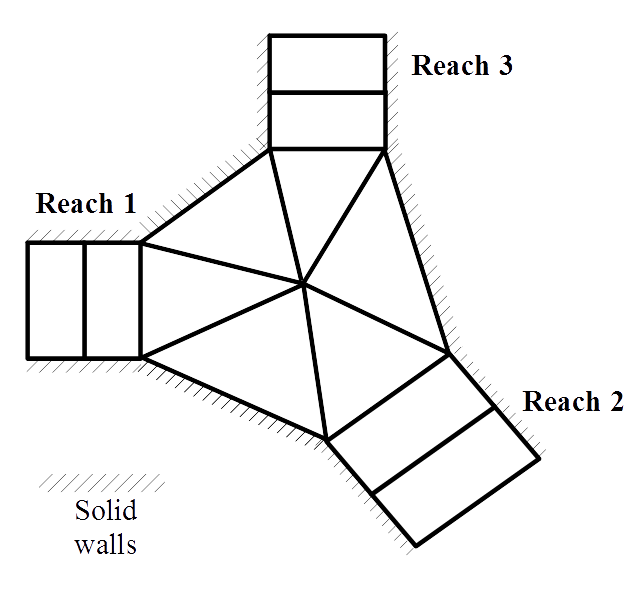
\includegraphics[width=0.8\textwidth]{Figures/ConfPar.png}
  \caption{2D confluence}
 \end{center}
\end{figure}

%...............................................................................
\subsubsection{1D-2D coupling}
%...............................................................................

In the one-dimensional model, the aim is to compute the value of $(S_1,Q_1)$ at the boundary of each 1D reach linked to the confluence. This is equivalent to defining the 1D-2D coupling.

The coupling is done by overlapping domains, i.e. the boundary points of the 2D model are located inside the 1D model. For illustrative purposes, the following figure shows the overlap between the 2D model and the three 1D reaches.

It is assumed that the boundaries of the 1D model, where reaches $B_1$, $B_2$, $B_3$ are located, are represented in the 2D model by cells $A$, $B$, $C$ respectively. Cells $a$, $b$, $c$, at the boundaries of the 2D model, represent the cells close to the ends to each 1D reach. The 1D-2D coupling is then done by exchange of boundary conditions.

\begin{figure}[H]
 \begin{center}
  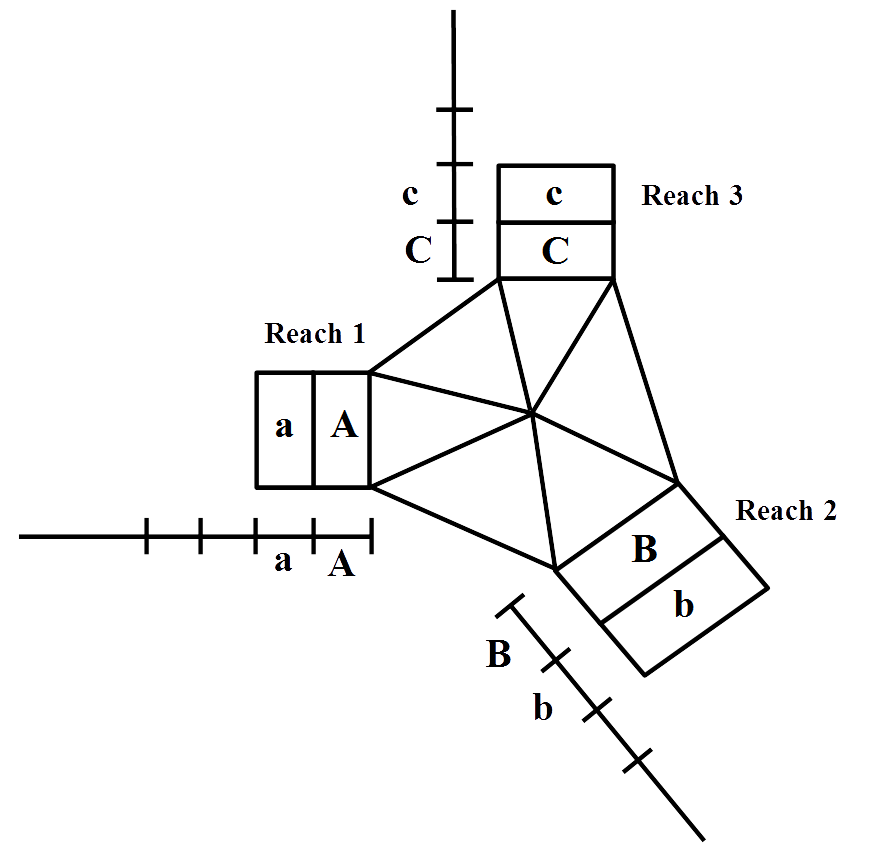
\includegraphics[width=0.8\textwidth]{Figures/ConfPar2.png}
  \caption{1D-2D overlap}
 \end{center}
\end{figure}

A computation can be described as follows :

The state in each 1D reach: $B_1$, $B_2$, $B_3$ and in the 2D confluence is assumed to be known at time $n$. The state at time $n+1$ is determined in four steps :
\begin{itemize}
 \item \textbf{Step 1 :} computation of the state at the confluence (except for the three boundary cells $a$, $b$ and $c$). This stage is carried out with a 2D Roe scheme. The scheme is explicit; the boundary conditions at time $n+1$ are not required, only the conditions for state $n$ everywhere;
 \item \textbf{Step 2 :} computation of the state inside each reach (except for boundary cells $A$, $B$, $C$). This stage is carried out with a 1D Roe scheme for the same reasons and in the same way as previously discussed;
 \item \textbf{Step 3 :} computation of $S_1$, $Q_1$ in each reach. These are the values of $S$ and $Q$ in $A$, $B$, $C$. These values have been computed at step 1. The free surface level is maintained from one model to the other. The computed flow values, however, are two-dimensional. The flow vector is therefore projected along the normal to the free boundary in order to obtain a one-dimensional value.
 \item \textbf{Step 4 :} computation of the boundary conditions for the 2D model. These were determined at step 2 in the cells adjacent to the ends of each reach. Similarly to the previous step, the free surface level is maintained from the 1D model to the 2D model. Furthermore, the flow direction is assumed to be that of the normal to the free boundary in order to have a two-dimensional flow.
\end{itemize}

Finally, the complete state of the one-dimensional model (reaches $B_1$, $B_2$, $B_3$) and of the two-dimensional model (the confluence) is computed at time $n+1$.

The use of a finite volume scheme in the 2D model makes modelling of the confluence a priori conservative. This is not entirely true because a projection of the flow is used to go from the 2D state to the 1D state and this introduces a source of non-conservatism to the momentum.

%...............................................................................
\subsubsection{Adapting the 1D geometry to the 2D model}
%...............................................................................

Now that the coupling method has been defined, all that remains is to describe the 2D model selected to represent the junction. Initially, the simple case of rectangular channels is considered. Then the method is extended to real geometries.

$\Longrightarrow$ Rectangular channels

The geometry of the junction is discretised using twelve cells such that it is reasonnable close to the real geometry.

\begin{itemize}
 \item[*] For each tributary, the coordinates of the boundary point on the hydraulic axis are provided, as well as the angle this 1D reach forms with a set direction. These are the only external data specific to the confluence. They are determined only from geometrical criteria;
  \begin{figure}[H]
    \begin{center}
     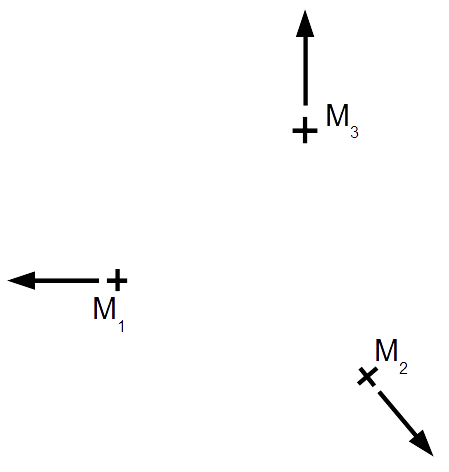
\includegraphics[width=0.5\textwidth]{Figures/cr1.png}
    \end{center}
  \end{figure}

 \item[*] for each tributary $i$, a segment can be traced with length $L_i$ (the width of the channel, independent from the definition of the confluence, and coming directly from the geometry of the 1D model). This segment is normal to the angle previously set;
  \begin{figure}[H]
    \begin{center}
     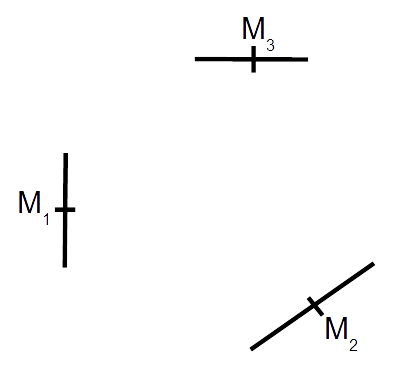
\includegraphics[width=0.5\textwidth]{Figures/cr2.png}
    \end{center}
  \end{figure}

 \item[*] these segments are then joined up by walls. The three segments previously defined together with the walls form a hexagon at the junction;
   \begin{figure}[H]
    \begin{center}
     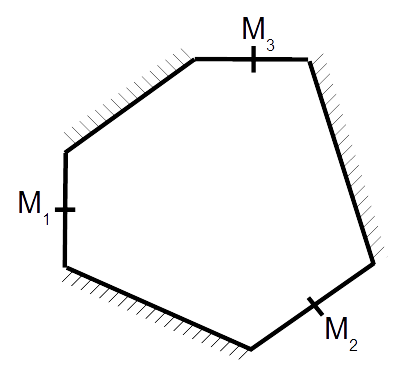
\includegraphics[width=0.5\textwidth]{Figures/cr3.png}
    \end{center}
  \end{figure}

 \item[*] $G$ is the centre of gravity of the hexagon. Inside the hexagon, six triangles are formed with $G$ as a common vertex;
  \begin{figure}[H]
    \begin{center}
     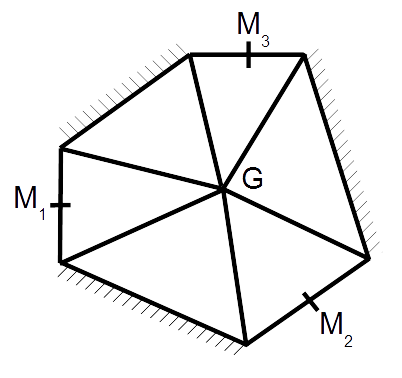
\includegraphics[width=0.5\textwidth]{Figures/cr4.png}
    \end{center}
  \end{figure}

 \item[*] the cells in the 1D-2D overlapping area are rectangles with sides $L_i$ and $DX_i$, the size of the 1D cell in each reach;
  \begin{figure}[H]
    \begin{center}
     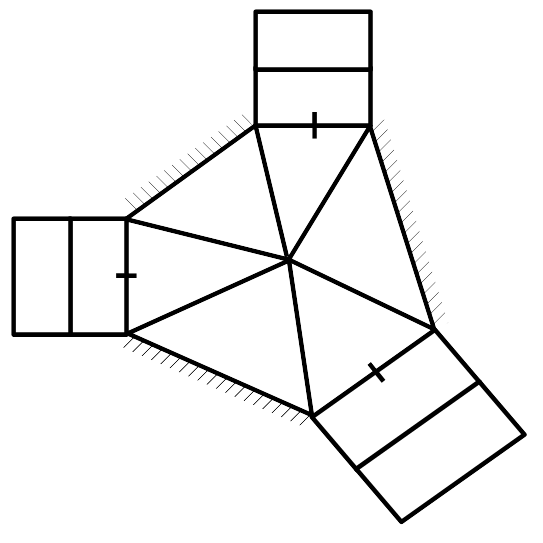
\includegraphics[width=0.5\textwidth]{Figures/cr5.png}
    \end{center}
  \end{figure}

 \item[*] last but not least, the bottom elevation in each cell is set as follows :
   \begin{itemize}
     \item for the six overlapping cells, it is the elevation of the 1D cell, $Z_{f1D}$;
     \item inside the hexagon, the elevation of $G$ ($Z_{fG}$) is taken to be the arithmetic mean of those in the three neighbouring 1D-2D overlapping cells. The three cells that have an edge in common with the overlapping cells (thus no walls) have an elevation $Z_{f2D}$ defined by : $Z_{f2D} = \frac{2Z_{f1D}+Z_{fG}}{3}$ where $Z_{f1D}$ is the elevation of the adjacent 1D cell;
     \item for each of the other three cells, the bottom elevation is assumed to be the average of the elevation at the two adjacent cells.
   \end{itemize}
\end{itemize}

This parameterisation has the advantage that it only requires few specific parameters: the coordinates of points $M_i$ and the relative orientation of each reach. These are purely geometrical parameters, which are easy to determine. The remainder of the information comes directly from the 1D parameterisation (geometry of the cross-reach profiles) and from the state of each reach.

The geometry thus defined takes into account :

\begin{itemize}
 \item the importance of the extent of the zone of confluence, through the relative position of the three points $M_i$;
 \item the orientation of each reach, through the angles provided for each $M_i$;
 \item the width of each channel, since it is transferred in the 2D model from the 1D state;
 \item the bottom variations, since the elevation of the overlapping cells is that of the 1D cells. Inside the hexagon, the bottom elevations vary smoothly.
\end{itemize}

$\Longrightarrow$ Real geometry channels

A difficulty arises in the case of a real geometry. A cross-section will be discretised using only one cell in the 2D model. This 2D cell represents a rectangular profile since the bottom of a cell is flat with the $P_0$ discretisation used here. This point was obviously trivial in the previous case, but must now be addressed specifically.

The problem is to find the rectangular geometry equivalent to the real geometry, in the sense that the flows represented in each model must be as close as possible. A 1D-2D transformation must therefore be defined and the following was retained :
\begin{itemize}
 \item the bottom elevation $Z_f$ is preserved;
 \item the free surface elevation $Z$ is preserved (thus $Y$, the water depth, is also preserved);
 \item the discharge $Q$ is preserved;
 \item the velocity $V$ is preserved.
\end{itemize}

It is thus necessary to preserve the wetted cross-section $S$. The depth being fixed by the first two points, the width can be deduced from :

\begin{equation}
 L_{2D} = \frac{S_{1D}}{Y}
\end{equation}

This cell width is likely to change when the depth varies. The grid must therefore be updated in a regular way at each time step.

%...............................................................................
\subsection{Singularities}
%...............................................................................

When a flood wave propagates in a real valley, dams located downstream of the main dam need to be taken into account. These structures can respond in several possible ways: instantaneous failure when the wave arrives or spilling over the crest of the structure. In the second case, the dam can be modelled in two different ways :

\begin{itemize}
 \item direct representation in the geometry. This solution, however, would require a very fine grid in the immediate proximity of the structure since the slopes of the faces are steep upstream and downstream of the structure. This would strongly constrain the time step for the whole computational domain;
 \item representation as a singularity. With this option the dam is not treated as a regular node in the numerical scheme. Instead, a specific relationship relates the water upstream and downstream of the dam.
\end{itemize}

The method used to model a singularity in the case of a finite volume scheme will be introduced in the remainder of this section.

It is considered that a singularity is defined by a relation linking the conveying flow $Q_s$ through this singularity to the upstream and downstream water levels. This relation depends on the physical and hydraulic characteristics of the structure.

A part of the domain is represented in the figure below.

A singularity has to be located at the interface between 2 cells. The flow through this interface is defined by : $Q_s = f(Z_{i-1},Z_i)$.

\begin{figure}[H]
    \begin{center}
     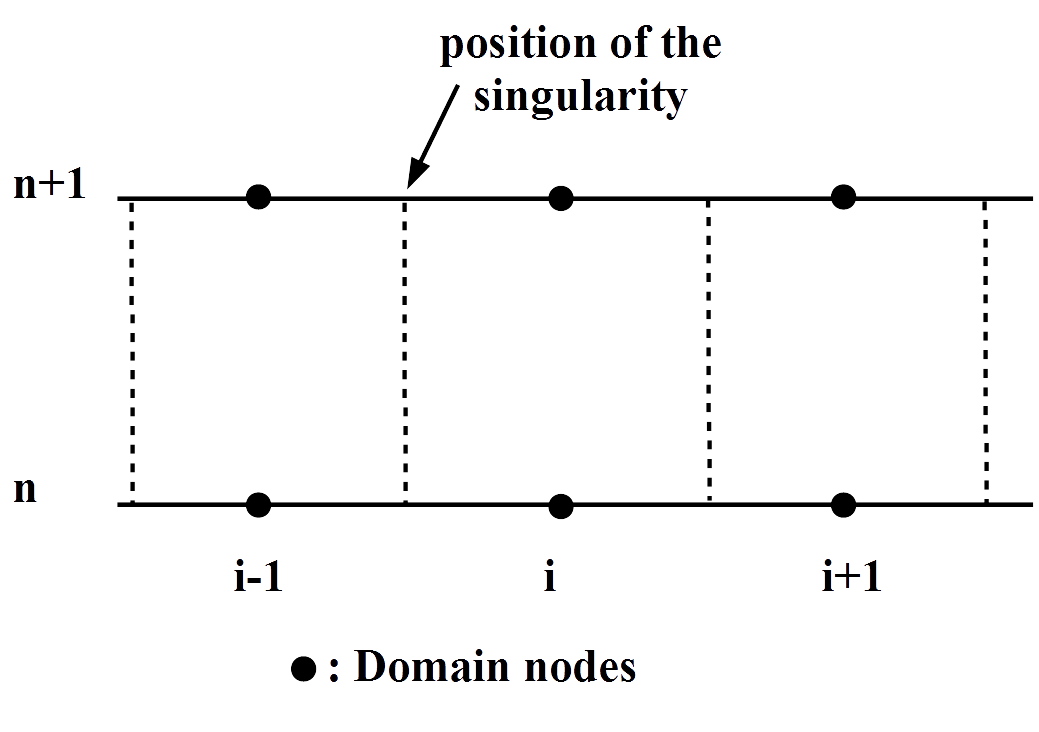
\includegraphics[width=0.8\textwidth]{Figures/posSing.png}
    \end{center}
\end{figure}

With a finite volume scheme, the hydraulic state in cells $i$ and $i-1$ at time $n+1$ depends on the fluxes at the interface of both cells.

For cell $i$ (respectively $i-1$), the flux to the right (respectively to the left) will be that computed by the scheme defined in section $n$. The mass and momentum fluxes at the interface between cell $i$ and cell $i-1$, however, will not be that of Roe, but the analytical flux explicitly computed using the relation defining the singularity.

\textbf{\underline{For cell $i$}}

Mass flux to the left : $Q_s =f(Z_{i-1}^n,Z_{i}^n)$

Momentum flux to the left : $\frac{Q_{s}^2}{S_{i}^n} + P(S_{i}^n)$

\textbf{\underline{For cell $i-1$}}

Mass flux to the right : $Q_s =f(Z_{i-1}^n,Z_{i}^n)$

Momentum flux to the right : $\frac{Q_{s}^2}{S_{i-1}^n} + P(S_{i-1}^n)$

\begin{CommentBlock}{Note :}
\begin{itemize}
 \item mass is therefore conserved. Momentum, however, is no longer conserved;
 \item at the very beginning of the spill, the wetted cross-section downstream of the singularity is very small. This implies very strong flows and consequently numerical problems (instabilities). In this situation, only the pressure term is kept in the momentum flux equation;
 \item this representation allows all types of singularities to be taken into account. All that is required is the function linking the discharge to the upstream and downstream elevations.
\end{itemize}
\end{CommentBlock}

%...............................................................................
\subsection{Eroding dams}
%...............................................................................

The transcritical engine of \mascaret{} makes it possible to model erosion, by overflow, of the gravity dams located downstream of the principal dam.

The selected method is largely inspired from that implemented in the \texttt{EROSIF} solver \cite{BENSLAMA95}. \texttt{EROSIF} computes the evolution of a breach in an embankment as well as the downstream hydrograph resulting from the progressive failure.

Within \mascaret{}, a dam eroding by overflow is treated as a spilling dam with a crest elevation variable in time.

\begin{figure}[H]
    \begin{center}
     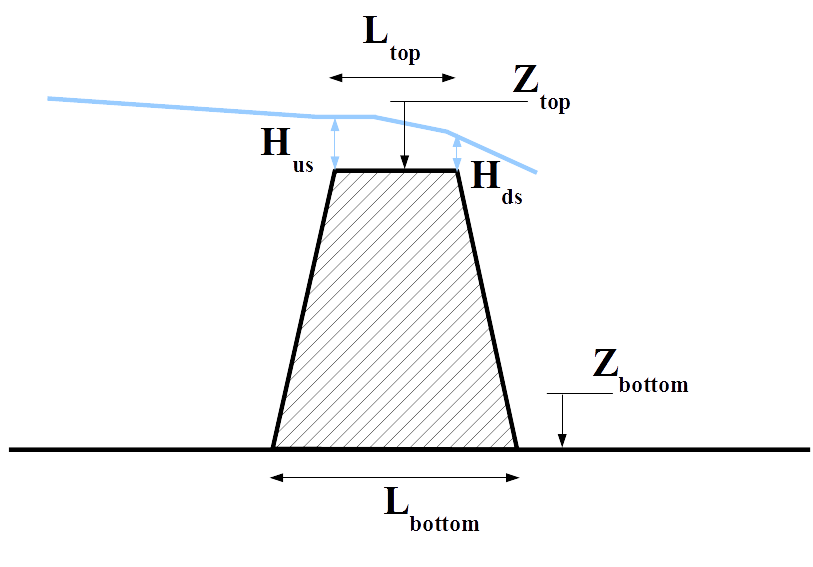
\includegraphics[width=0.8\textwidth]{Figures/BarPds.png}
     \caption{Modelling notations}
    \end{center}
\end{figure}

Upstream of the dam, the hydraulic conditions are assumed to be identical to those computed by the transcritical engine in the cell immediately upstream of the dam at the previous time step.

Downstream of the dam, a critical condition is imposed. The flow across the whole structure is assumed to be equal to the upstream flow.

The evolution of the elevation of the dam crest is given by the equation :

\begin{equation}
 (1-p) \frac{dZ_{top}}{dt} = - \frac{dQ_s}{dx} = - \frac{Q_{s_{d/s}}-Q_{s_{u/s}}}{L_{top}}
\end{equation}

where $p$ is the porosity of the material (usually taken as 0.4), $Q_{s_{u/s}}$ et $Q_{s_{d/s}}$ are the sediment transport rate respectively upstream and downstream of the erosion channel, and calculated using the of Meyer Peter Muller formulation, i.e. :

\begin{equation}
 Q_s = \frac{8}{g \sqrt{\rho}(\rho_s - \rho)}(\tau - \tau_c)^{1.5}
\end{equation}

with :
\begin{itemize}
 \item $\tau$ the global hydrodynamic stress (Manning Strickler formulation);
 \item $\tau_c$ the critical shear stress : $0.05 . (\rho_s - \rho).g.d_{50}$;
 \item $\rho_s$ the density of the sediment;
 \item $\rho$ the density of water;
 \item $d_{50}$ the median diameter of the material.
\end{itemize}

All these equations make it possible to compute $Z_{top}$, the crest elevation. Erosion is limited at the bottom by the elevation $Z_{low}$.

%...............................................................................
\subsection{Broad-crested and sharp-crested weirs}
\label{LoiSeuilMinceEpais}
%...............................................................................

This section presents the methodology for modelling singularities of the type broad-crested or sharp-crested weirs, as implemented in the transcritical and subcritical engines. For the other singularities, the pair (flow, elevation) is directly determined by interpolation from a discretised table, provided by the user.

The laws for weirs implemented in the transcritical and subcritical engines give the user a choice between two types of weirs: broad-crested or sharp-crested weirs. These two laws differ only when the weir is drowned, in particular with the flow conditions and the drowning coefficient.

The validation tests carried out in the case of a sharp-crested weir are detailed in \cite{GOUTAL03}.

%...............................................................................
\subsubsection{Broad-crested or sharp-crested free flow weir}
%...............................................................................

\begin{figure}[H]
    \begin{center}
     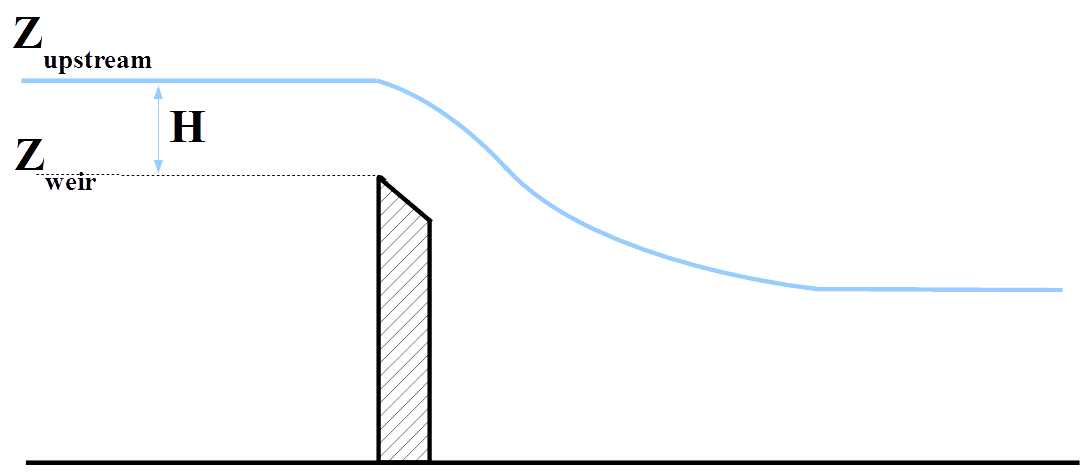
\includegraphics[width=0.8\textwidth]{Figures/Sden.png}
    \end{center}
\end{figure}

The flow over a broad-crested or sharp-crested free flow weir can be expressed as :

\begin{equation}
 \label{debSeuil}
 Q = C L H \sqrt{2 g H}
\end{equation}

where:

\begin{itemize}
 \item $H$ is the water head upstream of the weir (the approach velocity is ignored) : $H = Z_{u/s} - Z_{weir}$;
 \item $g$ is the gravity;
 \item $L$ is the width of the weir;
 \item $C$ is a discharge coefficient which depends on contraction effects and on approximations made when writing the formula (\ref{debSeuil}) : for example the fact that the approach velocity is not accounted for. This coefficient, $C$, is determined by the user and can result from a calibration of the model.
\end{itemize}

More details on how the previous formula was established are given in \cite{CARLIER87}.

The laws are identical when the weirs are not drowned. When they are drowned, however, the laws differ with the type of weir (conditions and drowning coefficient).

%...............................................................................
\subsubsection{Drowned weir}
%...............................................................................

\begin{figure}[H]
    \begin{center}
     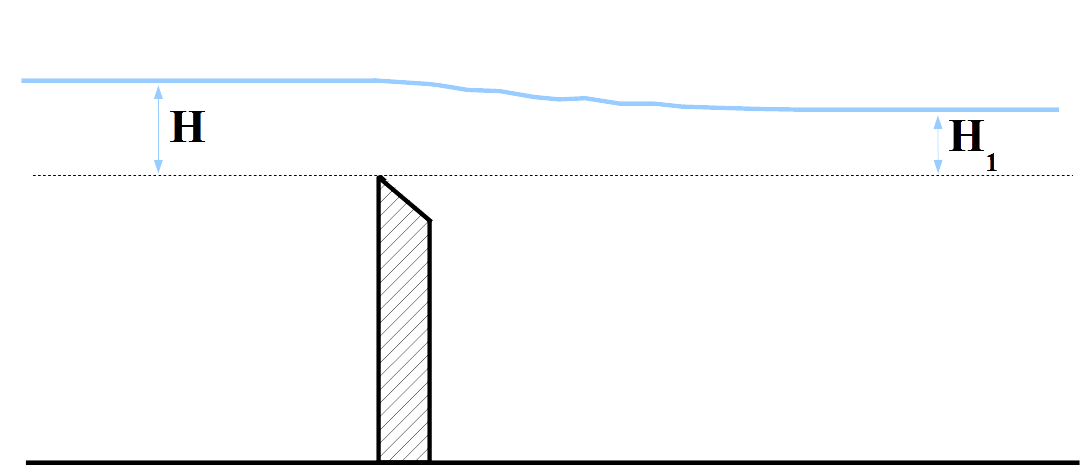
\includegraphics[width=0.8\textwidth]{Figures/Snoy.png}
    \end{center}
\end{figure}

A weir is considered drowned when the upstream elevation is influenced by the downstream elevation. The discharge for a broad-crested or sharp-crested drowned weir can be expressed in a similar way to that for a drowned weir. Only the discharge coefficient, $C$, is modified to take into account the influence of the downstream reach on the discharge over the weir. A drowning coefficient, $K$, is defined as :

\begin{equation}
 K = \frac{Q_{\mbox{drowned flow}}}{Q_{\mbox{free flow}}}
\end{equation}

The discharge over the drowned weir is therefore expressed as :

\begin{equation}
 \label{sny}
 Q = K C L H \sqrt{2 g H}
\end{equation}

where :
\begin{itemize}
 \item $K$ is a coefficient which depends on the ratio $\frac{H_1}{H}$ and the type of weir;
 \item $H=Z_{u/s}-Z_{weir}$ et $H_1 = Z_{d/s}-Z_{weir}$;
 \item $C$ is the discharge coefficient defined above for the drowned weir.
\end{itemize}

$\Longrightarrow$ Broad-crested drowned weir

For a broad-crested weir, the downstream elevation does not influence the discharge over the sill when $H_1$ is lower than $0.8H$ (even though the elevation of the downstream reach may be higher than the weir crest elevation). This is linked to the presence of a critical section over the weir.

The drowning coefficient $K$ in the formula (\ref{sny}) is that typically used for broad-crested weirs. It can be expressed as :

\begin{equation}
 \left \lbrace
  \begin{array}{l}
    K = -25 \left ( \frac{H_1}{H} \right )^2 + 40 \left ( \frac{H_1}{H} \right ) - 15 \quad \mbox{if } \frac{H_1}{H} > 0.8\\
    \\
    K = 1 \quad \mbox{if } \frac{H_1}{H} < 0.8
  \end{array}
 \right.
\end{equation}

$\Longrightarrow$ Sharp-crested drowned weir

For a sharp-crested weir :
\begin{itemize}
 \item if $H_1 < 0$, $K=1$ : the downstream elevation does not influence the discharge over the weir;
 \item if $H_1 > 0$, i.e. as soon as the downstream elevation is higher than that of the weir crest, we have :
   \begin{equation}
     K = \left ( \left ( 1 - \frac{H_1}{H} \right )^{1.5} \right )^{0.385}
   \end{equation}
\end{itemize}

Figure \ref{fig:CFEN} gives the shape of the drowning coefficients as a function of $\frac{H_1}{H}$, for both a broad-crested and a sharp-crested weir.

\begin{figure}[H]
    \begin{center}
     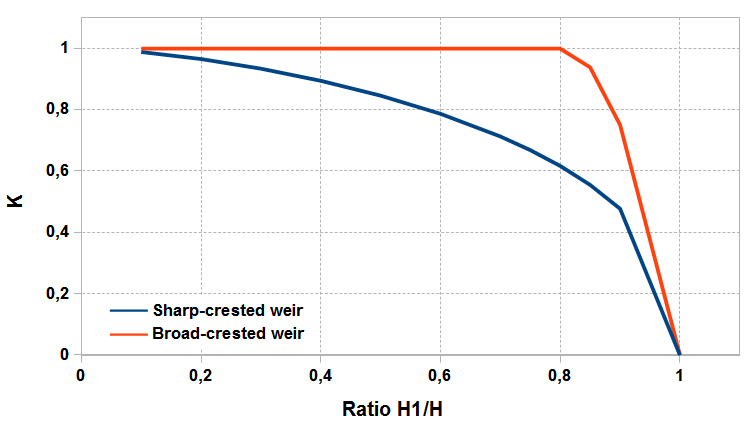
\includegraphics[width=\textwidth]{Figures/CoefEn.png}
     \caption{Drowning coefficient}
     \label{fig:CFEN}
    \end{center}
\end{figure}

%...............................................................................
\subsection{Summary of the treatment of singularities}
\label{BilanSing}
%...............................................................................

There may exist in a river some regions where the Saint-Venant equations do not apply because the assumptions (for example, uniform distribution of the speeds along the vertical) are no longer valid. Flows over weirs, valves etc... are some examples.

The relationships between the elevation and the discharge in the close vicinity of the singularities are then described by explicit laws. The subcritical engines of \mascaret{} can model singularities such as weirs and valves in a river when those are explicitly modelled by hydraulic laws relating the discharge through the singularity, the upstream and downstream elevations and the characteristics of the singularity. Although a number of singularities are implemented in MASCARET, they are not all available for the transcritical engine. The following table lists the various singularities and their availability in the subcritical and transcritical engines.

\begin{table}[H]
\centering
\caption{Singularities modelled in \mascaret{}}
 \label{TBL2}
\begin{tabular}{c|c|c}
  \textbf{Type of singularities} & \textbf{Subcritical engine} & \textbf{Supercritical engine} \\
  \hline
  $Q=f(Z_{d/s})$ & \textbf{yes} & no \\
  $Q=f(Z_{u/s})$ & \textbf{yes} & \textbf{yes} \\
  Law for broad-crested weir & \textbf{yes} & \textbf{yes} \\
  Law for sharp-crested weir & \textbf{yes} & \textbf{yes} \\
  $Z_{u/s}=f(Q)$ & \textbf{yes} & no \\
  $Z_{u/s}=f(Z_{d/s},Q)$ & \textbf{yes} & no \\
  Weir with crest defined by multiple points & \textbf{yes} & no \\
  $Z_{u/s}=f(t)$ & \textbf{yes} & no \\
  Law for valves & \textbf{yes} & no \\
  \hline
 \end{tabular}
\end{table}

%...............................................................................
\subsection{Non-hydrostatic terms}
%...............................................................................

This section presents an extension of the Saint-Venant equations, which considers some of the terms introduced when non-hydrostatic effects are taken into account. The aim is to model physical phenomena such as Favre waves (or undular bores). It should be noted that these developments are only valid for subcritical, unsteady flows with a shallow bed slope. This is derived from work by BRISTEAU et al. \cite{BRISTEAU11}.

The following paragraphs describe the additional terms and their representation within the framework of the transcritical engine in \mascaret{} (finite volume scheme of Roe type). These developments can also be applied without much difficulty to the \REZO{} engine dedicated to subcritical flows. These were the subject of a publication where the reader will find all the necessary explanations \cite{BRISTEAU11}.

The Saint-Venant equations are obtained from the Navier-Stokes equations by making the following assumptions :
\begin{itemize}
  \item long waves (shallow-water);
  \item hydrostatic pressure;
  \item uniform distribution of speeds in the vertical.
\end{itemize}

Let us start from the equations of Euler with 2 dimensions $(x,z)$ to eliminate the constraint of hydrostatic pressure, where $z$ represents the vertical axis and $x$ the horizontal axis. For the purpose of simplicity, friction is neglected.

\begin{eqnarray}
\frac{\partial u}{\partial x} + \frac{\partial w}{\partial z} & = & 0 \label{eq:NS_2d1}\\
\frac{\partial u}{\partial t} + u \frac{\partial u}{\partial x} + w \frac{\partial u}{\partial z} + \frac{\partial p}{\partial x} & = & 0 \label{eq:NS_2d2}\\
\frac{\partial w}{\partial t} + u\frac{\partial w}{\partial x} + w\frac{\partial w}{\partial z} + \frac{\partial p}{\partial z} & = & -g \label{eq:NS_2d3}
\end{eqnarray}

with : $t> t_0, \quad x \in \mathbb{R}$  and $\quad Z_b(x) \leq z \leq Z(x,t)$

$Z(x,t)$ represents the free surface elevation, $\mathbf{u}=(u,w)^T$ is the velocity vector and $p$ the pressure.

The water depth is : $h = Z - Z_b$.

The bed elevation $Z_b$ varies with the curvilinear coordinate $x$ of the river.

% \begin{figure}
%  \begin{center}
%   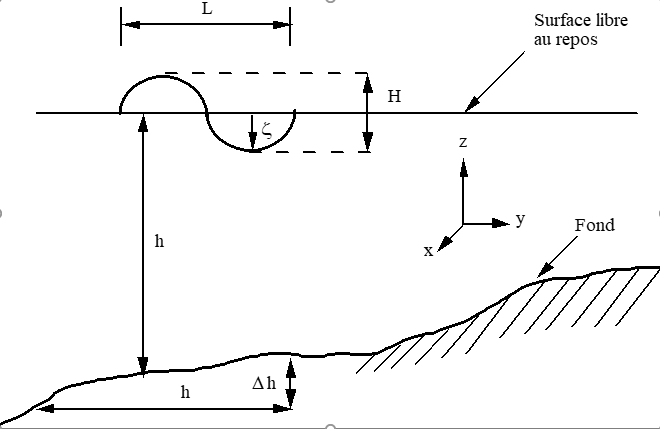
\includegraphics[scale=0.5,angle=0]{notations.png}
%   \caption{Notations: water depth $H(x,t)$, Free surface level $Z(x,t)$ and bottom level $Z_f(x,t)$.}
%   \label{fig:notations}
%  \end{center}
% \end{figure}

The system of equations (\ref{eq:NS_2d1}) to (\ref{eq:NS_2d3}) is supplemented by the following boundary conditions. If $n_s$ is the normal to the free surface and $n_b$ the normal to the bed surface :

\begin{equation}
 n_s = \frac{1}{\displaystyle  \sqrt{1 + \left( \frac{\partial z}{\partial x}\right)^2} }  \left( \begin{array}{c} -\frac{\partial z}{\partial x}\\ \\ 1 \end{array} \right)
\end{equation}

and

\begin{equation}
 n_b = \frac{1}{\displaystyle \sqrt{1 + \left( \frac{\partial z_b}{\partial x}\right)^2}}  \left(\begin{array}{c} -\frac{\partial z_b}{\partial x}\\ \\ 1 \end{array} \right)
\end{equation}

%...............................................................................
\subsubsection{At the free surface}
%...............................................................................

The boundary condition at the free surface is a traditional kinematic condition :
\begin{equation}
\frac{\partial Z}{\partial t} + u_s \frac{\partial Z}{\partial x}
-w_s = 0
\label{eq:free_surf}
\end{equation}
where subscript $s$ indicates the value of the variable at the free surface.

%...............................................................................
\subsubsection{At the bottom}
%...............................................................................

\begin{equation}
 u_f \frac{\partial z_b}{\partial x}-w_f = 0
 \label{eq:bottom}
\end{equation}

where subscript $b$ indicates that the value of the variable is taken at the bottom.

The notations here are the same as those introduced in the previous section about the transcritical engine of \mascaret{}.

\begin{eqnarray}
 S(x,t) & = & \int_{l_{1}}^{l_{2}}h(x,y,t)dy \\
 \bar{u}(x,t) & = & \frac{1}{S(x,t)}\int_{l_{1}}^{l_{2}}\int_{Z_{b}}^{Z(x,t)}u(x,y,z,t)dzdy \\
 Q(x,t) & = & S(x,t)\bar{u}(x,t)
\end{eqnarray}

Integration along the vertical of the continuity equation (\ref{eq:NS_2d1}), with the boundary conditions defined by (\ref{eq:free_surf}) and (\ref{eq:bottom}), gives :

\begin{equation}
  \frac{\partial{S}}{\partial{t}}+\frac{\partial{Q}}{\partial{x}}=0 \label{eq:STV_1d1}\\
\end{equation}

Integration of equation (\ref{eq:NS_2d3}) gives the expression of the pressure.

\begin{equation}
  p(x,z,t)=p^{a}+g(Z(x,t)-z(x,t))+\int_{z}^{Z}{\frac{\partial{w}}{\partial{t}}}dz
\end{equation}

With the assumption that the pressure is hydrostatic, the term which depends on the vertical velocity component is not taken into account. It is also noted that only the term corresponding to the temporal derivative of the vertical velocity component is considered. The advective terms are here neglected. Integration along the vertical of the momentum equation (\ref{eq:NS_2d2}) gives the following equation :

\begin{equation}
\frac{\partial{Q}}{\partial{t}}+\frac{\partial{Q^{2}}}{\partial{x}}+g\int_{l_{1}}^{l_{2}}h\frac{\partial{Z}}{\partial{x}}dy+D =0
\label{eq:mod_cont}
\end{equation}

The friction terms are neglected. $D$ represents part of the non-hydrostatic terms, which are developed in the following section.

%...............................................................................
\subsubsection{Development of the non-hydrostatic terms}
%...............................................................................

\begin{equation}
D=\int_{l_{1}}^{l_{2}}\int_{Z_{b}}^{Z(t)}{\frac{\partial}{\partial{x}}}\left(\int_{z}^{Z(t)}{\frac{\partial{w}}{\partial{t}}dz_{1}}\right)dz
\label{eq:tnh}
\end{equation}

The velocity is such that its divergence equals zero (\ref{eq:NS_2d1}). Combined with the impermeability conditions at the bottom, the following expressions are obtained :

\begin{eqnarray}
w(z) & = & - \frac{\partial}{\partial{x}}\int_{Z_{b}}^{z}udz_1\\
     & = & - \frac{\partial}{\partial{x}}((z-Z_{b})\bar{u})\\
     & = & -(z-Z_{b})\frac{\partial{\bar{u}}}{\partial{x}}+\frac{\partial{Z_b}}{\partial{x}}\bar{u}
\label{expw}
\end{eqnarray}

If the expression for the vertical velocity component is incorporated in the term $D$, representing part of the non-hydrostatic terms, and if the Leibnitz rule is applied to (\ref{eq:tnh}), the following relation is obtained :

\begin{equation}
  D =\int_{l_{1}}^{l_{2}}\int_{Z_{b}}^{Z(t)}\left(\int_{z}^{Z(t)}\frac{\partial^2{w}}{\partial{x}\partial{t}}dz+\left.\frac{\partial{Z(t)}}{\partial{x}}\frac{\partial{w}}{\partial{t}}\right|_s\right)dzdy
\end{equation}

This relation is further developed when replacing the vertical velocity component by its expression (\ref{expw}).

\begin{eqnarray}
  D & = & -\frac{1}{2}\int_{l_{1}}^{l_{2}}\int_{Z_{b}}^{Z(t)}\left[{h}^2-{(z-Z_f)}^2\right]dzdy\frac{\partial^3{\bar{u}}}{\partial{{x}^2}\partial{t}} \\
    & + & 2\int_{l_{1}}^{l_{2}}\int_{Z_{b}}^{Z(t)}(Z-z)\frac{\partial{Z_f}}{\partial{x}}dzdy\frac{\partial^2{\bar{u}}}{\partial{x}\partial{t}} \nonumber \\
    & + & \int_{l_{1}}^{l_{2}}\int_{Z_{b}}^{Z(t)}(Z-z)\frac{\partial^2{Z_f}}{\partial^2{x}}dzdy\frac{\partial{\bar{u}}}{\partial{t}}\nonumber \\ & + & \int_{l_{1}}^{l_{2}}\int_{Z_{b}}^{Z(t)}h\frac{\partial{Z}}{\partial{x}}dzdy\frac{\partial^2{\bar{u}}}{\partial{x}\partial{t}}\nonumber \\
& + & \int_{l_{1}}^{l_{2}}\int_{Z_{b}}^{Z(t)}\frac{\partial{Z}}{\partial{x}}\frac{\partial{Z_f}}{\partial{x}}dzdy\frac{\partial{\bar{u}}}{\partial{t}} \nonumber
\end{eqnarray}

Not all the above terms are taken into account in the transcritical engine of \mascaret{}. Only the dominant term that does not contain bottom gradient terms is kept:

\begin{equation}
-\frac{1}{2}\int_{l_{1}}^{l_{2}}\int_{Z_{b}}^{Z(t)}\left[{h}^2-{(z-z_f)}^2\right]dzdy\frac{\partial^3{\bar{u}}}{\partial{{x}^2}\partial{t}}
\end{equation}

The double integral is expressed as follows :
\begin{eqnarray}
&&=\int_{Z_{b}}^{Z(t)}\left(\int_{l_{1}(z)}^{l_{2}(z)}\left[h^2-(z-Z_f)^2dy\right]dy\right)dz\\
&&=h^2\int_{Z_{b}}^{Z(t)}L(z)dz-\int_{Z_{b}}^{Z(t)}\left((z-Z_f)^2\right)L(z)dz\\
&&=h^2S(x,t)-\int_{Z_{b}}^{Z(t)}\left((z-Z_f)^2\right)L(z)dz
\end{eqnarray}

In the case of a channel with rectangular cross-section, the previous term is equal to $\frac{2}{3}Lh^3$.

The following term is added to the momentum equation of the Saint-Venant system to model some of the hydrostatic terms :

\begin{equation}
  \left(h^2S(x,t)-\int_{Z_{b}}^{Z(t)}\left((z-Z_f)^2\right)L(z)dz\right)\frac{\partial^3{\bar{u}}}{\partial{{x}^2}\partial{t}}
\end{equation}

The system of the Saint-Venant equations in 1D, for a real geometry, and accounting for the principal hydrostatic terms, can be written as below, when the advective terms are neglected in the expression of the pressure derivative with respect to $z$ (this assumption is justified with an asymptotic development, see \cite{BRISTEAU11}).

\begin{eqnarray}
\frac{\partial{S}}{\partial{t}}+\frac{\partial{Q}}{\partial{x}} & = & 0 \\
\frac{\partial{Q}}{\partial{t}}+\frac{\partial{Q^{2}}}{\partial{x}}+g\int_{l_{1}}^{l_{2}}h\frac{\partial{Z}}{\partial{x}}dy+D(x,t,\frac{\partial}{\partial{t}},\frac{\partial}{\partial{x}}) & = & 0 \\
D(x,t,\frac{\partial}{\partial{t}},\frac{\partial}{\partial{x}}) & = & \nonumber \\
\left(h^2S(x,t)-\int_{Z_{b}}^{Z(t)}\left((z-Z_f)^2\right)L(z)dz\right)\frac{\partial^3{\bar{u}}}{\partial{{x}^2}\partial{t}} & & \nonumber \\
& = & \alpha(x,t)\frac{\partial^3{\bar{u}}}{\partial{{x}^2}\partial{t}}
\label{eq:1}
\end{eqnarray}


%...............................................................................
\subsubsection{Discretisation of the non-hydrostatic terms}
%...............................................................................

This section presents the discretisation of the Saint-Venant system with the addition of the term $D$ defined by equation (\ref{eq:1}).

It shows how the non-hydrostatic terms with third order temporal and spatial derivatives of the velocity can be integrated relatively easily, starting with a numerical scheme of the finite volume type, and using a scheme of the predictor-corrector type.

The prediction step corresponds to the traditional Saint-Venant equations and provides the wetted cross-section at time $t^{n+1}$. This is then used with the flow in the correction step, taking the non-hydrostatic term into account. The finite volume scheme developed in this section is used for the Saint-Venant part of the equations.

It is assumed that the computational domain is discretised with $I$ nodes $x_i$.

$C_i$ is the cell of length $\Delta x_i=x_{i+1/2}-x_{i-1/2}$ with $x_{i+1/2}=(x_i+x_{i+1})/2$.
$X_i$ represents the average value of $X$ in cell $i$.

For the temporal discretisation, $t^n = \sum_{k < n} \Delta t^k$ where the time step $\Delta t^k$ is specified later on with a CFL condition.
The conservative part of the equations is computed with the finite volume numerical scheme used for transcritical flows. This conservative part also includes the source terms (bottom gradient and friction).

For clarity, the general structure of an explicit finite volume scheme is reminded below :

\begin{equation}
 \tilde{X}^{n+1}_i + D_i^{n+1} - \left(X^n_i + D_i^n\right) + \frac{\Delta t^n}{\Delta x_i}\left(F^n_{i+1/2} - F^n_{i-1/2}\right) = \Delta t^n S_b(X^n_i) \label{eq:model_dis}
\end{equation}

where $\tilde{X}=(S,Q)$, the numerical flux $F^n_{i+1/2}$ represents the flux as computed by the Roe scheme for the Saint-Venant equations and $S_b$ represents the source terms including friction and bottom gradients.
The term $\left(\alpha(x,t)\frac{\partial^3{\bar{u}}}{\partial{{x}^2}\partial{t}}\right)$ is taken into account at the next step.

The spatial derivatives of the velocity are expressed using traditional finite differences at time $t^{n+1}$ (respectively $t^n$).

\begin{equation}
\left(\alpha(x,t)\frac{\partial^2{\bar{u}}}{\partial{{x}^2}}\right)^{n+1}_{i}
=\alpha(x_i,t^{n+1})\left(\frac{\displaystyle \left(\frac{\partial{u}}{\partial{x}}\right)_{i+\frac{1}{2}}-\left(\frac{\partial{u}}{\partial{x}}\right)_{i-\frac{1}{2}}}{\Delta{x_i}}\right)^{n+1}
\end{equation}

where $u_i=\frac{Q_i}{S_i}$. $\left(\frac{\partial{u}}{\partial{x}}\right)_{i\mp\frac{1}{2}}$ is still to be evaluated. With a finite difference discretisation this gives in $i+\frac{1}{2}$ :

\begin{equation}
\frac{\displaystyle \frac{Q_{i+1}}{S_{i+1}}-\frac{Q_i}{S_i}}{\displaystyle \frac{\Delta{x_i}+\Delta{x_{i+1}}}{2}}
\end{equation}

All the terms in $n+1$ and those in $n$ are grouped, this gives a tridiagonal matrix to be solved.
The unknown of the system is the vector $(Q,S)^T$, given by the prediction step.


%...............................................................................
\subsubsection{Boundary conditions}
%...............................................................................

In a non-hydrostatic situation, boundary conditions are required for terms such as :
$$\frac{\partial^2 \overline{u}}{\partial x^2}\quad\mbox{and}\quad\frac{\partial \overline{u}}{\partial x}$$

Since there are no natural conditions, it is assumed that :

$$\frac{\partial \overline{u}}{\partial \underline{n}} = 0$$

$\underline{n}$ is the outgoing normal vector at the upstream and downstream boundaries of the domain.



%----------------------------------------------------------------------------------------
%	CHAPTER 4: Casier
%----------------------------------------------------------------------------------------
%-------------------------------------------------------------------------------
\chapter{The \casier{} solver}
\label{Chapter4}
\label{SectionCASIER}
%-------------------------------------------------------------------------------

%-------------------------------------------------------------------------------
\section{Introduction}
%-------------------------------------------------------------------------------

This section details the methodology used to represent the role of the floodplain with storage cells in the \mascaret{} system.

\mascaret{} allows to model the floodplain along a river by the mean of \textit{storage cells} or \textit{basins}, with the assumptions of uniform elevation water and zero speed. These storage cells are connected together and to the river by various exchange laws, function of the connection type. This allows to model a floodplain that does not actively contribute to the flow in the main channel. It is therefore an enhancement over channel-only 1D modelling, although it does not replace the accuracy of 2D modelling.

The following sections present the methodology used in \mascaret{}, the equations governing the various exchange flows through the links storage cell -- storage cell and river -- storage cell, the numerical coupling between the \casier{} solver and the unsteady subcritical engine, the solution to the storage cell system and finally the vertical discretisation of the elevation/volume curve of the storage cell.

%-------------------------------------------------------------------------------
\section{General principle}
%-------------------------------------------------------------------------------

The system to be solved can be schematised as follows :

\begin{figure}[H]
    \begin{center}
     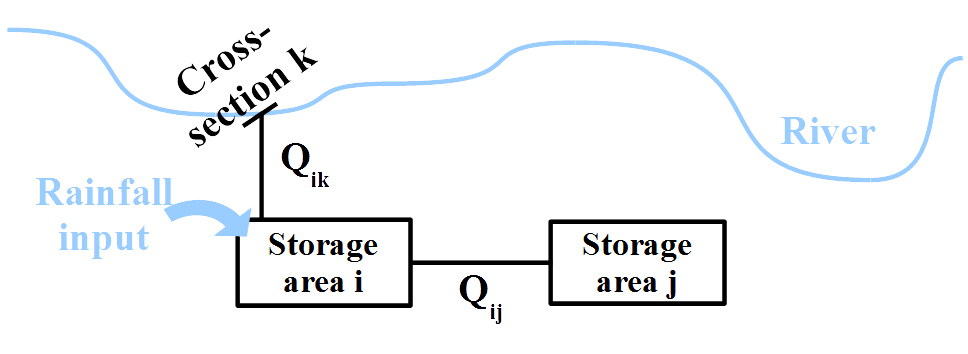
\includegraphics[width=0.8\textwidth]{Figures/CasierRiv.png}
     \caption{Principle of Storage Cell -- River interaction}
    \end{center}
\end{figure}

The flow in the river is determined by solving the one dimensional Saint-Venant equations. In the \mascaret{} system, three computational engines can be used to solve the equations: a steady transcritical engine, an unsteady subcritical engine and an unsteady transcritical engine. This chapter only covers the coupling between the storage cell system and the unsteady subcritical engine. The algorithm used in the unsteady subcritical engine is a finite difference method with an implicit scheme, the details of which are given in section \ref{CplNyFlv}.

Regarding the storage cell system, the following assumptions are made :
\begin{itemize}
 \item the free surface elevation in each storage cell is \underline{horizontal};
 \item the flow speed in the storage cells is \underline{null};
 \item the discharge in the exchange links only depends on the free surface elevation in the storage cells and/or that in the river.
\end{itemize}

Each storage cell is therefore modelled by a continuity equation, which can be written at each time step $t$ :

\begin{equation}
 \label{EqCas}
 \frac{dV_{i}(Z_i)}{dt} = \sum_j Q_{ij} (Z_i,Z_j) + \sum_k Q_{ik} (Z_i,Z_k) + Q_{input,i}
\end{equation}

where :

\begin{itemize}
 \item $i$ and $j$ are indices for the storage cells;
 \item $k$ is the index for a computation section in a reach;
 \item $V_i$ is the volume of storage cell $i$;
 \item $Z_i$ is the free surface elevation in storage cell $i$, unknown;
 \item $Z_j$ is the free surface elevation in storage cell $j$, known at the previous time step;
 \item $Z_k$ is the river level elevation in the computation section $k$, as computed by the subcritical engine;
 \item $Q_{ij}$ is the discharge flowing from storage cell $j$ towards storage cell $i$, unknown;
 \item $Q_{ik}$ is the discharge flowing from the computation section $k$ in the river towards storage cell $i$, unknown;
 \item $Q_{input,i}$ is the discharge resulting from potential contributions (rain for example) in storage cell $i$, given by the user.
\end{itemize}

The water elevation in storage cell $i$ is therefore function of the exchange flows and potential input flows.

The exchange flows $Q_{ij}$ and $Q_{ik}$ are derived by solving the equations defining the exchange links (see section \ref{DebEch}).

The elevation $Z_k$ in the river is computed by the subcritical engine. The coupling between the storage cell system and the subcritical engine is described in section \ref{CplNyFlv}. The elevation in storage cell $i$ is then computed by solving the storage cell continuity equation, detailed in section \ref{ResContCas}.

%-------------------------------------------------------------------------------
\section{Derivation of the exchange flows}
\label{DebEch}
%-------------------------------------------------------------------------------

The exchange flow through the river - storage cell links, $Q_{ik}$, or storage cell - storage cell links, $Q_{ij}$, depends on the type of connection. The solver accepts four connection types : weir link, channel link, siphon link and orifice link.

%...............................................................................
\subsection{Weir link}
%...............................................................................

The discharge is computed from the weir formulation :

\begin{equation}
 Q = C m l \sqrt{2 g} h^{\frac{3}{2}}
\end{equation}

with :
\begin{itemize}
 \item $Q$ discharge in the link;
 \item $C$ correction coefficient (allows distinction between drowned or free flow);
 \item $m$ discharge coefficient;
 \item $l$ width of the weir;
 \item $h = Z_{u/s} - Z_{sill}$ the water depth above the weir ($Z_{u/s}$ is the elevation upstream of the weir, in the river or the storage cell, and $Z_{sill}$ is the elevation of the weir crest). The elevation upstream of the weir, $Z_{u/s}$, is provided by the flow engine.
\end{itemize}

It is therefore necessary to know the width of the weir, its elevation (representative average height) and its discharge coefficient.

It is good practice to calibrate only the discharge coefficient, the other parameters matching their associated real physical values.

\begin{CommentBlock}{Note :}
The correction coefficient, $C$, makes it possible to represent the physics of the flow by taking account of the drowned or free flow conditions on the weir. It also allows to stabilise the numerical computation when the difference in elevation between the storage cells tends towards $0$. This is why it is called correction coefficient.
\end{CommentBlock}


%...............................................................................
\subsection{Channel link}
%...............................................................................

The discharge is computed with the Manning-Strickler formulation, commonly used for free surface flows, with a check of the water depth upstream of the connection.

Two distinct cases are considered :

\begin{itemize}
 \item \textbf{Case 1} : case where the average bottom elevation of the channel is higher than the bottom elevation in the storage cells or the river (horizontal channel for example);
   \begin{figure}[H]
    \begin{center}
     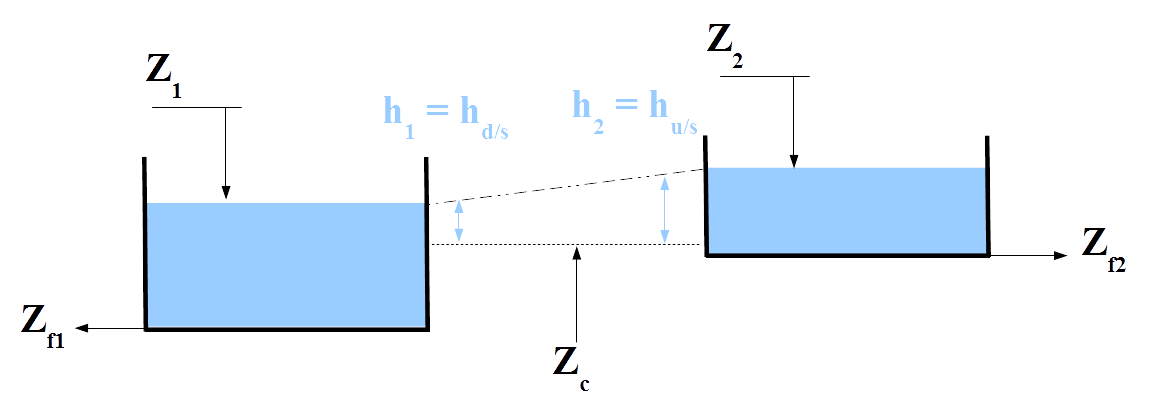
\includegraphics[width=0.8\textwidth]{Figures/Lchenal1.png}
    \end{center}
   \end{figure}
   \vspace{0.5cm}
 \item \textbf{Case 2} : case where the average bottom elevation of the channel is lower than the bottom elevation in one of the storage cells (channel with uniform slope for example).
   \begin{figure}[H]
    \begin{center}
     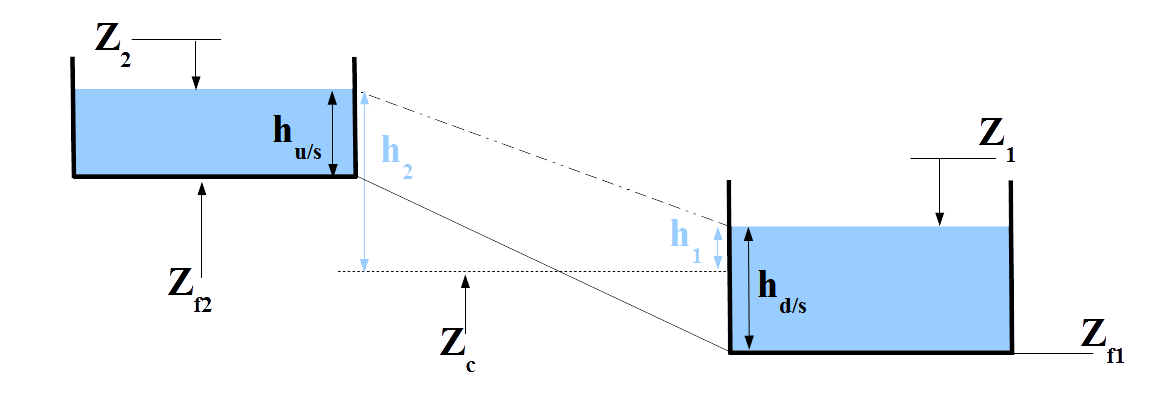
\includegraphics[width=0.8\textwidth]{Figures/Lchenal2.png}
    \end{center}
   \end{figure}
\end{itemize}

where :
\begin{itemize}
 \item $Z_1$ and $Z_2$ are the free surface elevations in the storage cells or the river;
 \item $Z_{b1}$ and $Z_{b2}$ are the bottom elevations of the storage cells or the river;
 \item $Z_c$ is the average bottom elevation of the channel;
 \item $h_1$ and $h_2$ correspond to the water depths reduced to the average bottom elevation of the channel ($h_1 = Z_1 - Z_c$ and $h_2 = Z_2 - Z_c$). They allow to determine the direction of the flow and to distinguish upstream from downstream (index 2 refers to upstream);
 \item $h_{u/s}$ and $h_{d/s}$ correspond to the real water depths upstream and downstream of the connection. In case 1, they are computed relative to the average bottom elevation of the channel and are therefore equal to $h_1$ and $h_2$ respectively. In case 2, they are computed relative to the bottom elevations of the storage cells or the river ($h_{u/s} = Z_2 - Z_{b2}$ and $h_{d/s} = Z_1 - Z_{b1}$). It is necessary to calculate these values to test the presence of water upstream of the connection. If $h_{u/s} = 0$ (whereas $h_2 > 0$), the exchange flow will be null.
\end{itemize}

The exchange flow is function of $\Delta Z = |h_1 - h_2|$ and is calculated with the Manning-Strickler formula, commomn for free surface flows :

\begin{equation}
 Q = K S R_{h}^{\frac{2}{3}} \sqrt{\frac{\Delta Z}{L}}
\end{equation}
with :
\begin{itemize}
 \item $Q$ discharge in the link;
 \item $S$ wetted cross-section of the link;
 \item $R_h$ hydraulic radius of the link;
 \item $L$ length of the link;
 \item $K$ Strickler coefficient for the link ($m^{1/3}.s^{-1}$);
 \item $\Delta Z$ difference in elevation between the two storage cells or between the storage cell and the river.
\end{itemize}

The water depth in the channel $h$ is the average of $h_{u/s}$ and $h_{d/s}$. It is assumed that the water depth, $h$, is much smaller than the width, $l$, of the connection and that the hydraulic radius $R_h$ can be approximated by the water depth, in other words : $h \ll l$ and $R_h \simeq h$.

With these assumptions, the previous equation becomes :

\begin{equation}
 Q = K l h^{\frac{5}{3}} \sqrt{\frac{\Delta Z}{L}}
\end{equation}

However, when the elevation difference $\Delta Z$ tends towards $0$, this formulation is difficult to deal with, because the derivative of the flow relative to the difference in elevation then tends towards infinity. Numerically, this problem is addressed by introducing a correction coefficient $C$. This coefficient is automatically computed by the solver. The discharge then becomes :

\begin{equation}
 Q = C K l h^{\frac{5}{3}} \sqrt{\frac{\Delta Z}{L}}
\end{equation}

Therefore, to model this type of connection, it is necessary to know the average bottom elevation of the channel, its width, its length as well as its roughness coefficient. These parameters are supplied via the *.cas file or via the user interface.

It is good practice to try and calibrate only the roughness coefficient, the other parameters matching their associated real physical values.

%...............................................................................
\subsection{Siphon link}
%...............................................................................

The discharge is computed with the general equation for pressurised flows :

\begin{equation}
 Q = \sqrt{\frac{2 g}{\lambda L}\Delta Z} \times S^{\frac{5}{4}}
\end{equation}
with :
\begin{itemize}
 \item $Q$ discharge in the link;
 \item $S$ section of the siphon;
 \item $L$ length of the siphon;
 \item $\Delta Z$ the difference in elevation between the two storage cells or between the storage cell and the river, computed by the solver;
 \item $\lambda$ head loss coefficient with respect to the walls of the tunnel (from the Moody chart).
\end{itemize}

The siphon is considered pressurised when one of its extremities is covered with water. If the siphon is not pressurised (free surface flow), the siphon link is treated like a channel link, with the width calculated as the square root of the section $S$, and the Strickler coefficient calculated as :

\begin{equation}
 K = \sqrt{\frac{2 g}{\lambda} S^{\frac{1}{6}}}
\end{equation}

When the elevation difference $\Delta Z$ tends towards $0$, the discharge formulation above becomes unstable \cite{RISSOAN02}. As for the channel link, it is necessary to introduce a correction coefficient $C$. The flow formulation can then be rewritten :

\begin{equation}
 Q = C \sqrt{\frac{2 g}{\lambda L}\Delta Z} \times S^{\frac{5}{4}}
\end{equation}

Therefore, to model this type of connection, it is necessary to know the average bottom elevation of the siphon, its length and its section as well as the head loss coefficient, $\lambda$. These parameters are supplied via the *.cas file or via the user interface.

It is good practice to calibrate only the $\lambda$ coefficient, the other parameters matching their associated real physical values.

%...............................................................................
\subsection{Orifice link}
%...............................................................................

The figure below presents the methodology diagram for this type of connection :

\begin{figure}[H]
 \begin{center}
  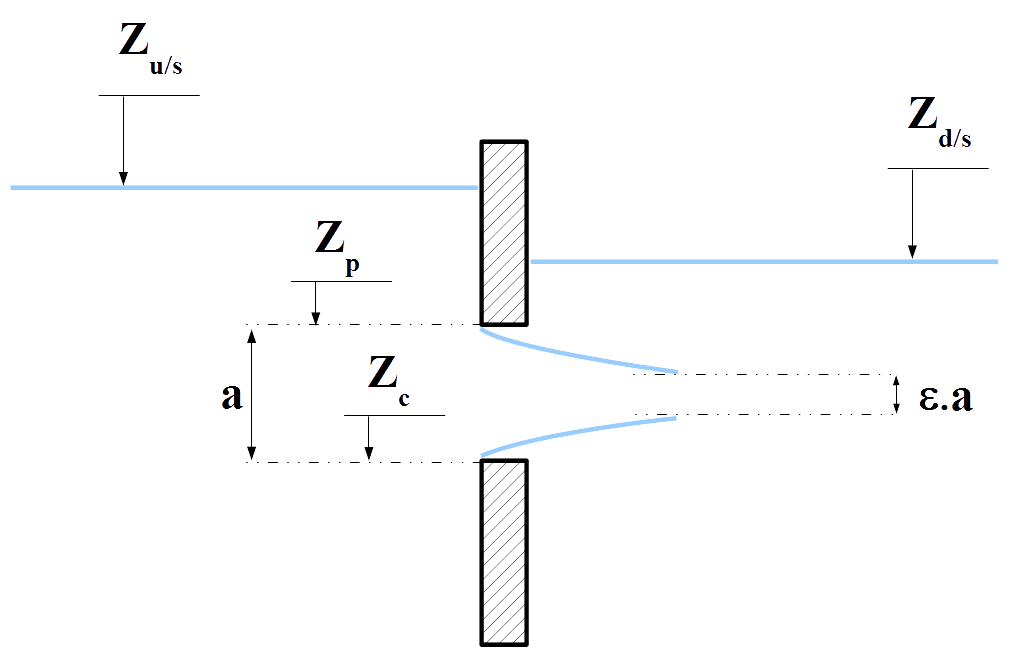
\includegraphics[width=0.8\textwidth]{Figures/Lorifice.png}
 \end{center}
\end{figure}

where :
\begin{itemize}
 \item $Z_c$ is the invert level;
 \item $Z_p$ is the soffit level;
 \item $a=Z_p - Z_c$ is the height of the opening;
 \item $Z_{u/s}$ is the water elevation upstream of the connection, and $h_{u/s}$ the associated water depth : $h_{u/s} = Z_{u/s}-Z_c$;
 \item $Z_{d/s}$ is the water elevation downstream of the connection, and $h_{d/s}$ the associated water depth : $h_{d/s} = Z_{d/s}-Z_c$;
 \item $\epsilon$ is the contraction coefficient (along the vertical).
\end{itemize}

The connection is also defined by :
\begin{itemize}
 \item $B$ width of the opening;
 \item $S$ section of the opening : $S = a B$;
 \item $m$ discharge coefficient;
 \item The direction of flow:
   \begin{itemize}
     \item \underline{type 1} : the flow is possible in the 2 directions;
     \item \underline{type 2} : the flow is only possible in the direction upstream storage cell --> downstream storage cell or storage cell --> river;
     \item \underline{type 3} : the flow is only possible in the direction downstream storage cell --> upstream storage cell or river --> storage cell.
   \end{itemize}
\end{itemize}

The values for $Z_c$, $B$, $S$ and $m$ as well as the type of valve are specified by the user in the *.cas file or via the user interface. Parameters $a$ and $Z_p$ are calculated by the solver : $a = \frac{S}{B}$ and $Z_p = Z_c + a$.

The coefficient of vertical contraction, $\epsilon$, is calculated by the solver according to the height of the opening and the load ($h_{u/s}$) :

\begin{itemize}
 \item[*] if $0 \leq \frac{a}{h_{u/s}} < 0.55$ : $\epsilon = 0.65$;
 \item[*] if $0.55 \leq \frac{a}{h_{u/s}} < 0.9$ : $\epsilon = 0.5 + 0.268 \frac{a}{h_{u/s}}$;
 \item[*] if $0.9 \leq \frac{a}{h_{u/s}} \leq 1$ : $\epsilon = 0.745 + 0.255 \left ( \frac{a}{h_{u/s}} -0.9 \right )$.
\end{itemize}

The discharge calculation then depends on the type of flow :

\begin{itemize}
 \item \textbf{free surface flow} : $Z_{u/s} < Z_p$ \\
    The orifice behaves like a weir. The discharge is calculated as for the weir link, the modular limit $\alpha$ is set to 0.2 (see section \ref{CoefAct}). The elevation of the weir crest is taken equal to $Z_c$, its width to $B$. The discharge coefficient is taken from the *.cas file. The user must therefore specify two values for the discharge coefficient: one for a weir formulation and one for an orifice formulation;
 \item \textbf{drowned surcharged flow} : $Z_{u/s} > Z_p$ et $h_{d/s} > \frac{a}{2}$ \\
    The discharge is calculated using the following formulation :
    \begin{equation}
      Q = m \epsilon S \sqrt{2 g (h_{u/s}-h_{d/s})}
    \end{equation}
 \item \textbf{free surcharged flow} : $Z_{u/s} > Z_p$ et $h_{d/s} < \frac{a}{2}$ \\
    The discharge is computed using the following formulation :
    \begin{equation}
      Q = m \epsilon S \sqrt{2 g (h_{u/s}-\frac{a}{2})}
    \end{equation}
\end{itemize}

Finally, the calculation of the exchange flow velocity depends whether the orifice is surcharged or not :

\begin{itemize}
 \item \textbf{if the orifice is surcharged} :
   \begin{equation}
     V_{exch} = \frac{Q_{exch}}{S}
   \end{equation}
 \item \textbf{if the orifice is not surcharged} :
   \begin{equation}
     V_{exch} = \frac{Q_{exch}}{S_m}
   \end{equation}
   where $S_m = B . (Z_{avg}-Z_c)$ is the average wet surface above the connection. The average water level, $Z_{avg}$, is computed by the following formulations:
   \begin{itemize}
     \item if $Z_{d/s} < Z_c$ then $Z_{avg} = \frac{Z_{u/s}+Z_c}{2}$;
     \item if $Z_{d/s} > Z_c$ then $Z_{avg} = \frac{Z_{u/s}+Z_{d/s}}{2}$.
   \end{itemize}
\end{itemize}



%...............................................................................
\subsection{Drowning coefficient or correction coefficient}
\label{CoefAct}
%...............................................................................

%...............................................................................
\subsubsection{Need for a correction coefficient}
%...............................................................................

In the case of a weir link, when the flow becomes drowned, it is necessary to use the downstream elevation in the calculation of the discharge. The downstream elevation is introduced through the drowning coefficient, $C$.

Validation of the solver \cite{RISSOAN02} has shown that numerical instabilities occur, irrespective of the type of connection, when the difference in elevation between the storage cells or between a storage cell and the river tends towards 0. The drowning coefficient then also serves to stabilise the computation. This is why it is also called correction coefficient.

In the case of a weir link, the drowning coefficient is also used as correction coefficient. In the case of channel and siphon links, no drowning coefficient is required and a correction coefficient alone is applied.
The definition of the correction coefficient matches that used for the weir link.

%...............................................................................
\subsubsection{Definition of the $C$ function}
%...............................................................................

In the unsteady subcritical engine, drowned weirs are treated using a drowning coefficient, $C$, which is function of the variable, $R$ :

\begin{equation}
  R = \frac{Z_{d/s}-Z_{crest}}{Z_{u/s}-Z_{crest}}
\end{equation}

where $Z_{crest}$ is the elevation of the weir crest. Function $C$ has a parabolic shape; its derivative is not continuous around $1$. However, when solving the storage cells system, the derivative of the discharge appears explicitly in the computations \cite{GOUTAL_RISSOAN02}. It is therefore necessary that the $C$ function and its derivative are continuous.

On the other hand, the $C$ function depends on a parameter $\alpha$, which defines the activation period of the $C$ function. $C$ is thus defined only for : $R > \alpha$. In the case of a drowned weir link, the $\alpha$ coefficient corresponds to the drowned flow criteria.

The polynomial function $C(R,\alpha)$ has to satisfy the following conditions :

\begin{eqnarray}
  C(R=\alpha)=1 & \mbox{and} & C(R=1)=0 \nonumber \\
  \frac{dC}{dR}(R=\alpha)=0 & \mbox{and} & \frac{dC}{dR}(R=1)=0 \nonumber \\
  \frac{d^2 C}{dR^2}(R=\frac{1+\alpha}{2})=0
\end{eqnarray}

This results in a third order function instead of the parabolic function used in the subcritical engine for weirs in rivers. In addition to the continuity of its derivatives, this formulation yields a faster reduction of the discharge when the levels of the two connected storage cells become closer.

The selected function is defined as follows :
\begin{itemize}
 \item in free flow mode and without correction : $R<\alpha$ and $C=1$;
 \item in drowned mode and/or with correction : $R>=\alpha$ ($R<1$ in all the cases) and :
   \begin{equation}
     C = -2 \left ( \frac{1-R}{1-\alpha} \right )^3 + 3 \left ( \frac{1-R}{1-\alpha} \right )^2
   \end{equation}
\end{itemize}

The $\alpha$ parameter is set to 0.95 for the channel and siphon links and varies between 0.2 and 0.8 for the weir links. It is set by the user according to the type of weir.

The variable $R$ is calculated relative to the $Z_{crest}$ elevation, which corresponds to the elevation of the weir crest, or to the average bottom level of the channel or that of the siphon.

\begin{figure}[H]
  \begin{center}
    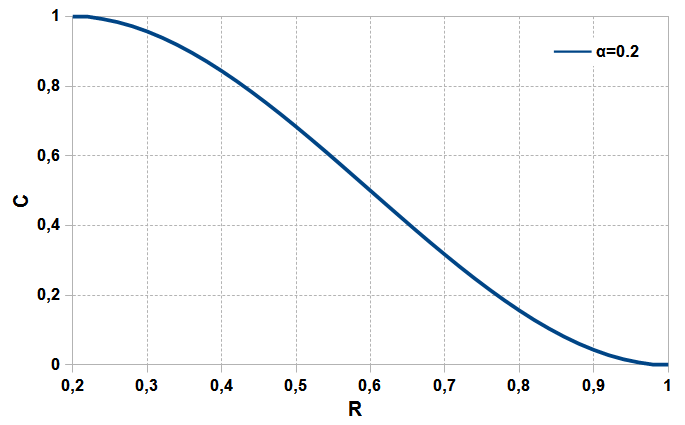
\includegraphics[width=\textwidth]{Figures/CR.png}
    \caption{Function $C=f(R)$}
  \end{center}
\end{figure}

%...............................................................................
\subsection{Contribution of rain}
%...............................................................................

The user specifies the flows due to rainfall through the definition of a hydrograph $Q(t)$. The discharge at time $t$ is taken as an average of the provided discharges at times $t$ and $t - dt$. The interpolation of the flows from the hydrograph is linear.

%-------------------------------------------------------------------------------
\section{Coupling with the subcritical engine}
\label{CplNyFlv}
%-------------------------------------------------------------------------------

The storage cells and the river are implicitly coupled with the help of a state-transition matrix \ref{eq1}. Two new equations are introduced to reflect :

\begin{itemize}
 \item the exchange flow in the links;
   \begin{equation}
     A_{link}\Delta Q_{link}+B_{link}\Delta Z_{u/s} + C_{link}\Delta Z_{d/s} = D_{link}
   \end{equation}
 \item and the change of the water level in the storage cells;
    \begin{equation}
     S_{cell}\frac{\Delta Z_{cell}}{\Delta t} = \Sigma Q_{link}
   \end{equation}
\end{itemize}

where $S_{cell}$ is the surface of a storage cell and :

\begin{equation*}
 A_{link} = -1 \mbox{ ; } B_{link} = \frac{\partial Q}{\partial Z_{u/s}} \mbox{ ; }  C_{link} = \frac{\partial Q}{\partial Z_{d/s}} \mbox{ ; } D_{link} = 0
\end{equation*}

For each storage cell anf each connection, the size of system \ref{eq1} is increased with one variable and one equation. In the case of a river - storage cell link, the shallow water equations on the corresponding river cross-sections are replaced.
The continuity equation becomes an equality between the flow discharges and the momentum equation is an equality between the water levels.

For the simple case of a reach with only 7 cross-sections, the initial shallow water system of equations is :

\begin{equation}
    \left(
         \begin{array}{cccccccccccc}
          \scriptscriptstyle -J & \scriptscriptstyle G & \scriptscriptstyle H & & & & & & & & & \\
           \scriptscriptstyle -O & \scriptscriptstyle L & \scriptscriptstyle M & & & & & & & & & \\
              & \scriptscriptstyle -I & \scriptscriptstyle -J & \scriptscriptstyle G & \scriptscriptstyle H & & & & & & & \\
              & \scriptscriptstyle -N & \scriptscriptstyle -O & \scriptscriptstyle L & \scriptscriptstyle M & & & &  & & & \\
              & & & \scriptscriptstyle -I & \scriptscriptstyle -J & \scriptscriptstyle G & \scriptscriptstyle H & & & & & \\
              & & & \scriptscriptstyle -N & \scriptscriptstyle -O & \scriptscriptstyle L & \scriptscriptstyle M & & & & & \\
              & & & & & \scriptscriptstyle -I & \scriptscriptstyle -J & \scriptscriptstyle G & \scriptscriptstyle H & & & \\
              & & & & & \scriptscriptstyle -N & \scriptscriptstyle -O & \scriptscriptstyle L & \scriptscriptstyle M & & & \\
              & & & & & & & \scriptscriptstyle -I & \scriptscriptstyle -J & \scriptscriptstyle G & \scriptscriptstyle H & \\
              & & & & & & & \scriptscriptstyle -N & \scriptscriptstyle -O & \scriptscriptstyle L & \scriptscriptstyle M & \\
              & & & & & & & & & \scriptscriptstyle -I & \scriptscriptstyle -J & \scriptscriptstyle G \\
              & & & & & & & & & \scriptscriptstyle -N & \scriptscriptstyle -O & \scriptscriptstyle L \\
         \end{array}
    \right)
    \left(
            \begin{array}{c}
               \scriptscriptstyle \Delta Z_1\\
               \scriptscriptstyle \Delta Q_2\\
               \scriptscriptstyle \Delta Z_2\\
               \scriptscriptstyle \Delta Q_3\\
               \scriptscriptstyle \Delta Z_3\\
               \scriptscriptstyle \Delta Q_4\\
               \scriptscriptstyle \Delta Z_4\\
               \scriptscriptstyle \Delta Q_5\\
               \scriptscriptstyle \Delta Z_5\\
               \scriptscriptstyle \Delta Q_6\\
               \scriptscriptstyle \Delta Z_6\\
               \scriptscriptstyle \Delta Q_7
            \end{array}
    \right)
     =
    \left(
            \begin{array}{c}
               \scriptscriptstyle K\\
               \scriptscriptstyle P\\
               \scriptscriptstyle K\\
               \scriptscriptstyle P\\
               \scriptscriptstyle K\\
               \scriptscriptstyle P\\
               \scriptscriptstyle K\\
               \scriptscriptstyle P\\
               \scriptscriptstyle K\\
               \scriptscriptstyle P\\
               \scriptscriptstyle K\\
               \scriptscriptstyle P
            \end{array}
    \right)
\end{equation}

A storage cell with a link in between the river cross-sections $4$ and $5$ gives the following system :

\begin{equation}
    \left(
         \begin{array}{cccccccccccccc}
          \scriptscriptstyle -J & \scriptscriptstyle G & \scriptscriptstyle H & & & & & & & & & & &\\
           \scriptscriptstyle -O & \scriptscriptstyle L & \scriptscriptstyle M & & & & & & & & &  & &\\
              & \scriptscriptstyle -I & \scriptscriptstyle -J & \scriptscriptstyle G & \scriptscriptstyle H & & & & & & &  & &\\
              & \scriptscriptstyle -N & \scriptscriptstyle -O & \scriptscriptstyle L & \scriptscriptstyle M & & & &  & & &  & &\\
              & & & \scriptscriptstyle -I & \scriptscriptstyle -J & \scriptscriptstyle G & \scriptscriptstyle H & & & & &  & &\\
              & & & \scriptscriptstyle -N & \scriptscriptstyle -O & \scriptscriptstyle L & \scriptscriptstyle M & & & & &  & &\\
              & & & & & \scriptscriptstyle 1 & & \scriptscriptstyle -1 & & & &  & &\\
              & & & & & & \scriptscriptstyle 1 & & \scriptscriptstyle -1 & & &  & &\\
              & & & & & & & \scriptscriptstyle -I & \scriptscriptstyle -J & \scriptscriptstyle G & \scriptscriptstyle H &  & &\\
              & & & & & & & \scriptscriptstyle -N & \scriptscriptstyle -O & \scriptscriptstyle L & \scriptscriptstyle M &  & &\\
              & & & & & & & & & \scriptscriptstyle -I & \scriptscriptstyle -J & \scriptscriptstyle G  & &\\
              & & & & & & & & & \scriptscriptstyle -N & \scriptscriptstyle -O & \scriptscriptstyle L  & &\\
              & & & & & & \scriptscriptstyle B & & \scriptscriptstyle C & & & & \scriptscriptstyle A &\\
              & & & & & & & & & & & &  \scriptscriptstyle -1 & \scriptscriptstyle \frac{S}{\Delta t}\\
         \end{array}
    \right)
    \left(
            \begin{array}{c}
               \scriptscriptstyle \Delta Z_1\\
               \scriptscriptstyle \Delta Q_2\\
               \scriptscriptstyle \Delta Z_2\\
               \scriptscriptstyle \Delta Q_3\\
               \scriptscriptstyle \Delta Z_3\\
               \scriptscriptstyle \Delta Q_4\\
               \scriptscriptstyle \Delta Z_4\\
               \scriptscriptstyle \Delta Q_5\\
               \scriptscriptstyle \Delta Z_5\\
               \scriptscriptstyle \Delta Q_6\\
               \scriptscriptstyle \Delta Z_6\\
               \scriptscriptstyle \Delta Q_7 \\
               \scriptscriptstyle \Delta Q_l \\
               \scriptscriptstyle \Delta Z_c
            \end{array}
    \right)
     =
    \left(
            \begin{array}{c}
               \scriptscriptstyle K\\
               \scriptscriptstyle P\\
               \scriptscriptstyle K\\
               \scriptscriptstyle P\\
               \scriptscriptstyle K\\
               \scriptscriptstyle P\\
               \scriptscriptstyle \Sigma Q\\
               \scriptscriptstyle \Sigma Z\\
               \scriptscriptstyle K\\
               \scriptscriptstyle P\\
               \scriptscriptstyle K\\
               \scriptscriptstyle P \\
               \scriptscriptstyle D \\
               \scriptscriptstyle Q_l
            \end{array}
    \right)
\end{equation}

%-------------------------------------------------------------------------------
\section{Data pre-processing}
%-------------------------------------------------------------------------------

The engine for the storage cell system requires that the area at the free surface $S(Z)$ and the associated volume $V(Z)$ are known for each free surface elevation $Z$ in a storage cell. It is therefore necessary to define the laws $S(Z)$ and $V(Z)$, which link an area and a volume to a given elevation. These laws need to be discretised, they are not continuous functions. They have a well-defined number of pairs $(S,Z)$ and $(V,Z)$ and the increment between elevations is constant (vertical discretisation).
%The increment between the elevations is called vertical discretisation step.

The user can enter these discretised laws $S(Z)$ and $V(Z)$ \textit{manually}, i.e. by editing directly the file holding the storage cell geometry. However, these laws are often difficult to determine. Here the user can ask that they are computed automatically by the solver, after having defined the border points and the interior points characteristic of the storage cell.

The principle of automatic vertical discretisation is as follows.

$\Longrightarrow$ \textbf{Computation of the elevations}

The elevations of the interior points are sorted in ascending order in an array called $Z_{INT}$.

By definition $Z_{INT}$ is such that :

$Z_{INT}(i-1) <= Z_{INT}(i)$ for $i=2..$ number of interior points.

$Z$ is the array containing the discretised elevations.

The first discretised elevation is the lowest elevation from the interior points : \\
$Z(1) = Min(Z(i),\mbox{ }i=1..\mbox{number of interior points}) = Z_{INT}(1)$.

The elevations are then sorted in ascending order with : \\
$Z(i+1)-Z(i) = $ vertical discretisation step.

The number of elevations is equal to the chosen number of vertical discretisation steps $N_{planim}$.

The topmost elevation is defined as follows :
 \begin{eqnarray}
 Z(N_{planim}) & = & Z(1) \nonumber \\
                & + & (N_{planim}-1) \nonumber \\
                & \times & \mbox{vertical discretisation step} \nonumber
 \end{eqnarray}

$\Longrightarrow$ \textbf{Computation of the areas}

The border points define the maximum area of the storage cell ($S_{max}$) : this area is computed from the definition of the area of a polygon. If the user has chosen the computation option whereby the area can be defined independently of the elevation, the area of the storage cell is equal to $S_{max}$ irrespective of the elevation in the storage cell.

Otherwise, the first area is computed as follows :

$S(1) = S_{max} \times$ (number of interior points with reference elevation $Z(1)$) / (number of interior points)

If $Z_{max}$ is the highest elevation from the interior points :

\begin{eqnarray}
Z_{max} & = & Max(Z(i),\mbox{ }i = 1..\mbox{number of interior points}) \nonumber \\
        & = & Z_{INT}(\mbox{number of interior points}) \nonumber
\end{eqnarray}

As long as this elevation is not reached, $S(i)$ is computed as follows :

given $k$ such that : $Z_{int}(k-1) \leq Z(i) < Z_{INT}(k)$

\begin{equation}
  S_1 = \frac{k-1}{\mbox{size}(Z_{INT})}S_{max}
\end{equation}

where $\mbox{size}(Z_{INT})$ is the size of array $Z_{INT}$.

\begin{equation}
  S_2 = \frac{k}{\mbox{size}(Z_{INT})}S_{max}
\end{equation}

\begin{equation}
  \alpha = \frac{Z(i)-Z_{INT}(k-1)}{Z_{INT}(k)-Z_{INT}(k-1)}
\end{equation}

\begin{equation}
  S(i) = (1-\alpha) \times S_1 + \alpha \times S_2
\end{equation}

When $Z_{max}$ is reached or exceeded, the area is equal to the maximum area of the storage cell : $S(i) = S_{max}$.

$\Longrightarrow$ \textbf{Computation of the volumes}

With regard to volumes, the first volume is null : $V(1) = 0$ since it is associated to the bottom elevation of the storage cell, i.e. the storage cell is empty.
The other volumes are defined by the relationship :

$V(i) = V(i-1) + [(S(i-1) + S(i)) / 2] \times$ vertical discretisation step

\begin{table}
\centering
\caption{Summary table of the laws S(Z) and V(Z)}
\begin{tabular}{c|c|c}
  \textbf{Elevation, Z} &\textbf{Area, S} & \textbf{Volume, V} \\
  \hline
  \multirow{5}{*}{$Z(1) = Z_{INT}(1)$} & $S(1) = S_{max} \times$ & \multirow{5}{*}{$V(1)=0$} \\
                                       & \footnotesize{(number of interior} & \\
                                       & \footnotesize{points with reference} & \\
                                       & \footnotesize{elevation } $Z(1)$) / & \\
                                       & \footnotesize{(number of interior points)} & \\
  \hline
  $Z(i)=Z(i-1)+$ & $S(i)=S(i-1)+\Delta S$ & $V(i)=V(i-1)+$  \\
  \footnotesize{vertical discretisation step}   & $\Delta S = (1-\alpha)S_1 + \alpha S_2$ & $(S(i-1)+S(i))/2 \times$ \\
                                       &                                         & \footnotesize{vertical discretisation step} \\
  \hline
  $Z(i)\geq Z_{INT}$ \footnotesize{(number of} & \multirow{3}{*}{$S(i) = S_{max}$} & $V(i)=V(i-1)+$  \\
  \footnotesize{interior points)}            &                  &  $(S(i-1)+S(i))/2 \times$ \\
                                               &                  & \footnotesize{vertical discretisation step} \\
  \hline
  $Z$ \footnotesize{(number of steps} & $S$ \footnotesize{(number of steps} & $V(i)=V(i-1)+$  \\
  \footnotesize{of vertical discretisation)} $=Z(1)$ & \footnotesize{of vertical discretisation)} $=S_{max}$ & $(S(i-1)+S(i))/2 \times$ \\
  $+$ \footnotesize{(number of steps of} &                   & \footnotesize{vertical discretisation steps} \\
  \footnotesize{vertical discretisation }$-1$\footnotesize{)} $\times$ & & \\
  \footnotesize{vertical discretisation step} & & \\
  \hline
 \end{tabular}
\end{table}

\textsc{\textbf{Example}} :

In this example, figure \ref{fig:PlanimCasier}) shows an plan view of a storage cell and identifies the location of the interior points with associated elevations. The points are located by their coordinates $(X,Y)$.

\begin{figure}[H]
    \begin{center}
     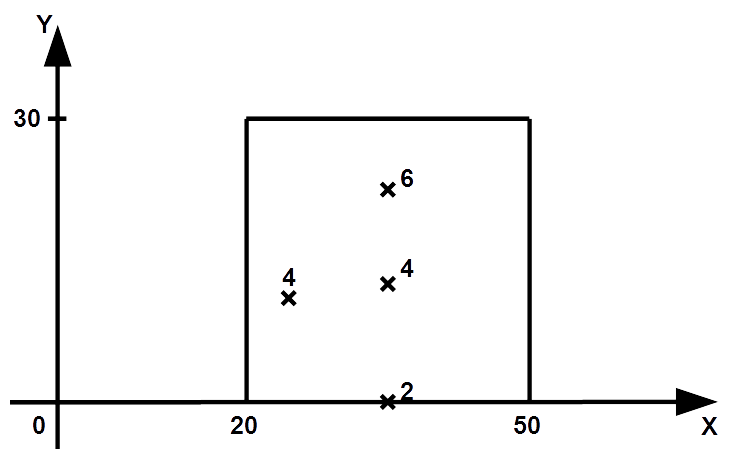
\includegraphics[width=\textwidth]{Figures/PlanimCasier.png}
     \caption{Example of vertical discretisation of a storage cell}
     \label{fig:PlanimCasier}
    \end{center}
\end{figure}

The vertical discretisation step is 1 m, the number of vertical discretisation steps is 10.

In this example, the solver determines the laws $S(Z)$ and $V(Z)$ indicated in table \ref{ExPlan}.

\begin{table}
  \centering
  \caption{Example of vertical discretisation result}
  \label{ExPlan}
  \begin{tabular}{c|c|c}
  \textbf{Elevation, Z $(m)$} &\textbf{Area, S $(m^2)$} & \textbf{Volume, V $(m^3)$} \\
 \hline
  2 & 22.5 & 0 \\
  3 & 33.8 & 28.1 \\
  4 & 67.5 & 78.8 \\
  5 & 78.8 & 151.9 \\
  6 & 90 & 236.3 \\
  7 & 90 & 326.3 \\
  8 & 90 & 416.3 \\
  9 & 90 & 506.3 \\
 10 & 90 & 596.3 \\
 11 & 90 & 686.3 \\
  \hline
  \end{tabular}
\end{table}



%----------------------------------------------------------------------------------------
%	CHAPTER 5: Automatic calibration of the Strickler coefficient
%----------------------------------------------------------------------------------------
%-------------------------------------------------------------------------------
\chapter{Automatic calibration of the Strickler coefficient}
\label{Chapter5}
%-------------------------------------------------------------------------------

\begin{WarningBlock}{Warning:}
The automatic calibration is only possible in steady state (engine \SARAP{}) and with only one reach with \mascaret{}.
\end{WarningBlock}

%-------------------------------------------------------------------------------
\section{Introduction}
%-------------------------------------------------------------------------------

For 1D and 2D hydraulic modelling based on the Saint-Venant equations, it is necessary to define a number of data including the geometry, the initial conditions in non-stationary mode, the boundary conditions and the Strickler coefficient. All these data but the Strickler coefficient are well defined by the parameters of the study (the geometry data are provided by topographical surveys; the boundary conditions and the initial conditions are defined by the study case).

The Strickler coefficient models the linear head losses attributed to friction on the bottom and the river banks. With one-dimensional modelling, however, it also accounts for dissipation phenomena which are not directly modelled. The determination of this coefficient therefore requires some calibration. This is carried out from water levels measured for flows of the same order of magnitude as those of the study.

This calibration step, which is critical for the quality of the study, is one of the most time consuming tasks in a study.

This section presents the method integrated in the \mascaret{} system and based on the solution of an adjoint problem, by which the Strickler coefficients are identified. This method shortens one of the longest tasks in applied studies and allows better control of the uncertainties related to the Strickler coefficients.

The first part presents in general terms the problem of parameters identification. The complete algorithm is then presented, applied to the case of the Strickler coefficient.

The validation of the method on several simplified cases and a real case is detailed in \cite{GOUTAL05}.

%-------------------------------------------------------------------------------
\section{Definition of the problem}
\label{PosPb}
%-------------------------------------------------------------------------------

The problem of the estimation of the Strickler coefficient is briefly presented in this section. Parameter estimation is equivalent to finding the Strickler coefficients that minimise a cost function $J$ equal to the standard deviation between the measured values and those predicted by a numerical simulation. The general principle of the existing methods to minimise a problem with several variables is reminded below.

Let us consider a steady flow in a stretch of river. A number of measurement are available that link flows to associated elevations. The purpose is to estimate, from these measurements, the Strickler coefficient (or Strickler coefficients in different areas of the model domain) which will minimise the following function $J$ :

\begin{equation}
 J(K) = \sum_{i=1..m} \alpha_i ( Z_{i}^m - Z_{i}^c (K) )^2
\end{equation}

where :
\begin{itemize}
 \item $m$ is the number of measurement points;
 \item $\alpha_i$ is a weighting factor for each measurement (this coefficient can be equal to zero if no measurement is available);
 \item $Z_{i}^m$ is the elevation measured at point $i$ for the flow considered;
 \item $Z_{i}^c$ is the elevation computed at point $i$ when solving the Saint-Venant equations with a set of Strickler coefficients $K_i$.
\end{itemize}

\begin{CommentBlock}{Note :}
\begin{itemize}
 \item $J$ is a cost function quantifying the variance between the elevation measured and that computed for a given set of Strickler coefficients;
 \item $J$ is not known analytically. To determine J, it is necessary to evaluate the elevations computed for a given set of Strickler coefficients using the Saint-Venant equations.
\end{itemize}
\end{CommentBlock}

Many methods of optimisation are presented in the literature to minimise the $J$ function. Currently, the method implemented in \mascaret{} is that used in the old version of the \texttt{CASTOR} solver \cite{LEBOSSE89_1}\cite{LEBOSSE89_2}\cite{LEBOSSE89_3}. It is a method of gradient descent.

The algorithm of gradient descent has the following general form :
\begin{itemize}
 \item[1]) estimation of the starting point;
 \item[2]) for : $k= 0,1,2...$ until convergence is reached :
   \begin{itemize}
     \item test of convergence of $x_k$;
     \item computation of the new direction of descent $d_k$;
     \item computation of the descent step $\lambda_k$: problem of non-linear minimisation with only one variable;
     \item update in the direction of descent : $x_{k+1} = x_k + \lambda_k d_k$.
   \end{itemize}
\end{itemize}

The various algorithms differ by the choice of the direction of descent and by the method used to compute the optimum step.

In the case of the method of gradient descent, the direction of descent is opposite to the gradient of the function. The complexity is in the estimation of the gradient of this function when the function itself is not known analytically. Minimisation is carried out by dichotomy and parabolic approximation when only one variable is used to find the parameter. This method of minimisation does not ensure that the minimum found is a global minimum (as opposed to a local minimum). Besides, convergence becomes very slow as the local minimum is reached.

%-------------------------------------------------------------------------------
\section{Algorithm of estimation of the Strickler coefficients}
%-------------------------------------------------------------------------------

This section presents in detail the algorithm used to estimate the Strickler coefficients in the case of a one-dimensional steady flow in a single reach. The gradient method used to minimise the cost function will also be presented.

%...............................................................................
\subsection{Reminder on the Saint-Venant equations}
%...............................................................................

The one-dimensional flow in a river is represented by a system of partial derivative equations where friction is modelled by the Strickler relation. These equations are obtained from the Navier-Stokes equations after several simplifying assumptions including :

\begin{itemize}
 \item a uniform velocity direction;
 \item a constant velocity profile in a section of the river.
\end{itemize}

In steady state, the boundary conditions are a discharge at the upstream end of the model domain and an elevation or a stage-discharge relationship at the downstream end of the domain.

The unknown factors are the elevations at every node of the computational domain : $[x_0,x_1]$. The flow is determined by the upstream boundary condition and the flow contributions along the computational domain $[x_0,x_1]$.

\begin{equation}
  \label{ContCas}
  \frac{\partial Q}{\partial x}= q_a
\end{equation}

\begin{equation}
  \label{DynCas}
  \frac{\partial}{\partial x} \left ( \frac{Q^2}{S(Z)} \right ) + g S(Z) \frac{\partial Z}{\partial x} + \frac{g Q^2}{K^2 S(Z) R^{\frac{4}{3}}} = 0
\end{equation}

\begin{equation}
 \left \lbrace
  \begin{array}{l}
    Q(x_0) = Q_{u/s} \\
    Z(x_1) = Z_{d/s}
  \end{array}
 \right.
\end{equation}

with:
\begin{itemize}
  \item $x$ the curvilinear x-coordinate along the river;
  \item $Q$ the discharge;
  \item $S(Z)$ the wetted cross-section of the river, dependent upon the elevation;
  \item $R$ the hydraulic radius, $g$ the gravity and $K$ the Strickler coefficient, as a function of $x$. In fact, this coefficient will be considered constant by zone.
\end{itemize}

The flow can be computed at all points of the computational domain from the continuity equation (\ref{ContCas}) given the flow imposed at the upstream boundary condition.

The momentum equation (\ref{DynCas}) is a differential equation which is discretised using a finite difference scheme. After discretisation, the equation to solve is of the form : $Z=F(Z)$.

This is equivalent to solving for the roots of function : $Z-F(Z)$. Each time the Saint-Venant equations are to be solved, the steady state subcritical is called. For more details, the reader is referred to the section introducing the principles of the steady state subcritical engine.

The solution to this differential equation, i.e. the elevations computed in each discrete point of the domain, depends on the Strickler coefficient. This coefficient is not known a priori but results from the calibration of the model.

%...............................................................................
\subsection{Detailed presentation of the minimisation algorithm}
%...............................................................................

In the presentation of the algorithm, the step where the discrete Saint-Venant equations are solved in steady state is called \textit{solution of the Saint-Venant equations in steady state for a discrete set of Strickler coefficients defined by zone}.

The minimisation problem presented in section \ref{PosPb} is considered. The algorithm for parameter estimation can be explained as follows :

\begin{itemize}
  \item \textbf{Step 1} : Initialisation \\
   A spatially constant Strickler coefficient is selected over the whole domain, i.e. a vector : $K_i \quad i=1..m$, $m$ being the number of zones for the Strickler coefficients;
  \item \textbf{Step 2} : Computation of the direction of descent, equal to the gradient of function $J$ with respect to vector $K$. \\
    The gradient of $J$ is not immediately known because $J$ is not known analytically.
    $J$ is a function of the various values taken by the Strickler coefficient in each zone. Each partial derivative with respect to a component will be approximated by a Taylor expansion.
    \begin{equation}
      \frac{\partial J(K(K_i))}{\partial K_i} \simeq \frac{J(K(K_i+dK_i))-J(K)}{dK_i}
    \end{equation}
    The Saint-Venant equations are solved for each component $K_i$ of the vector representing \textit{the constant Strickler coefficient by zones}, incremented by the discretisation step $dK_i$. There are as many Saint-Venant problems to solve as there are different Strickler zones.
    This gradient corresponds to the gradient of the discrete problem and not that of the continuous problem.
    \underline{Notes} : In transient state, the computation of the gradient $\frac{\partial J}{\partial S_k}$ could not be carried out by this method :
    \vspace{0.5cm}
    For $n$ time steps varying between $1$ and $M$, and $m$ measurement points, the gradient can be expressed as follows :
    \begin{equation}
      \frac{\partial J}{\partial S_k} = 2 \sum_{i,n} U_{i}^n (Z_{i}^n - m_{i}^n)
    \end{equation}
    with : $U_{i}^n = \frac{\partial Z_{i}^n}{\partial S_k}$
    \vspace{0.5cm}
    For each simulation time step and for each measurement point, the Saint-Venant equations must be solved to evaluate the gradient.
  \item \textbf{Step 3} : Minimisation in the direction of descent \\
    The problem is as follows: to minimise the function $J$ in the direction opposite that of the gradient, i.e. to find $\rho$ minimising : \\
    $J \left ( K_k - \rho \frac{\partial J(K_k)}{\partial K} \right )$ where $J$ is a non-linear function.
    The idea behind the estimation of $\rho$ is to find by dichotomy a configuration such that for 3 points $\rho_1$,$\rho_2$ and $\rho_3$ : $\rho_1<\rho_2<\rho_3$, $J(\rho_2)<J(\rho_1)$ and $J(\rho_2)<J(\rho_3)$.
    The function $J$ can then be locally approximated by a parabola. The optimal $\rho$ parameter is the minimum of this parabola, which can be computed analytically.
    The determination of the 3 points $(\rho_1,\rho_2,\rho_3)$ is done by dichotomy. For each estimate of function $J$, a Saint-Venant problem is solved.
  \item \textbf{Step 4} : Increment in the direction of descent \\
    $K_{k+1} = K_{k} - \rho \nabla J_{k}$
  \item \textbf{Step 5} : Testing convergence \\
    $\| J(K_{k+1}) \|< \epsilon$
\end{itemize}

\begin{CommentBlock}{Note :}
This method only finds local minima. Although this minimisation technique is relatively old, it has the advantage of being very simple to implement.
\end{CommentBlock}

%-------------------------------------------------------------------------------
\section{Method of calibration for compound channels}
%-------------------------------------------------------------------------------

The Strickler coefficients for the river bed (low flow channel) and floodplains (high flow channel) are defined by zones to reproduce measured water levels corresponding to bankfull and overtopping flows. As a first step, the Strickler coefficients for the river bed are estimated from the water levels measured for the bankfull flow using the automatic calibration algorithm. In a second step, the Strickler coefficients for the floodplain are then estimated using the calibrated Strickler coefficients for the river bed and the water levels measured for the overtopping flow, using again the automatic calibration algorithm.

%-------------------------------------------------------------------------------
\section{Validation and conclusions}
%-------------------------------------------------------------------------------

The algorithm for parameter estimation was initially validated on an idealised test case, such that the results obtained could be checked. The algorithm was then applied to a real study.

In steady state, automatic calibration of the Strickler coefficient is carried out using a method of parameter estimation and the computation of the cost function gradient. This approach gives satisfactory results for both idealised and real test cases. It is, however, noted that convergence is relatively slow, especially near a local minimum. In practice, the accuracy obtained with this approach is sufficient: it is indeed not realistic to expect a better accuracy than $1cm$ away from the measured levels.

Future developments will focus on the calibration for the unsteady flow state (introducing the adjoint problem to evaluate the gradient of the cost function) and on the improvement of the minimisation method (introducing more robust and more recent methods such as the conjugate gradient method or Quasi-Newton methods).



%===========================================================================
% Bibliography
%===========================================================================
\bibliographystyle{plainnat}
\bibliography{latex/mascaret_theory_guide}

\end{document}
